\documentclass[11pt,letterpaper]{article}
\usepackage[T1]{fontenc}
\usepackage[utf8]{inputenc}
\usepackage{lmodern}
\usepackage[margin=1in,headheight=15pt]{geometry}
\usepackage{amsmath,amssymb,amsthm,mathtools}
\usepackage{microtype,booktabs,longtable,array,enumitem}
\usepackage[dvipsnames]{xcolor}
\usepackage{fancyhdr,needspace}
\usepackage{listings}
\usepackage{tikz}
\usetikzlibrary{arrows.meta,positioning}
\usepackage{xurl}
\usepackage[colorlinks=true,linkcolor=MidnightBlue,citecolor=MidnightBlue,urlcolor=MidnightBlue]{hyperref}
\hypersetup{pdftitle={Groups as Diophantine Substrates},pdfauthor={AI-assisted research report prepared for Vladimir Reshetnikov},pdfsubject={Arithmetic van Kampen certificates, three commutative phases, pair order and affine matrix inputs: low-degree Diophantine certificates through the integral Heisenberg group}}
\urlstyle{same}
\pagestyle{fancy}
\fancyhf{}
\fancyhead[L]{\small Groups as Diophantine Substrates}
\fancyhead[R]{\small Research report}
\fancyfoot[C]{\thepage}
\setlength{\parskip}{0.35em}
\setlength{\parindent}{1.1em}
\setlist{itemsep=0.3em,topsep=0.4em}
\emergencystretch=2em
\allowdisplaybreaks[2]
\newtheorem{theorem}{Theorem}[section]
\newtheorem{lemma}[theorem]{Lemma}
\newtheorem{proposition}[theorem]{Proposition}
\newtheorem{corollary}[theorem]{Corollary}
\theoremstyle{definition}
\newtheorem{definition}[theorem]{Definition}
\newtheorem{example}[theorem]{Example}
\newtheorem{question}[theorem]{Question}
\theoremstyle{remark}
\newtheorem{remark}[theorem]{Remark}
\newcolumntype{L}[1]{>{\raggedright\arraybackslash}p{#1}}
% Source 03 (Part I) macros
\newcommand{\Z}{\mathbb Z}
\newcommand{\N}{\mathbb N}
\newcommand{\R}{\mathbb R}
\newcommand{\Pp}{\mathcal P}
\newcommand{\F}{F(a,b)}
\newcommand{\San}{\mathcal S}
\newcommand{\Area}{\operatorname{Area}}
\newcommand{\pc}{\operatorname{pc}}
\newcommand{\adj}{\operatorname{adj}}
\newcommand{\SL}{\operatorname{SL}}
\newcommand{\cost}{\operatorname{cost}}
\newcommand{\norm}[1]{\left\lVert #1\right\rVert}
\newcommand{\smallmat}[4]{\begin{pmatrix}#1&#2\\#3&#4\end{pmatrix}}
\newcommand{\sha}{\texttt{c58206ca101d4744a015a0f0104646109357d943}}
% Source 05 (Part II) macros
\newcommand{\ZZ}{\mathbb Z}
\newcommand{\NN}{\mathbb N}
\newcommand{\HH}{\mathsf H}
\newcommand{\calA}{\mathcal A}
\newcommand{\calB}{\mathcal B}
\newcommand{\calT}{\mathcal T}
\newcommand{\bn}{\mathfrak b}
\newcommand{\id}{\mathbf 1}
\newcommand{\supp}{\operatorname{supp}}
\newcommand{\rank}{\operatorname{rank}}
\newcommand{\diag}{\operatorname{diag}}
\newcommand{\im}{\operatorname{im}}
\newcommand{\htn}{\operatorname{ht}}
\DeclareMathOperator{\Fact}{Fact}
\DeclareMathOperator{\Sol}{Sol}
% Source 06 (Part III) macros
\newcommand{\ellg}{\ell}
\newcommand{\Spec}{\operatorname{Spec}}
\newcommand{\gap}{\mathcal G}
\newcommand{\low}{\mathcal L}
\newcommand{\up}{\mathcal U}
\newcommand{\pos}[1]{(#1)_{+}}
\newcommand{\floor}[1]{\left\lfloor #1\right\rfloor}
\newcommand{\ceil}[1]{\left\lceil #1\right\rceil}
\newcommand{\pair}[2]{K_{#1#2}}
\newcommand{\code}[1]{\nolinkurl{#1}}
% Source 07 (Part IV) macros; its \lambda_i are written \theta_i
\newcommand{\Q}{\mathbb Q}
\newcommand{\GL}{\operatorname{GL}}
\newcommand{\Span}{\operatorname{span}_{\Q}}
\newcommand{\vv}{\boldsymbol\theta}
\newcommand{\Int}{\operatorname{Int}}
\newcommand{\tr}{\operatorname{tr}}
\newcommand{\lcm}{\operatorname{lcm}}
\newcommand{\repo}{\texttt{ProveIt}}
\newcommand{\binompoly}[2]{\binom{#1}{#2}}
% Merge
\newcommand{\wtag}{\textup{[write]}}
\newcommand{\wtagb}{\textup{[write 78]}}
\lstset{basicstyle=\ttfamily\small,breaklines=true,columns=fullflexible,keepspaces=true,showstringspaces=false,frame=single,rulecolor=\color{black!20},xleftmargin=0.3em,xrightmargin=0.3em}
\setcounter{tocdepth}{2}

\begin{document}
\hypersetup{pageanchor=false}
\begin{titlepage}
\vspace*{0.1in}
\noindent{\color{MidnightBlue}\large PROVEIT RESEARCH REPORT}\par
\vspace{0.25in}
\noindent{\Huge\bfseries Groups as Diophantine\\[0.12em] Substrates}\par
\vspace{0.25in}
\noindent{\LARGE Arithmetic van Kampen certificates, three\\[0.15em] commutative phases, pair order\\[0.15em] and affine matrix inputs}\par
\vspace{0.2in}
\noindent{\large Quartic certificates through the integral Heisenberg group}\par
\vspace{0.3in}
\noindent AI-assisted research report prepared for Vladimir Reshetnikov from four manuscripts\par
\noindent(batches~76 and~78 of ProveIt's incoming reports), October 2, 2026\par
\vspace{0.2in}
\begin{abstract}\small
Part~I (source~03) treats a fixed two-generator finite presentation as a proof-producing substrate. Through Sanov's arithmetic chart of a free subgroup of $\SL_2(\Z)$, it builds explicit integer polynomials of degree at most four whose solvability is equivalent to filling a word with at most $m$ conjugates of relators, with exactly $(2s+13)m-4$ witnesses for $s$ relators, so that the compiler's minimal allocated arity recovers filling area and the Dehn function exactly. Shared proof DAGs compile without expanding relator occurrences: for $[a^{2^k},b^{2^\ell}]$ in $\langle a,b\mid[a,b]\rangle$ the area is $2^{k+\ell}$ but exactly $k+\ell$ product gates suffice and are necessary, and the quartic has $8(k+\ell)-4$ witnesses.

Part~II (source~05) compiles every finite system of integral quadratic equations into membership in an ordered product of three free abelian subgroups of a power of the discrete Heisenberg group, with an exact bijection between solutions and factorizations. With MRDP this gives three fixed subgroups whose product has computably enumerable complete membership, proposed as a negative answer to the three-subgroup question of K\"onig, Lohrey and Zetzsche and of Roman'kov. Two commuting phases are decidable; for integer exponents this is a special case of known two-subgroup results, which the report credits.

Part~III (source~06) proves that the pair counts of three-letter words leave no holes, and compiles exact quadratic and canonical quartic certificates of word realizability in three-generator Heisenberg submonoids. Part~IV (source~07) proves that an affine unimodular input curve meets every fixed subgroup of $\SL_d(\Z)$ in a finite or exactly periodic set, so that input degree two is sharp in every dimension, and compiles polynomial circuits into a fixed free-abelian unipotent subgroup when affine coordinates are existentially quantified.

The report is AI-assisted and unrefereed; nothing in it is formalized in Lean or Rocq, and priority is not certified for any Part.
\end{abstract}
\vfill
\noindent\small\textbf{Status.} Proofs and executable finite checks; not kernel-checked. Part~II's main theorem is a proposed resolution of a published open problem. Section~\ref{gts:sec:front} states the common setup and what is not claimed; Appendix~\ref{gts:app:provenance} gives the provenance.
\end{titlepage}
\hypersetup{pageanchor=true}

\tableofcontents
\newpage

\section{Scope, common setup and conventions}\label{gts:sec:front}

\wtag\ This section was written when the two manuscripts were merged. Part~\ref{gts:part:vk} and Part~\ref{gts:part:tp} print the two sources; text there without a \wtag\ marker is the source's own. \wtagb\ Parts~\ref{gts:part:po} and~\ref{gts:part:ai} were added on 2~October 2026 from two manuscripts of batch~78. Text written then is marked \wtagb; the sentences of this section that the new Parts made incomplete were extended in place, and Appendix~\ref{gts:app:provenance} lists them.

\subsection{The four Parts}\label{gts:sec:parts}

This report is built from four AI-assisted research manuscripts (Appendix~\ref{gts:app:provenance} gives the full provenance). Two were delivered together as batch~76 of ProveIt's incoming reports (manuscripts~03 and~05) and are printed as Parts~I and~II. They are called \emph{source~03} and \emph{source~05} after the file prefixes of their shipped programs and data. Neither cites the other; they were written from different snapshots of the repository on the same day, and they share no theorem. \wtagb\ Two more, batch-78 manuscripts~09 and~13, are printed as Parts~III and~IV. They are called \emph{source~06} and \emph{source~07}, again after their file prefixes, which continue this report's own sequence and are not batch-78 manuscript numbers. Both were written on 2~October 2026 from one later snapshot of the repository, before Parts~I and~II were written into this report; neither cites the other or an earlier source, and no two of the four share a theorem. All four are complementary work on one subject: \emph{groups as Diophantine substrates}, with low-degree arithmetic certificates; the first three work through the integral Heisenberg group, and the fourth through unipotent matrix groups that contain it.

\begin{itemize}
\item \textbf{Part~\ref{gts:part:vk} (source~03), \emph{Arithmetic van Kampen certificates}.} The substrate is a finitely presented two-generator group; a word is an instance, and a product of conjugates of relators is an accepting proof. Sanov's arithmetic chart of a free subgroup of $\SL_2(\Z)$ turns each conjugator into four integers on one quadric, and the compilers are sums of squares of quadratic residuals (degree at most four) whose allocated arity records the filling area exactly (Theorems~\ref{gts:vk:thm:itinerary}, \ref{gts:vk:thm:budget} and~\ref{gts:vk:thm:arity}). Shared proof DAGs compress the area exponentially, sharply for dyadic rectangular commutators (Theorem~\ref{gts:vk:thm:grid}). Here the Heisenberg group is an \emph{area detector}: a homomorphism from the free group whose central coordinate counts relator occurrences with sign (Section~\ref{gts:vk:sec:grid}).
\item \textbf{Part~\ref{gts:part:tp} (source~05), \emph{Three commutative phases are Diophantine-universal}.} The substrate is the ordered product $\calA\calB\calT$ of three free abelian subgroups of a power $\HH^d$ of the Heisenberg group. Every integral quadratic system is compiled into such a product with an exact bijection between solutions and factorizations (Theorem~\ref{gts:tp:thm:fibres}); with MRDP this gives three fixed subgroups with computably enumerable complete product membership (Theorem~\ref{gts:tp:thm:main}), proposed as a negative answer to the three-subgroup question of K\"onig, Lohrey and Zetzsche~\cite{KLZ} and Roman'kov~\cite{Romankov}. Here the Heisenberg group is the \emph{ambient group} of a membership problem.
\item \wtagb\ \textbf{Part~\ref{gts:part:po} (source~06), \emph{Order is not a moment}.} The substrate is a submonoid of $\HH^r$ generated by three labelled elements, so a certificate must show that proposed letter and pair counts come from one common word. For three letters, fixing the multiplicities and two of the three scattered pair counts leaves a gapless interval of the third (Theorem~\ref{gts:po:thm:interval}). This gives a six-equation quadratic certificate with $2c+4$ natural witnesses (Theorem~\ref{gts:po:thm:gapcompiler}), a four-corner formula for $c=2$ (Theorem~\ref{gts:po:thm:fourcorners}) and a canonical 24-witness quartic with exactly one witness tuple per accepted profile (Theorem~\ref{gts:po:thm:canonical}). Four letters can leave arbitrarily large holes (Theorem~\ref{gts:po:thm:fourletter}). The profile certificates lift to three generators of $\HH^r$ (Theorem~\ref{gts:po:thm:lift}), and membership is decidable when the multiplicity of one generator is supplied (Theorem~\ref{gts:po:thm:decidable}). Here the Heisenberg group \emph{records order}: its central coordinates are pair counts.
\item \wtagb\ \textbf{Part~\ref{gts:part:ai} (source~07), \emph{Affine matrix inputs}.} The substrate is membership of a matrix in a fixed subgroup of $\SL_d(\Z)$, and the question is how an ordinary integer input may be loaded. An entrywise affine unimodular curve meets every subgroup in a finite or exactly periodic set of inputs, in every dimension (Theorem~\ref{gts:ai:thm:rigidity}), with an exact free basis (Theorem~\ref{gts:ai:thm:freebasis}) and a sharp period (Theorem~\ref{gts:ai:thm:period}); with the repository's quadratic loader (Theorem~\ref{gts:ai:thm:quadratic}) this makes input degree two sharp in every dimension (Corollary~\ref{gts:ai:cor:degree}). With existentially quantified affine coordinates the obstruction disappears: a $6\times6$ multiplication gadget (Theorem~\ref{gts:ai:thm:mul}) compiles every polynomial circuit into membership in a fixed free-abelian unipotent subgroup (Theorem~\ref{gts:ai:thm:compiler}). Here the Heisenberg group appears as the cyclic test subgroup $\langle h(1,1,0)\rangle$ (Section~\ref{gts:sec:heis}).
\end{itemize}

Both sources use MRDP only as an imported classical theorem, at the last step, and both state explicitly that their constructions do not give finite-fold or single-fold Diophantine representations. \wtagb\ So does source~07 (Corollary~\ref{gts:ai:cor:abuniversality}); source~06 does not use MRDP. Both new sources state single-fold certificates only for restricted relations: source~06 over complete pair profiles, not over projected targets, and source~07 for languages already forced to be finite or periodic. Each Part keeps its own definitions, letters and numbering of statements; only the Heisenberg group itself is set up once, in Section~\ref{gts:sec:heis}.

\subsection{The integral Heisenberg group}\label{gts:sec:heis}

Both sources use the same group with the same multiplication convention (source~03 in Section~\ref{gts:vk:sec:grid}, source~05 in Sections~\ref{gts:tp:sec:intro} and~\ref{gts:tp:sec:compiler}). It is printed once here. Write
\[
 \HH=\operatorname{UT}_3(\Z)
 =\left\{h(a,b,c)=
 \begin{pmatrix}1&a&c\\0&1&b\\0&0&1\end{pmatrix}:a,b,c\in\Z\right\}.
\]
Source~03 writes the element $h(x,y,z)$ as the triple $(x,y,z)\in\Z^3$ and calls the group $H$; in this report that group is always written $\HH$, because Part~\ref{gts:part:vk} also uses the letter $H$ for a height bound (Theorem~\ref{gts:vk:thm:height}). The two coordinate conventions coincide: $(x,y,z)=h(x,y,z)$, with no reordering, sign change or normalization. Direct matrix multiplication gives
\begin{align}
 h(a,b,c)h(a',b',c')
   &=h(a+a',b+b',c+c'+ab'),\label{gts:tp:eq:Hmult}\\
 h(a,b,c)^{-1}&=h(-a,-b,ab-c),\label{gts:tp:eq:Hinv}\\
 h(a,b,c)^r&=h(ra,rb,rc+ab\bn(r))\quad(r\in\Z),
 \label{gts:tp:eq:Hpower}
\end{align}
where $\bn(r)=\binom r2=r(r-1)/2$ is the integer binomial of Part~\ref{gts:part:tp} (Section~\ref{gts:tp:sec:normal}). In source~03's notation, \eqref{gts:tp:eq:Hmult} reads $(x,y,z)(x',y',z')=(x+x',y+y',z+z'+xy')$ and \eqref{gts:tp:eq:Hinv} reads $(x,y,z)^{-1}=(-x,-y,-z+xy)$.

Associativity follows by expanding the third coordinate of a triple product \textup{(source~03)}. For nonnegative $r$, \eqref{gts:tp:eq:Hpower} follows by induction. For negative $r$, use \eqref{gts:tp:eq:Hinv} and the same formula, or verify that the proposed expression is a homomorphism of the exponent using \eqref{gts:tp:eq:binadd} \textup{(source~05)}.

\wtag\ Two consequences used by both Parts follow from \eqref{gts:tp:eq:Hmult} and \eqref{gts:tp:eq:Hinv}: with $[g,k]=gkg^{-1}k^{-1}$,
\begin{equation}\label{gts:eq:commutator}
 [h(a,b,c),h(a',b',c')]=h(0,0,ab'-a'b),
\end{equation}
so every commutator is central, and the centre of $\HH$ is $\{h(0,0,c):c\in\Z\}$. In a direct power $\HH^d$ all formulas hold coordinatewise. (The identities \eqref{gts:tp:eq:Hmult}--\eqref{gts:tp:eq:Hpower} and \eqref{gts:eq:commutator} were rechecked symbolically at the write, with $r$ from $-4$ to $4$ in the power law.)

\wtagb\ Parts~\ref{gts:part:po} and~\ref{gts:part:ai} use the same group with the same convention. Source~06 writes the matrix $h(\alpha,\beta,\gamma)$ as $H(\alpha,\beta,\gamma)$ and the group as $\mathbb H$; this report writes $h(\alpha,\beta,\gamma)$ and $\HH$ (Section~\ref{gts:sec:notation}). Source~07 works in $\SL_d(\Z)$ and does not name the group, but its pencil $T(t,s)=I+tJ+sJ^2$ with $J=E_{12}+E_{23}$ is $h(t,t,s)$ and its generator $P=I+J$ is $h(1,1,0)$; by~\eqref{gts:tp:eq:Hpower}, $P^m=h(m,m,\bn(m))$, which is its equation~\eqref{gts:ai:eq:Ppowers}. Part~\ref{gts:part:tp}'s third phase uses the same binomial device in another cyclic subgroup: $h(-r,-r,\bn(r))=h(-1,-1,0)^r$ in each coordinate of~\eqref{gts:tp:eq:T}, whereas $h(1,1,0)^{-1}=h(-1,-1,1)$, so $\langle h(1,1,0)\rangle\neq\langle h(-1,-1,0)\rangle$ (Remark~\ref{gts:ai:rem:binomial}).

The two Parts use the group differently. Part~\ref{gts:part:vk} uses only the homomorphism $a\mapsto h(1,0,0)$, $b\mapsto h(0,1,0)$ from the free group and reads off the central coordinate (equation~\eqref{gts:vk:eq:heisenberg}). Part~\ref{gts:part:tp} uses the whole group: the three phase homomorphisms \eqref{gts:tp:eq:A}--\eqref{gts:tp:eq:T}, and, for the two-phase theorem, the integral logarithmic coordinate $\lambda(h(a,b,c))=2c-ab$ of Section~\ref{gts:tp:sec:two}. \wtagb\ Part~\ref{gts:part:po} uses three labelled elements of $\HH^r$ and their words; its recording map~\eqref{gts:po:eq:recording} is Part~I's homomorphism applied to one pair of letters at a time, and its logarithmic map~\eqref{gts:po:eq:logcoords} has Part~II's coordinate $\lambda$ as its third entry. Part~\ref{gts:part:ai} uses only the cyclic subgroup $\langle h(1,1,0)\rangle$ of $\SL_3(\Z)$.

\subsection{Notions and letters}\label{gts:sec:notation}

Each Part keeps its source's letters. Many letters carry different meanings in the two Parts; Table~\ref{gts:tab:notation} lists every letter used in both, so that a statement of one Part is never read with the other Part's meaning. Inside a Part, the meaning is always the one in that Part's column. In Parts~I and~II the only renamed symbol is source~03's $H$ (the Heisenberg group), written $\HH$; no normalization was changed. \wtagb\ Table~\ref{gts:tab:letters78} does the same for Parts~III and~IV, against each other and against Parts~I and~II. Two symbols of those sources are renamed, with no change of normalization: source~06's Heisenberg element $H(\alpha,\beta,\gamma)$ and group $\mathbb H$ are written $h(\alpha,\beta,\gamma)$ and $\HH$, because $H$ is a height bound in Parts~I and~II; and source~07's interpolation coordinates $\lambda_i(t)$ and vector $\boldsymbol\lambda(t)$ are written $\theta_i(t)$ and $\vv(t)$, because $\lambda$ is Part~II's logarithmic coordinate $2c-ab$.

\begin{center}
\small
\begin{longtable}{@{}p{.09\textwidth}p{.43\textwidth}p{.40\textwidth}@{}}
\caption{Letters used in both Parts~I and~II.}\label{gts:tab:notation}\\
\toprule
Letter & Part~I (source 03) & Part~II (source 05)\\
\midrule
\endfirsthead
\toprule
Letter & Part~I (source 03) & Part~II (source 05)\\
\midrule
\endhead
$\HH$ & the integral Heisenberg group (source: $H=\Z^3$) & the integral Heisenberg group $\operatorname{UT}_3(\Z)$\\
$H$ & the height bound $H_{\Pp}(n,m)$ of \eqref{gts:vk:eq:height}, and $H$ in its search cube & a height bound $H$ on $\htn(x)$ in Section~\ref{gts:tp:sec:height}\\
$h$ & number of free conjugation nodes; an integer exponent in proofs & a Heisenberg element $h(a,b,c)$\\
$A,B$ & the shear matrices $\smallmat1201$, $\smallmat1021$ of \eqref{gts:vk:eq:shears}; in software words, \texttt{A}, \texttt{B} mean $a^{-1}$, $b^{-1}$ & the phase homomorphisms $A(x,u)$, $B(y)$ of \eqref{gts:tp:eq:A}, \eqref{gts:tp:eq:B} (and their small versions \eqref{gts:tp:eq:localA}, \eqref{gts:tp:eq:localB})\\
$T$, $\calT$ & --- & the third phase $T(r)$ \eqref{gts:tp:eq:T} and its image $\calT$; not a time bound\\
$C$ & the selected relator matrix $C_i$ \eqref{gts:vk:eq:selected}; the constant $C=n+mL$ \eqref{gts:vk:eq:height}; circuit nodes $C_0,\ldots,C_3$ and $C_t=[a^t,b]$ & the normal-form matrix $C\in\Z^{m\times N}$ \eqref{gts:tp:eq:normal}\\
$D$ & a proof DAG; a fixed conjugator $D\in\San$; the words $D_t=[a^u,b^t]$ & the linear part $D\in\Z^{m\times n}$ \eqref{gts:tp:eq:normal}\\
$E$ & the chart equation $E=x+t+4xt-yz$ \eqref{gts:vk:eq:chart} & the reverse quartic $E_t$ \eqref{gts:tp:eq:quartic}; $\mathcal E$ the set of mixed pairs\\
$L$ & the maximal relator length & the $N\times n$ matrix of linear forms\\
$N$, $M$ & witness and residual counts $N_{\mathrm{it}}$, $N_{\Pp}(m)$, $N_D$, $M_{\mathrm{it}}$, $M_{\Pp}(m)$, $M_D$ & $N=n+q$ binomial coordinates; $M$ a modulus (Section~\ref{gts:tp:sec:profinite})\\
$q$ & $q=2s+1$, the number of labels & $q=|\mathcal E|$; a formal variable in $Z_t(q)$\\
$m$ & the area budget & the number of equations\\
$n$ & the word length $|w|$ & the number of variables\\
$s$ & the number of relators & an index of binomial coordinates\\
$t$ & a chart coordinate; label words $t_j$ & the target $t\in\Z^m$\\
$r$, $u$ & relators $r_j$; conjugators $u_i$; exponents in $[a^u,b^v]$ & phase parameters $r,u\in\Z^N$\\
$p$ & the number of product nodes & generators $p_i$; $p=h(1,0,0)$ in a proof\\
$\lambda$, $\ell$ & label indices $\lambda_i$; chain lengths $\ell_+,\ell_\pm$; an exponent $\ell$ & the logarithmic coordinate $\lambda$; coefficients $\ell_{ji}$; the weight $\ell(x)$\\
$c$, $d$, $e$ & cost $c(D)$; $d=k+\ell$; selectors $e_{ij}$ & constants $c$; the dimension $d$ of $\HH^d$, coefficients $d_{ji}$; coordinate vectors $e_i$ and the rank $e$ of $\Z^e$\\
\bottomrule
\end{longtable}
\end{center}

\begin{center}
\small
\begin{longtable}{@{}L{.09\textwidth}L{.27\textwidth}L{.31\textwidth}L{.21\textwidth}@{}}
\caption{\wtagb\ Letters of Parts~III and~IV that are used differently elsewhere in the report.}\label{gts:tab:letters78}\\
\toprule
Letter & Part~III (source 06) & Part~IV (source 07) & Parts~I and~II\\
\midrule
\endfirsthead
\toprule
Letter & Part~III (source 06) & Part~IV (source 07) & Parts~I and~II\\
\midrule
\endhead
$\HH$, $h$, $H$ & $\HH^r$ the direct power; $h(\alpha,\beta,\gamma)$ an element (source: $H(\alpha,\beta,\gamma)$ in $\mathbb H$) & $H$, $H_0$ finitely presented groups in Theorem~\ref{gts:ai:thm:quadratic} & $H$ height bounds; in Part~I $h$ is also a node count\\
$\lambda$, $\mu$, $\ell$ & $\ell$ the doubled logarithmic map~\eqref{gts:po:eq:logcoords}, with Part~II's $\lambda$ as third entry; $\lambda_j^\pm$, $\mu_j^\pm$ sign-split witnesses & $\theta_i$, $\vv$ interpolation coordinates (source: $\lambda_i$, $\boldsymbol\lambda$); $\ell$ a linear functional & II: $\lambda=2c-ab$; I: label indices\\
$a,b,c$ & multiplicities $n_A,n_B,n_C$ of the letters; $c$ is also the number of separators. Part~II's $2c-ab$ reads $2\gamma-\alpha\beta$ here, never $2n_C-n_An_B$ & free letters $a,b$ and $a_i=b^{-i}ab^i$ (Theorem~\ref{gts:ai:thm:quadratic}); $a_i(t)=k!\,\theta_i(t)$ & II: coordinates of $h(a,b,c)$\\
$k,p,q$ & pair counts $K_{AB},K_{AC},K_{BC}$ & $k+1$ the nilpotency index; $p$ a prime; $q(t)$, $q_i$ polynomials & I: $q=2s+1$; II: $q=|\mathcal E|$\\
$A$, $B$, $C$, $D$ & letters of the alphabet; $A_s,B_s,C_s$ target coordinates & the curve $C+nD$; $A=VBV^{-1}$; $B$ a shear and a lattice basis; $A_N$ the evaluation group; $A_i,B_i$ affine operands; $A_j$ coefficients; $D$ also a degree & I: shears $A,B$, matrix $C$, DAG $D$; II: phases $A,B$, matrices $C,D$\\
$B(\cdot)$ & --- & $B(t)=\binom t2$, Part~II's $\bn(t)$ & II: the phase $B(y)$\\
$L,U,D$ & gap functionals~\eqref{gts:po:eq:LD}; corner values $L_i,U_i$; endpoints $\low_c,\up_c$ & the curve $L(n)$ and pencil $\mathcal L$; $U(n)=I+nN$ & I: relator length $L$; II: matrices $L$, $D$\\
$T$ & $T_{ij}$ doubled pair counts & the pencil $T(t,s)=h(t,t,s)$; the hit set $T$ & II: the third phase $T(r)=h(-r,-r,\bn(r))$\\
$E$ & --- & the shear $E(t)$; $E=D(d-1)$; matrix units $E_{ij}$ & I: chart equation; II: $E_t$\\
$K$ & scattered pair counts $K_{XY}$ & a subgroup ($K$, $K_g$, $K_S$, $K'$, $K_0$) & ---\\
$P$ & the canonical quartic $P$ & $P=I+J=h(1,1,0)$; the period $P_k(e)$ & I: $p$ product nodes\\
$N$ & profile count $N(a,b,c)$ & $N=C^{-1}D$, nilpotent & I: witness counts; II: $N=n+q$\\
$r$, $d$, $g$ & $r$ Heisenberg factors; $d$ alphabet size; $g,h,j$ or $g_1,g_2,g_3$ generators & $r=\rank\Lambda$; $d$ matrix size; $g$ multiplication gates & II: $r$ phase parameters, $d$ the dimension of $\HH^d$\\
$\Phi$, $\Delta$, $e$ & potential $\Phi_A$; determinants $\Delta_s$; a parity remainder $e$ & $\Phi:\Z^k\to A_N$; finite difference $\Delta$; quotient exponent $e$ & II: $e$ the rank of $\Z^e$\\
$S$ & gap-index sum $ac-p$ & a c.e.\ set & II: a c.e.\ set\\
\bottomrule
\end{longtable}
\end{center}

Five words need the same care.
\begin{itemize}
\item \textbf{Phase} (Part~\ref{gts:part:tp}) means one factor of an ordered product of commuting subgroups or submonoids: a \emph{commutative phase} is a family of pairwise commuting matrices that may be used in any order and number before the product moves to the next phase. It is not a complex phase, not a phase of the Fabius or Rvachev functions, and not a stage of the ``four-phase zero test'' in Part~XIII of the report \emph{canonical-diophantine-certificates}.
\item \textbf{History-free} (the subtitle of Part~\ref{gts:part:vk}) means that the certificate stores no conjugator \emph{word}: no word length, list of letters or matrix-multiplication history, only four chart integers per conjugator (Section~\ref{gts:vk:sec:chart}). The tempting reading is that of Part~XIV of \emph{canonical-diophantine-certificates}, ``history-free routing certificates'', where the certified object is an outcome (firing counts) rather than a time-ordered execution of a chip-routing network. The two senses are related, but they concern different histories.
\item \textbf{Compiler} in both Parts means an explicit map from a group-theoretic or arithmetic problem instance to polynomials or matrices. It is unrelated to the sparse-machine ``universal compiler'' with arithmetic-operation counts of the repository's Hilbert-tenth-problem research notes; neither Part claims or improves an arithmetic-operation record.
\item \textbf{Slice}: Corollary~\ref{gts:vk:cor:slice} of Part~I concerns a bounded-\emph{area} slice $\Area_{\Pp}(w)\leq m$; Corollary~\ref{gts:tp:cor:slice} of Part~II concerns a \emph{central} slice of the group $\HH^N\times\Z^m$.
\item \textbf{Exponents}: in Part~\ref{gts:part:tp}, integer exponents make the phases subgroups, and natural exponents make them submonoids; matrix entries may be negative in both cases.
\end{itemize}
\wtagb\ Parts~III and~IV add six more.
\begin{itemize}
\item \textbf{Moment} (Part~\ref{gts:part:po}'s title, ``moment fibre'') means a gap-index sum $\sum_i(c-i)x_i$, the number of later separators summed over the occurrences of a letter. It is not a probabilistic moment, and not Part~\ref{gts:part:ai}'s moment curve $(t,t^2,\ldots,t^k)$ (Lemma~\ref{gts:ai:lem:moment}).
\item \textbf{Phase} does not occur in Parts~III and~IV. One step of a proof of source~06 is called ``the second phase'' there; it is printed as ``the second stage'' (proof of Lemma~\ref{gts:po:lem:connected}).
\item \textbf{Pair count} in Part~\ref{gts:part:po} is the central coordinate of Part~I's area detector on a positive word; it is not a filling area.
\item \textbf{Single-fold}: Part~\ref{gts:part:po}'s canonical quartic has exactly one witness tuple over each complete pair profile, not over each projected target (Section~\ref{gts:po:sec:projection}); Part~\ref{gts:part:ai}'s certificates are single-fold over each accepted input of a language already forced to be finite or periodic (Theorem~\ref{gts:ai:thm:certificate}). Neither is a single-fold representation of c.e.\ sets.
\item \textbf{Ordinary input} and \textbf{loader} (Part~\ref{gts:part:ai}) are used as in the Hilbert-tenth-problem research notes: one integer $n$ enters a fixed matrix curve $L(n)$, with no further quantified coordinates; an \emph{existential} coordinate is a different interface~\eqref{gts:ai:eq:quantified-interface}.
\item \textbf{Exactly periodic} (Part~\ref{gts:part:ai}) means a union of residue classes on all of $\Z$, not eventually periodic; $\Spec_c$ (Part~\ref{gts:part:po}) is a set of pair counts, not a spectrum of a ring or an operator.
\end{itemize}

\subsection{Relation to the repository and to the literature}\label{gts:sec:relation}

Neither source cites the related material below, which was identified at placement; this subsection supplies the cross-references (pins and dates in Appendix~\ref{gts:app:provenance}). \wtagb\ The second list concerns Parts~III and~IV.

\begin{itemize}
\item \textbf{Report \emph{probabilistic-quantum-and-continuous-computation}, Part~VI}~\cite{pqc} (sources~11 and~16 there; its Theorem \texttt{pqc:dr:thm:main}). It compiles finite group presentations into rational rotation gates in $\mathrm{SO}(4,\Z[1/5])$ by Mihailova's fibre-product construction, obtains c.e.-complete membership for a fixed finitely generated subgroup, and certifies bounded \emph{words} in that matrix group by quartic synthesis certificates. Part~\ref{gts:part:vk} has the same input (finite presentations and their relators) but a different substrate and resource: words of a free group in $\SL_2(\Z)$, and relator \emph{area} and proof-DAG size. Part~\ref{gts:part:tp} has a statement of the same kind (a fixed c.e.-complete membership problem for fixed integer matrices) for a different object, a product of three abelian subgroups of a unitriangular group, by a different mechanism.
\item \textbf{The research note \path{group_commutator_universal_substrate.md}}~\cite{repo-comm} of the Hilbert-tenth-problem programme. For every c.e.\ set it computes a finitely generated subgroup of $\SL(4,\Z)$ whose membership along a fixed quadratic matrix curve is that set, by commutator relators, Higman's embedding theorem and Mihailova's construction. This is the same kind of universality statement as Theorem~\ref{gts:tp:thm:everyset}, for subgroup membership in $\SL(4,\Z)$ rather than for a product of three abelian subgroups of $\HH^d$. Neither it nor Part~VI of \cite{pqc} measures relator area or compiles proof DAGs, which is what Part~\ref{gts:part:vk} does.
\item \textbf{The research note \path{group_unipotent_input_loaders.md}}~\cite{repo-unip}. It proves by ping-pong that $U=\smallmat1401$ and $B=\smallmat1011$ form a free pair in $\SL_2(\Z)$ and uses it to load ordinary inputs into conjugates. Part~\ref{gts:part:vk} uses Sanov's different pair \eqref{gts:vk:eq:shears} and, crucially, its exact arithmetic \emph{image}, the integral points of one quadric (Theorem~\ref{gts:vk:thm:sanov}); the note gives no description of the image of its pair, and Part~\ref{gts:part:vk} warns that the congruence description must not be assumed for other shear parameters (the end of Section~\ref{gts:vk:sec:chart}).
\item \textbf{The research note \path{heisenberg_two_generator_membership.md}}~\cite{repo-heis}. It decides membership in every submonoid of $\HH^r$ generated by two elements, and in the commuting case it uses the injective coordinates $\ell(a,b,c)=(2a,2b,2c-ab)$, the same device as Part~\ref{gts:part:tp}'s $\lambda=2c-ab$ (Section~\ref{gts:tp:sec:two}). Its commuting case is the special case of Theorem~\ref{gts:tp:thm:two} with one generator in each phase and natural exponents. The note ends: three or more generators are necessary for undecidable membership in this substrate, ``this statement does not claim that three suffice''. \emph{Part~\ref{gts:part:tp} does not answer that question.} The note concerns a submonoid generated by three elements, which contains arbitrary interleaved words; Part~\ref{gts:part:tp} concerns an ordered product of three subgroups or submonoids, each commutative and generated by many elements, with no interleaving across phases. The note's primary source is a different paper of Roman'kov (arXiv:2209.14786, Skolem systems compiled into submonoids), not the paper~\cite{Romankov} cited in Part~\ref{gts:part:tp}. \wtagb\ (2~October 2026.) \emph{Part~\ref{gts:part:po} answers this open point in part.} It pays word realizability exactly for three generators: for a ternary alphabet the third pair count fills an interval (Theorem~\ref{gts:po:thm:interval}), with exact quadratic and quartic certificates (Theorems~\ref{gts:po:thm:gapcompiler} and~\ref{gts:po:thm:canonical}), and membership in a three-generator submonoid of $\HH^r$ is decidable when the number of occurrences of one generator is supplied (Theorem~\ref{gts:po:thm:decidable}). It also derives the exact conditional spectrum behind the note's ternary false family~\eqref{gts:po:eq:reporesolve}. The unrestricted three-generator question stays open; source~06 does not decide it (question~9 of Section~\ref{gts:po:sec:questions}). Source~06 cites that paper of Roman'kov as~\cite{po-romankov}.
\item \textbf{The research note \path{group_projective_label_aligned_lanes.md}}~\cite{repo-group} is source~03's own comparison (Section~\ref{gts:vk:sec:problem}); it is unchanged from source~03's pin to the write.
\item \textbf{Report \emph{canonical-diophantine-certificates}.} Its compilers go from bounded executions to canonical arithmetic zeros; Part~\ref{gts:part:vk}'s native compiler is explicitly not canonical (Proposition~\ref{gts:vk:prop:infinite-fibers}), and Part~\ref{gts:part:tp} compiles in the reverse direction, from arithmetic to a group, preserving fibres. Its remark that a four-squares conversion ``can introduce many witnesses for one natural value'' (in its research questions) is the same caveat as Part~\ref{gts:part:tp}'s four-square paragraph in Section~\ref{gts:tp:sec:universal}.
\item \textbf{Bounded search.} Corollary~\ref{gts:vk:cor:nonrecursive}, Theorem~\ref{gts:vk:thm:no-sharing-cutoff} and Proposition~\ref{gts:tp:prop:nobound} use the argument ``a computable bound would give a bounded search, hence a decision procedure'', as do Corollary \texttt{pqc:qm:cor:nobound} of \cite{pqc} and Proposition \texttt{cdc:bd:prop:nobound} of \emph{canonical-diophantine-certificates}. The statements are different (Dehn and sharing profiles, factorization exponents, mortal-word lengths, witness heights), so all are printed.
\end{itemize}

\wtagb\ Parts~III and~IV relate to the following material; sources~06 and~07 cite it only where said.
\begin{itemize}
\item \textbf{Part~I's area detector and Part~II's coordinate.} Part~\ref{gts:part:po}'s recording map~\eqref{gts:po:eq:recording} is the homomorphism~\eqref{gts:vk:eq:heisenberg}, one Heisenberg factor per pair of letters; on positive words its central coordinate is the scattered pair count, whereas Part~I uses it on arbitrary words to bound van Kampen area. Part~\ref{gts:part:po}'s map~\eqref{gts:po:eq:logcoords} is $(2a,2b,\lambda)$ with Part~II's $\lambda$, and its correction~\eqref{gts:po:eq:logcorrection} is~\eqref{gts:tp:eq:loglaw} summed over pairs: the third independent derivation of that device in the repository, after the note~\cite{repo-heis} and Section~\ref{gts:tp:sec:two}. No theorem of Parts~I and~II is re-proved in Part~\ref{gts:part:po}.
\item \textbf{Parikh matrices}~\cite{mssy}. For an ordered binary alphabet the Parikh matrix is the factor~\eqref{gts:po:eq:recording}; source~06 compares its profiles with 2-binomial equivalence and cites Parikh matrices only through~\cite{po-teh} (note in Section~\ref{gts:po:sec:literature}).
\item \textbf{The research note \path{group_affine_input_obstruction.md}}~\cite{ai-repoaffine}, which source~07 cites and generalizes: its paired-$\SL_2$ classification (empty, a singleton or one coset) is the case $k=1$ of Theorem~\ref{gts:ai:thm:rigidity}, and its $\SL_3$ example $\{1,2\}$ is re-derived as a case $k=2$. That note, the commutator note~\cite{repo-comm} and the programme's README restrict the degree-two conclusion to that interface, or say that it does not extend to general $\SL_3$ or $\SL_4$ curves; after Part~\ref{gts:part:ai} the restriction applies to the single-coset shape only, not to decidability or to the degree threshold (Corollary~\ref{gts:ai:cor:degree}). Those notes belong to another part of the repository and are not edited here.
\item \textbf{The commutator note}~\cite{repo-comm} (source~07's~\cite{ai-repoquadratic}). Theorem~\ref{gts:ai:thm:quadratic} is its construction, reconstructed and attributed by source~07; what Part~\ref{gts:part:ai} adds is the synthesis of Corollary~\ref{gts:ai:cor:degree}.
\item \textbf{The unipotent-loader note}~\cite{repo-unip}. Part~\ref{gts:part:ai}'s curve $Q(n)$~\eqref{gts:ai:eq:Q} is the note's swapped-basis curve $L_*(x)$ with $c=12$, and Step~4 of Theorem~\ref{gts:ai:thm:quadratic} re-derives its free pair; source~07 does not cite the note.
\item \textbf{The complete matrix-membership compiler}~\cite{repo-cmc}: a fully charged positive Diophantine certificate for membership of $\diag(L_r,L_r)$ in a fixed subgroup of $\SL_2(\Z)\times\SL_2(\Z)$ given by a supplied macro table. It does part of Part~\ref{gts:part:ai}'s question~10 (note there).
\item \textbf{The programme's affine mortality notes} (for example \path{group_affine_bipartite_mortality5.md}). They load one affine input matrix as a generator of a matrix semigroup and ask for a zero product, an interface with singular matrices and no subgroup test; they are consistent with Part~\ref{gts:part:ai} and do not overlap it.
\item \textbf{Part~VI of~\cite{pqc}} prints Mihailova's generators (\path{pqc:dr:prop:mihailova}, \path{pqc:rr:lem:mihailova}); Step~3 of Theorem~\ref{gts:ai:thm:quadratic} prints them again, as a marked second route.
\item \textbf{Part~II and Part~IV.} Theorem~\ref{gts:tp:thm:everyset} shows that Part~\ref{gts:part:ai}'s subgroup hypothesis is necessary, and that its rigidity fails for products of three subgroups even along a central affine line (Remark~\ref{gts:ai:rem:subgroup}); the two Parts share a binomial device in different cyclic subgroups (Remark~\ref{gts:ai:rem:binomial}).
\item \textbf{The programme's reviews of both archives}, written on the day of their arrival and before this placement: \cite{repo-rev808} for source~06 and~\cite{repo-revaffine} for source~07. They found no mathematical defect, replayed both programs, and prove two reductions printed as dated notes, a cheaper finalizer for Part~\ref{gts:part:po}'s quartic (after Theorem~\ref{gts:po:thm:canonical}) and one block fewer for each square gate of Part~\ref{gts:part:ai}'s compiler (after Theorem~\ref{gts:ai:thm:compiler}).
\end{itemize}

No result of the three neighbouring reports of this category (\emph{canonical-diophantine-certificates}, \emph{probabilistic-quantum-and-continuous-computation}, \emph{liveness-beyond-halting}) is re-proved in this report, so no proof was replaced by a pointer. \wtagb\ This remains true of Parts~III and~IV with one exception: Step~3 of Theorem~\ref{gts:ai:thm:quadratic} re-proves the finite generation of Mihailova's fibre product, which is \texttt{pqc:dr:prop:mihailova} of~\cite{pqc}; it is printed as a marked second route with that pointer.

\textbf{Literature credit for the two-phase theorem.} For \emph{integer} exponents, Theorem~\ref{gts:tp:thm:two} is a special case of known results: a product of two subgroups of a polycyclic group is closed in the profinite topology and therefore has decidable membership~\cite[Remark~6.7]{KLZ}, and Roman'kov proves that the product of two subgroups membership problem is decidable in every finitely generated nilpotent group of class two~\cite{Romankov}. The group $\HH^d\times\Z^e$ is both. Source~05 does not cite these results for its two-phase theorem; the credit and a precise statement of what source~05 adds are in Remark~\ref{gts:tp:rem:credit} after the theorem. The three-subgroup statement, Theorem~\ref{gts:tp:thm:main}, is different: both sources~\cite{KLZ,Romankov} state that case as open, and no earlier resolution was found at placement (a check of the arXiv text of~\cite{KLZ} and of the abstract of~\cite{Romankov}); its priority is not certified.

\subsection{Status and what is not claimed}\label{gts:sec:status}

The report is AI-assisted and unrefereed, and \textbf{nothing in it is formalized in Lean or Rocq}. Both sources give conventional proofs together with finite exact-integer checks that are illustrations, not proofs. Part~\ref{gts:part:tp}'s main theorem is a \emph{proposed} resolution of a published open problem, not a peer-reviewed or proof-assistant-checked theorem. Every limitation stated by either source is kept in its Part; collected here, neither Part claims
\begin{itemize}
\item historical priority for its constructions (both sources say so; Part~\ref{gts:part:vk}, Appendix~\ref{gts:vk:app:audit}; Part~\ref{gts:part:tp}, Appendix~\ref{gts:tp:app:audit} and Appendix~\ref{gts:tp:app:sources});
\item a finite-fold or single-fold Diophantine representation of c.e.\ sets, or of group word problems; the native fibres of Part~\ref{gts:part:vk} are generally infinite (Proposition~\ref{gts:vk:prop:infinite-fibers}), and Part~\ref{gts:part:tp} transfers fold bounds only conditionally;
\item a universal arithmetic-operation record, an improvement of the universal degree-four bound, an optimized ambient dimension, or a numerically instantiated universal presentation, polynomial or matrix table;
\item that its counts are minimal among all Diophantine representations: they are the literal counts of the stated compilers;
\item one fixed-arity polynomial with a varying number of variables: in Part~\ref{gts:part:vk} the budget $m$ and the circuit shape are external data, and the passage to a fixed arity is MRDP's, which preserves neither fibres nor the area ledger (Section~\ref{gts:vk:sec:fold});
\item any new Lean or Rocq verification.
\end{itemize}
\wtagb\ Parts~\ref{gts:part:po} and~\ref{gts:part:ai} have the same status: proofs and finite exact checks, AI-assisted, unrefereed, not formalized, priority not established, as each source says. Every limitation of sources~06 and~07 is kept in its Part; collected here, neither claims
\begin{itemize}
\item an improvement of the repository's universal arithmetic-operation bound (87 operations at the sources' pin), or a numerically instantiated universal monoid, Higman subgroup or matrix table; source~06 does not instantiate Roman'kov's undecidable submonoid;
\item a single-fold or finite-fold representation of c.e.\ sets: Part~III's canonical quartic is single-fold over a complete pair profile, not over a projected matrix target (Section~\ref{gts:po:sec:projection}), and Part~IV's single-fold certificates concern only languages already forced to be finite or periodic, while its compiler's added coordinates are unique only given the source witnesses, which a four-square substitution can multiply;
\item one fixed-arity polynomial for all separator counts $c$ (Part~III), or optimality of Part~IV's dimension $6g+2$ or of its multiplication gadget;
\item that Part~III decides three-generator membership without a supplied multiplicity, or that three generators give undecidable membership;
\item a uniform algorithm computing Part~IV's finite or periodic description from subgroup generators: Proposition~\ref{gts:ai:prop:uniform} shows that there is none;
\item that Part~IV's degree threshold bounds anything but the input degree in its stated interface; its degree-two half rests on the external effective Higman embedding~\cite{ai-mikaelian}, through the repository construction it reconstructs.
\end{itemize}

\subsection{Research questions}\label{gts:sec:questions}

Both agendas are printed in full: the twelve questions of Part~I (Section~\ref{gts:vk:sec:questions}) and the nine research directions of Part~II (Section~\ref{gts:tp:sec:future}). Neither Part answers a question of the other, and the placement survey of the repository found none of them answered there. Three pairs are related and should be read together: higher nilpotent invariants as lower-bound detectors for proof DAGs (Question~\ref{gts:vk:q:detectors}) and higher unitriangular groups as substrates for higher-degree compilers (Section~\ref{gts:tp:q:nilpotent}); the first formal milestones, the Sanov chart and fixed-itinerary compiler (Question~\ref{gts:vk:q:chart}) and the exact fibre theorem (Section~\ref{gts:tp:q:formal}), each independent of MRDP; and passing the repository's existing certificate compilers through the new constructions with fair metrics or intact fibres (Question~\ref{gts:vk:q:interop} and Section~\ref{gts:tp:q:counting}).

\wtagb\ Part~III adds twelve research questions (Section~\ref{gts:po:sec:questions}) and Part~IV ten (Section~\ref{gts:ai:sec:questions}). Two of Part~IV's are partly answered elsewhere in the repository: Part~II answers the negative half of question~9 (subgroups replaced by rational subsets) for products of three subgroups or of three free commutative submonoids (Remark~\ref{gts:ai:rem:subgroup}), and question~10 (a fully charged universal matrix certificate) is partly done by the research note~\cite{repo-cmc}; both are re-scoped at the questions. Part~III's question~11 (higher-step nilpotent groups) belongs with Question~\ref{gts:vk:q:detectors} and Section~\ref{gts:tp:q:nilpotent}, and its question~9 (three generators without a supplied multiplicity) is what remains open of the research note's question (Section~\ref{gts:sec:relation}). The placement survey found no other question of Parts~III and~IV answered in the repository.

\part{Arithmetic van Kampen certificates (source 03)}\label{gts:part:vk}

\noindent\wtag\ Part~I prints batch-76 manuscript~03, \emph{Arithmetic van Kampen Certificates: Quartic equations, exact filling area, and optimal proof-DAG compression}, subtitled \emph{A history-free Diophantine compiler for group-theoretic computation} (``history-free'' in the sense of Section~\ref{gts:sec:notation}), research report prepared for Vladimir Reshetnikov, October 2, 2026. Its labels carry the prefix \texttt{gts:vk:}. Its abstract and the artifact boundary of its title page follow.

\begin{quote}\small
\textbf{Abstract (source 03).} For a fixed two-generator finite group presentation with $s$ relators, we construct an explicit family of integer polynomials of degree at most four whose solvability at a boundary word is equivalent to filling that word with at most $m$ conjugates of defining relators. The compiler allocates exactly $(2s+13)m-4$ integer witnesses for $m\geq1$. Fixing the ordered relator choices reduces this to $8m-4$. A classical arithmetic description of a free subgroup of $\SL_2(\Z)$ eliminates conjugator-word histories: each conjugator is represented by four integers satisfying a single quadratic equation.

We give a small-witness bound, identify the minimum allocated arity of the area compiler with the presentation's filling area, and derive the precise obstruction to a computable complete area cutoff. We then compile shared group-proof circuits into quartics without expanding their relator occurrences. For
$[a^{2^k},b^{2^\ell}]$ in $\langle a,b\mid[a,b]\rangle$, the area is $2^{k+\ell}$, whereas the minimum number of product gates in the specified proof calculus is exactly $k+\ell$. The resulting fixed-conjugator quartic uses only $8(k+\ell)-4$ witnesses when $k+\ell\geq1$. A more general addition-chain sandwich bounds rectangular commutator proof complexity.

The report provides complete proofs of the compiler and compression statements, exact-arithmetic software, adversarial examples, and a formalization and research agenda. Classical inputs are identified explicitly. Priority for the particular synthesis is not established; no unrestricted finite-fold MRDP theorem, universal arithmetic-operation record, or new Lean verification is claimed.

\medskip
\textbf{Artifact boundary.} The mathematical development is a research draft with executable checks. It is not a kernel-checked extension of ProveIt. The repository snapshot used for comparison is\par
\sha.
\end{quote}

\section{The problem addressed and the contribution boundary}\label{gts:vk:sec:problem}

The broad assertion that an effectively simulable computational substrate has a Diophantine acceptance relation is already covered by MRDP. Repeating that assertion for another model of computation is usually less useful than preserving a resource that the model makes mathematically meaningful. Here that resource is \emph{filling area}: the number of relator applications needed to establish a word identity.

Our computational substrate is a finitely presented group. The finite presentation is the program, a word is the instance, and an expression of that word as a product of conjugates of defining relators is an accepting proof. This viewpoint includes systems with undecidable word problem through classical constructions. Its advantage for Diophantine compilation is that free-group elements admit a particularly economical arithmetic representation.

The central distinction is between three different resources:
\begin{equation}\label{gts:vk:eq:three-resources}
 \text{conjugator word length},\qquad
 \text{expanded relator area},\qquad
 \text{shared proof-circuit size}.
\end{equation}
The first compiler charges for the second resource but not the first. The second compiler charges for the third, without expanding the second. Integer magnitude and coefficient bit length remain separate costs throughout.

\subsection{What has been established here}

The following table is a contribution ledger, not a claim of historical priority. All numerical variable counts refer to the literal compilers specified in this report, before optional elimination or simplification.

\begin{center}
\begin{tabular}{L{0.24\textwidth}L{0.42\textwidth}L{0.23\textwidth}}
\toprule
Result & Content & Status\\
\midrule
Arithmetic free-group chart & Four integral coordinates and one quadratic determinant equation & Classical Sanov theorem; proof included\\
Fixed-itinerary compiler & $8m-4$ variables, $5m$ quadratic residuals & Explicit construction and proof here\\
Area-budget compiler & $(2s+13)m-4$ variables, $(2s+11)m$ residuals & Explicit construction and proof here\\
Witness height & An elementary height bound for at least one witness at every accepting budget & Uses a cited classical conjugator bound\\
Native arity profile & Exact affine recovery of filling area and Dehn function & Consequence for the defined compiler\\
Proof-DAG compiler & Linear allocation in the number of circuit nodes, not expanded leaves & Explicit construction and proof here\\
Optimal dyadic grids & Area $2^{k+\ell}$; exactly $k+\ell$ product gates & Sharp theorem in the specified calculus\\
Addition-chain bounds & A lower signed-chain bound and an upper ordinary-chain bound & Proved here as a refinement\\
\bottomrule
\end{tabular}
\end{center}

The main question resolved within this program is therefore concrete: \emph{can one give an explicit low-degree Diophantine certificate whose visible resource is group-theoretic proof area, and can shared proofs compress that resource with a sharp, provable gain?} The answer is yes, with the formulas and exact counts above. This is not presented as a resolution of a famous previously named open problem. The broader novelty and publication significance require further specialist comparison.

\subsection{Relationship to the repository}

ProveIt's documented MRDP endpoint produces a fixed finite polynomial representation for a recursively enumerable subset of the natural numbers; its public statement does not itself specify a practical compiler or a numerical degree or witness bound \cite{repo-mrdp}. The repository also contains an extensive native-stream/queue compiler program. In particular, the inspected group-projective note optimizes the storage positions of signed-shear controller lanes while preserving chronological macro execution \cite{repo-group}. That is a packed-history construction, not the relator-area compiler developed below.

The present work is a complementary semantic front end. We do not transfer the repository's formal-verification status to the new theorems, and we do not claim an improvement to its arithmetic-operation records. The exact chart, local matrix equations, and proof-circuit semantics below are proved directly. Only the final fixed-arity existence discussion invokes the MRDP interface at an abstract level.

\wtag\ This repository relationship is incomplete; Section~\ref{gts:sec:relation} supplies the missing comparisons. The collection's report on probabilistic, quantum and continuous computation (Part~VI of~\cite{pqc}) compiles finite presentations into rational rotation gates by Mihailova's construction and certifies bounded \emph{words} in that matrix group; the research programme's group-commutator note~\cite{repo-comm} obtains universal subgroup membership in $\SL(4,\Z)$, and its unipotent-loader note~\cite{repo-unip} proves a different free pair in $\SL_2(\Z)$ faithful without describing its image arithmetically. None of them measures relator area or compiles proof DAGs. Both repository files cited here are unchanged from the pin \sha\ to this report's write.

\subsection{Conventions that prevent misleading conclusions}

All existential variables in the displayed compilers range over $\Z$, not over positive integers. The budget $m$ and the shape of a proof circuit are external finite data used to construct a polynomial; they do not index a variable number of quantified variables inside a single formula. Equality of boundary and proof words is equality in the free group, not merely in the quotient group.

A bijection between polynomial zeros and \emph{semantic proof witnesses} does not mean that an input has only one proof. Indeed, the direct compilers generally have infinitely many zeros over a single accepted input. We prove that explicitly in Section~\ref{gts:vk:sec:fold}. Finally, the sharp circuit lower bound is a lower bound in our stated group-proof calculus, not a lower bound for arbitrary Diophantine representations or arbitrary arithmetic circuits.

\section{Finite presentations as proof-producing computational substrates}

Let $\F$ be the free group on $a,b$. A word uses the alphabet
$\{a,a^{-1},b,b^{-1}\}$; $|w|$ denotes the length of its freely reduced representative. Fix a finite presentation
\begin{equation}\label{gts:vk:eq:presentation}
 \Pp=\langle a,b\mid r_1,\ldots,r_s\rangle,
 \qquad G_{\Pp}=\F/\langle\!\langle r_1,\ldots,r_s\rangle\!\rangle.
\end{equation}
The relators are fixed words. Repeated or freely trivial relators are permitted, though they are normally removed in applications.

\begin{definition}[Area and its zero case]\label{gts:vk:def:area}
For $w\in\F$, let $\Area_{\Pp}(w)$ be the least $m\in\N$ such that
\begin{equation}\label{gts:vk:eq:normal-product}
 w=\prod_{i=1}^{m}u_i r_{j_i}^{\epsilon_i}u_i^{-1}
 \quad\text{in }\F,
 \qquad u_i\in\F,\quad \epsilon_i\in\{1,-1\}.
\end{equation}
Set the area to $+\infty$ if no such expression exists. The empty product is $1$, so the only element of area zero is the identity of $\F$.
\end{definition}

Thus $w=1$ in $G_{\Pp}$ if and only if $\Area_{\Pp}(w)<\infty$. This is the algebraic formulation of van Kampen area. It is particularly convenient here because it specifies exactly what the arithmetic witnesses must recover.

To encode a budget rather than an exact nonpadded length, introduce the fixed label table
\begin{equation}\label{gts:vk:eq:labels}
 t_0=1,\quad t_{2j-1}=r_j,\quad t_{2j}=r_j^{-1}
 \quad(1\leq j\leq s),\qquad q=2s+1.
\end{equation}
A \emph{padded factorization of length $m$} is an expression
$w=\prod_{i=1}^{m}u_it_{\lambda_i}u_i^{-1}$ with
$0\leq\lambda_i<q$. Such a factorization exists exactly when
$\Area_{\Pp}(w)\leq m$. Identity padding is intentional and will also explain some witness multiplicities.

\begin{definition}[Presentation-dependent Dehn function]
\begin{equation}\label{gts:vk:eq:dehn}
 \delta_{\Pp}(n)=\max\{\Area_{\Pp}(w): |w|\leq n,\ w=1\text{ in }G_{\Pp}\}.
\end{equation}
The maximum is over finitely many reduced words and includes $1$. It is a finite natural number for every $n$, even when it is not a computable function of $n$.
\end{definition}

\subsection{Why two generators do not remove undecidable examples}

Classical work on the group word problem supplies finitely presented groups with undecidable word problem \cite{boone}. The Higman--Neumann--Neumann embedding construction effectively embeds a finitely presented group into a two-generator finitely presented group \cite{hnn}; a detailed account with an explicit substitution appears in \cite[Section~2.3]{bridson}. Consequently, the present two-generator framework includes fixed presentations with undecidable word problem. The finite substitution also transfers the relevant word-problem reduction.

This observation is an applicability result, not an explicit machine-to-presentation compiler in the delivered software. We do not instantiate a particular universal machine's full relator table here. Nor do we claim that the embedding preserves the original presentation's area exactly. All exact area identities in this report refer to the specified two-generator presentation itself.

One may think of the group substrate as an unconventional proof machine. Its accepting computations are normal-closure certificates rather than time-ordered configurations. This changes which structural resource can survive arithmetic compilation.

\section{An exact quadratic arithmetic chart for the free group}\label{gts:vk:sec:chart}

Set
\begin{equation}\label{gts:vk:eq:shears}
 A=\smallmat{1}{2}{0}{1},\qquad
 B=\smallmat{1}{0}{2}{1},\qquad
 \rho:\F\longrightarrow\SL_2(\Z),\quad \rho(a)=A,\ \rho(b)=B.
\end{equation}
For four integers $x,y,z,t$, write
\begin{equation}\label{gts:vk:eq:chart}
 U(x,y,z,t)=\smallmat{1+4x}{2y}{2z}{1+4t},\qquad
 E(x,y,z,t)=x+t+4xt-yz.
\end{equation}
A direct expansion gives
\begin{equation}\label{gts:vk:eq:det-chart}
 \det U=1+4E.
\end{equation}

\begin{theorem}[Sanov's chart]\label{gts:vk:thm:sanov}
The map $\rho$ is injective, and its image is exactly
\begin{equation}\label{gts:vk:eq:San}
 \San=\{U(x,y,z,t):(x,y,z,t)\in\Z^4,\ E(x,y,z,t)=0\}.
\end{equation}
Consequently, the integral points of $E=0$ are in bijection with elements of $\F$.
\end{theorem}

These are classical theorems of Sanov \cite{sanov}; the two statements, with precisely these congruence conditions, are also recorded in \cite[Theorems~1--2]{chorna}. We include proofs so that the compiler's key semantic dependency is visible.

\begin{proof}[Proof of injectivity]
On nonzero vectors in $\R^2$, define
\[
 X_A=\{(x,y):|x|>|y|\},\qquad X_B=\{(x,y):|y|>|x|\}.
\]
For every nonzero integer $h$,
\[
 A^h X_B\subseteq X_A,\qquad B^h X_A\subseteq X_B.
\]
For example, if $|y|>|x|$, then
$|x+2hy|\geq2|y|-|x|>|y|$.

A nonempty reduced word consisting of a single syllable is a nontrivial power of $A$ or $B$. An alternating syllable word whose first and last syllables are both powers of $A$ sends $X_B$ into $X_A$; one beginning and ending in powers of $B$ sends $X_A$ into $X_B$. Such a word cannot act as the identity. If its first and last syllables use different generators, conjugate it by a nonzero power of the first generator chosen not to cancel the first syllable. The resulting reduced syllable word begins and ends with that generator, and so is nontrivial by the preceding argument. Conjugation preserves whether a matrix is the identity. This proves that no nonempty reduced word maps to the identity.
\end{proof}

\begin{proof}[Proof of the image description]
Matrices of the stated congruence form with determinant one are closed under multiplication and inverse: the off-diagonal entries remain even and the diagonal entries remain $1$ modulo $4$. Both $A$ and $B$ have that form. Thus $\rho(\F)\subseteq\San$.

For the converse take
$M=\smallmat{\alpha}{\beta}{\gamma}{\eta}\in\San$.
Its first-column entries satisfy $\alpha\equiv1\pmod4$ and
$\gamma\equiv0\pmod2$. In particular $\alpha\ne0$, and
$|\alpha|\ne|\gamma|$.
If $\gamma\ne0$ and $|\alpha|>|\gamma|$, choose an integer $h$ nearest to $\alpha/(2\gamma)$ and left-multiply by $A^{-h}$. This replaces $\alpha$ by $\alpha-2h\gamma$, whose absolute value is at most $|\gamma|$. Equality is impossible because the former is odd and the latter even. If instead $|\gamma|>|\alpha|$, left multiplication by $B^{-h}$ with $h$ nearest to $\gamma/(2\alpha)$ replaces $\gamma$ by a value of absolute value strictly less than $|\alpha|$.

Each step decreases the positive integer
$\max(|\alpha|,|\gamma|)$ and preserves membership in $\San$.
The process terminates with $\gamma=0$. Determinant one then forces
$\alpha\eta=1$; since both diagonal entries are $1$ modulo $4$, they are both $1$. The remaining matrix is $A^{\beta/2}$.
Reversing the elementary left multiplications expresses $M$ as a product of powers of $A$ and $B$.

Finally, the four chart coordinates are uniquely read from the matrix entries, and injectivity of $\rho$ identifies a unique free-group element. This proves the asserted bijection.
\end{proof}

\subsection{What is compressed by this chart}

An arbitrary conjugator $u\in\F$ is now represented by four integers and the equation $E=0$. No word length, list of letters, or matrix multiplication history for $u$ is needed in the existential certificate. This is an arity saving, not a claim that all conjugators have short binary encodings. For instance, $A^N$ has a compact matrix even when the literal word $a^N$ is long; other words can produce exponentially large entries in their length.

The descent in the proof is implemented by \texttt{decode\_sanov}. It returns powers as compressed syllables rather than expanding them into letters. No claim about an optimal bit-complexity bound for decoding is needed below.

\subsection{Two indispensable hypotheses}

\begin{example}[Omitting determinant one produces false proofs]\label{gts:vk:ex:det}
Consider $\langle a,b\mid a^5\rangle$, the boundary word $a$, and
$U=\smallmat{1}{0}{0}{5}$. This matrix has the congruence form in
\eqref{gts:vk:eq:chart}, with coordinates $(0,0,0,1)$, and satisfies
\[
 U A^5=A U.
\]
Thus a compiler using the cross-multiplied conjugacy equation but omitting $E=0$ would accept $a$ with one use of $a^5$. That is false: mapping $a$ to a generator of the cyclic group of order $5$ and $b$ to the identity proves that $a$ is nontrivial in the presented group. Here $\det U=5$ and $E=1$; the determinant residual rejects the spurious certificate.
\end{example}

\begin{example}[Arbitrary unimodular conjugators also produce false proofs]\label{gts:vk:ex:congruence}
Let $J=\smallmat{0}{-1}{1}{0}$. It has determinant one, but
\[
 JAJ^{-1}=B^{-1}.
\]
For $\langle a,b\mid a\rangle$, this would falsely give a one-relator proof of $b^{-1}$. The quotient is infinite cyclic generated by $b$, so that boundary is nontrivial. The defect is that $J\notin\San$: it is not the image of a free-group conjugator under $\rho$.
\end{example}

The exact arithmetic image, rather than mere matrix invertibility, is therefore essential. The same congruence shortcut must not be assumed for other shear parameters; the situation for parameters at least $3$ is different \cite[Theorem~3]{chorna}.

\section{A quartic compiler for a fixed relator itinerary}\label{gts:vk:sec:itinerary}

Fix a list of words $(t_{\lambda_1},\ldots,t_{\lambda_m})$ from
\eqref{gts:vk:eq:labels}; the choices and signs are part of the compiler input, not existential variables. Put
\[
 R_i=\rho(t_{\lambda_i}),\qquad W=\rho(w).
\]
The boundary $W$ may first be regarded as four polynomial parameters. For $m\geq1$, allocate a chart matrix $U_i$ for each factor, and unrestricted matrices $P_1,\ldots,P_{m-1}$. Set $P_0=I$ and $P_m=W$ without allocating variables for them.

Use the equations
\begin{align}
 E(U_i)&=0, &&1\leq i\leq m,\label{gts:vk:eq:itinerary-det}\\
 P_{i-1}U_iR_i-P_iU_i&=0, &&1\leq i\leq m.\label{gts:vk:eq:itinerary-step}
\end{align}
A matrix equation denotes four scalar equations. The notation $E(U_i)$ means $E$ applied to the four chart coordinates of $U_i$.

\begin{theorem}[Fixed-itinerary compiler]\label{gts:vk:thm:itinerary}
For $m\geq1$, the sum of squares of all scalar residuals in
\eqref{gts:vk:eq:itinerary-det}--\eqref{gts:vk:eq:itinerary-step} is an explicitly computable integer polynomial $Q_{\boldsymbol\lambda}(W;\boldsymbol z)$ of degree at most four, with exactly
\begin{equation}\label{gts:vk:eq:itinerary-counts}
 N_{\mathrm{it}}(m)=8m-4\quad\text{integer witnesses},\qquad
 M_{\mathrm{it}}(m)=5m\quad\text{scalar residuals}.
\end{equation}
For every $w\in\F$,
\begin{equation}\label{gts:vk:eq:itinerary-iff}
 \exists\boldsymbol z\in\Z^{8m-4}\ Q_{\boldsymbol\lambda}(\rho(w);\boldsymbol z)=0
 \iff
 \exists u_1,\ldots,u_m\in\F\quad
 w=\prod_{i=1}^{m}u_it_{\lambda_i}u_i^{-1}.
\end{equation}
For a fixed boundary, its zero tuples are in bijection with the ordered tuples of conjugator group elements satisfying the right-hand side.
\end{theorem}

\begin{proof}
Each $R_i$ is constant, and each $U_i$ is affine-linear in its four coordinates. Thus each entry of \eqref{gts:vk:eq:itinerary-step} has degree at most two, as does $E$. Their squared sum has degree at most four. It vanishes over the integers exactly when every residual vanishes, since squares are nonnegative.

At a zero, Theorem~\ref{gts:vk:thm:sanov} gives a unique $u_i\in\F$ with $U_i=\rho(u_i)$. In particular $U_i$ is invertible. Equation~\eqref{gts:vk:eq:itinerary-step} implies
\[
 P_i=P_{i-1}U_iR_iU_i^{-1}.
\]
Induction starting at $P_0=I$ yields
$W=\prod_iU_iR_iU_i^{-1}$.
Injectivity of $\rho$ gives the word identity in \eqref{gts:vk:eq:itinerary-iff}.

Conversely, given the conjugator elements, take their unique chart coordinates and let $P_i$ be the successive matrix products. Every residual vanishes. The $P_i$ are uniquely determined, so the correspondence is bijective. The allocated count is $4m+4(m-1)=8m-4$, and each factor contributes one determinant residual and four matrix residuals.
\end{proof}

\begin{remark}[Why the cross-multiplied equation matters]
Writing $P_i=P_{i-1}U_iR_i\adj(U_i)$ directly would generally introduce cubic entries and hence a degree-six squared sum. Equation~\eqref{gts:vk:eq:itinerary-step} moves the inverse across the equality, retaining degree two without any new inverse variables. The determinant equation justifies that move. Determinant conditions for $P_i$ are unnecessary: they follow inductively from the recovered factorization.
\end{remark}

For $m=0$, use
\begin{equation}\label{gts:vk:eq:zero-budget}
 Q_0(W)=(W_{11}-1)^2+W_{12}^2+W_{21}^2+(W_{22}-1)^2.
\end{equation}
It has no existential variables and accepts precisely the free-group identity at boundary inputs of the form $\rho(w)$.

\section{A uniform all-relator area-budget quartic}\label{gts:vk:sec:budget}

An itinerary may be unknown. We now encode its choices by integer one-hot selectors without letting the polynomial degree exceed four. Let
$R_j=\rho(t_j)$ for $0\leq j<q$, where $q=2s+1$.

For each $i=1,\ldots,m$, allocate a chart matrix $U_i$, an unrestricted matrix $V_i$, and selector integers $e_{i0},\ldots,e_{i,q-1}$.
Also allocate $P_1,\ldots,P_{m-1}$, and again set $P_0=I$, $P_m=W$.
The selected matrix is the expression
\begin{equation}\label{gts:vk:eq:selected}
 C_i=\sum_{j=0}^{q-1}e_{ij}R_j;
\end{equation}
its entries are not additional variables.

The complete residual list is
\begin{align}
 E(U_i)&=0,\label{gts:vk:eq:budget-det}\\
 e_{ij}(e_{ij}-1)&=0 &&(0\leq j<q),\label{gts:vk:eq:budget-bool}\\
 \sum_{j=0}^{q-1}e_{ij}-1&=0,\label{gts:vk:eq:budget-one}\\
 V_i-P_{i-1}U_i&=0,\label{gts:vk:eq:budget-v}\\
 V_iC_i-P_iU_i&=0,\label{gts:vk:eq:budget-step}
\end{align}
for each $1\leq i\leq m$. Let $Q_{\Pp,m}$ be the sum of squares of the scalar residuals. The matrix $V_i$ is the degree-control device: it separates the potentially cubic expression $P_{i-1}U_iC_i$ into two quadratic constraints.

\begin{theorem}[Area-budget equivalence and exact ledger]\label{gts:vk:thm:budget}
For every fixed presentation \eqref{gts:vk:eq:presentation} and $m\geq1$, the construction gives an integer polynomial of degree at most four with exactly
\begin{align}
 N_{\Pp}(m)&=(q+12)m-4=(2s+13)m-4,\label{gts:vk:eq:budget-vars}\\
 M_{\Pp}(m)&=(q+10)m=(2s+11)m\label{gts:vk:eq:budget-residuals}
\end{align}
allocated integer witnesses and scalar residuals, respectively. For every word $w$,
\begin{equation}\label{gts:vk:eq:budget-iff}
 \exists\boldsymbol z\in\Z^{N_{\Pp}(m)}\quad
 Q_{\Pp,m}(\rho(w);\boldsymbol z)=0
 \quad\Longleftrightarrow\quad \Area_{\Pp}(w)\leq m.
\end{equation}
The integer zero tuples are in bijection with ordered padded factorizations of length $m$, where a semantic factorization records both its label indices and its conjugator group elements.
\end{theorem}

\begin{proof}
The equations $e(e-1)=0$ over $\Z$ force each selector to be $0$ or $1$. Their sum is $1$, so there is a unique selected index $\lambda_i$ and $C_i=R_{\lambda_i}$. The chart equation supplies a unique group element $u_i$ with matrix $U_i$.

Substitution of \eqref{gts:vk:eq:budget-v} into \eqref{gts:vk:eq:budget-step} gives
$P_{i-1}U_iR_{\lambda_i}=P_iU_i$.
The proof of Theorem~\ref{gts:vk:thm:itinerary} now recovers the padded factorization and hence area at most $m$.

Conversely, start with any padded factorization. Set its selector vectors to the associated standard basis vectors, use the unique chart coordinates of the conjugators, set the $P_i$ to partial products, and take $V_i=P_{i-1}U_i$. These choices satisfy every residual and are uniquely determined. Repeated relators in the table do not destroy the claimed bijection because the semantic witness records label indices, not just selected matrices.

All residuals are at most quadratic. Each cell allocates four chart variables, four $V_i$ entries, and $q$ selectors; the $m-1$ internal $P_i$ matrices add $4(m-1)$. This gives \eqref{gts:vk:eq:budget-vars}. Per cell there are $1+q+1+4+4=q+10$ residuals, giving \eqref{gts:vk:eq:budget-residuals}. The sum-of-squares argument completes the proof.
\end{proof}

\subsection{Sparsity, boundary typing, and presentation size}

No promise about $W$ is necessary to define the polynomial. In fact, any zero forces $W\in\San$ by the soundness induction. The word interpretation uses $W=\rho(w)$ so that the accepted input is unambiguous.

For fixed $\Pp$, the number of residuals and the number of monomials in their expanded squared sum are $O_{\Pp}(m)$. A local residual uses only
\[
 P_{i-1},\ P_i,\ U_i,\ V_i,\ e_{i0},\ldots,e_{i,q-1}.
\]
Treating the boundary entries as fixed parameters, these sets form bags in a path decomposition of the variable-interaction graph. Each bag has at most $q+16$ variables, so the pathwidth is at most $q+15$. Squaring a residual does not introduce variables from a different bag. This is a structural description, not a tractability theorem for integer feasibility on such graphs.

Let $L=\max(1,|r_1|,\ldots,|r_s|)$. Since the matrix norm bound proved below gives relator and boundary entry bit lengths $O(L)$ and $O(|w|)$, the coefficients after substituting $W=\rho(w)$ have bit length
$O(|w|+L+\log(m+1))$, with presentation-dependent constants. The logarithmic term allows coefficients such as the sum of the $m$ selector-normalization constants. Arity, coefficient height, and the cost of computing the boundary are therefore all explicitly separated.

\subsection{A complete one-cell example}

For $\Pp_{\mathrm{ab}}=\langle a,b\mid[a,b]\rangle$, use
$[x,y]=xyx^{-1}y^{-1}$ and
\begin{equation}\label{gts:vk:eq:commutator-matrix}
 R=\rho([a,b])=\smallmat{21}{-8}{8}{-3},\qquad
 R^{-1}=\smallmat{-3}{8}{-8}{21}.
\end{equation}
The $m=1$ budget system has $11$ variables and $13$ residuals:
$U$ contributes four coordinates, $V$ four entries, and $(e_0,e_1,e_2)$ three selectors. In matrix notation the non-Boolean equations are
\[
 E(U)=0,\qquad V=U,\qquad
 V(e_0I+e_1R+e_2R^{-1})=WU.
\]
The polynomial is exactly the squared sum of these residuals and the four selector residuals. For $w=[a,b]$, the zero with $U=V=I$ and $(e_0,e_1,e_2)=(0,1,0)$ is immediate. The fixed-itinerary compiler for the single label $R$ uses only four witnesses and five residuals.

For comparison, allocating the budget compiler at $m=2$ gives $26$ variables, and at $m=4$ gives $56$. Section~\ref{gts:vk:sec:grid} will encode the area-four boundary $[a^2,b^2]$ with a shared proof using only $12$ variables.

\section{A small-witness theorem and decidable area slices}\label{gts:vk:sec:height}

An existential polynomial representation does not automatically give a decision procedure. In this compiler, however, a specified area budget also gives an explicit bound on at least one accepting witness. The needed geometric input is classical.

\begin{lemma}[Bounded conjugators; classical]\label{gts:vk:lem:conjugators}
Let $w$ have length $n$ and finite area $\alpha$ in a presentation whose relators have length at most $L$. There is a factorization of the form \eqref{gts:vk:eq:normal-product} with $\alpha$ factors such that every conjugator has length at most $n+L\alpha$.
\end{lemma}

This is Lemma~2.D.2 of Cornulier--Tessera \cite{cornulier}. Its diagrammatic argument bounds basepoint-to-face paths in a van Kampen diagram by boundary length plus the total face-perimeter budget. We use this statement as an identified external lemma; it is not a new filling-length theorem. The ensuing arithmetic height estimate is derived explicitly.

For a real $2\times2$ matrix, let $\norm{M}_\infty$ be the maximum absolute row sum. It is submultiplicative. Each of $A^{\pm1},B^{\pm1}$ has this norm equal to $3$, so
\begin{equation}\label{gts:vk:eq:word-norm}
 \norm{\rho(v)}_\infty\leq3^{|v|}
 \qquad(v\in\F).
\end{equation}

\begin{theorem}[One bounded witness exists]\label{gts:vk:thm:height}
Let $m\geq1$, $|w|=n$, and $L=\max(1,|r_1|,\ldots,|r_s|)$. Define
\begin{equation}\label{gts:vk:eq:height}
 C=n+mL,\qquad
 H_{\Pp}(n,m)=3^{\,m(2C+L)+C+1}.
\end{equation}
If $\Area_{\Pp}(w)\leq m$, then $Q_{\Pp,m}(\rho(w);\boldsymbol z)=0$ has an integer solution with
\begin{equation}\label{gts:vk:eq:height-bound}
 |z_j|\leq H_{\Pp}(n,m)\qquad\text{for every allocated coordinate }j.
\end{equation}
\end{theorem}

\begin{proof}
Let $\alpha=\Area_{\Pp}(w)\leq m$. If $\alpha>0$, apply Lemma~\ref{gts:vk:lem:conjugators}; if $\alpha=0$, start with the empty factorization. Pad to length $m$ using the identity label and identity conjugators. We obtain conjugators of length at most $C$ and selected relators of length at most $L$.

Equation~\eqref{gts:vk:eq:word-norm} gives $\norm{U_i}_\infty\leq3^C$ and
$\norm{U_iR_{\lambda_i}U_i^{-1}}_\infty\leq3^{2C+L}$.
Consequently,
\[
 \norm{P_i}_\infty\leq3^{i(2C+L)},\qquad
 \norm{V_i}_\infty\leq3^{(i-1)(2C+L)+C}.
\]
Every matrix entry is bounded by its row-sum norm. The chart coordinates recovered by dividing the off-diagonal entries by $2$ or subtracting $1$ and dividing the diagonal entries by $4$ have absolute values at most $3^C$. The selectors are $0$ or $1$. The exponent in \eqref{gts:vk:eq:height} safely dominates all these bounds. Completeness of Theorem~\ref{gts:vk:thm:budget} supplies the corresponding zero tuple.
\end{proof}

\begin{remark}[Scope of the height assertion]
The theorem bounds \emph{some} solution, not all solutions. It is stated for the all-label budget compiler, whose itinerary can be chosen from a short-conjugator factorization. It is not a claimed bound for an arbitrarily prescribed itinerary. Restricting the order of relators can change the available factorizations, so the classical lemma must not silently be applied after such a restriction.
\end{remark}

\begin{corollary}[Effective bounded-area decision]\label{gts:vk:cor:slice}
For a fixed finite presentation, the predicate
$\Area_{\Pp}(w)\leq m$ is decidable uniformly in $w,m$. In fact, the displayed compiler and height bound give a primitive-recursive finite search procedure.
\end{corollary}

\begin{proof}
Freely reduce $w$, compute $W=\rho(w)$, and handle $m=0$ by $W=I$. For $m\geq1$, compute the finite list of residuals and $H_{\Pp}(|w|,m)$, then enumerate the integer cube
$[-H,H]^{N_{\Pp}(m)}$ and test every tuple. A zero is sound by Theorem~\ref{gts:vk:thm:budget}; if the area is at most $m$, Theorem~\ref{gts:vk:thm:height} places a zero in that cube. All bounds are explicit finite arithmetic expressions.
\end{proof}

This decision procedure is not proposed as an efficient solver. It is useful because it exposes exactly why an area cutoff is enough to decide the word problem. It also shows that the possible noncomputability of \eqref{gts:vk:eq:dehn} does not arise within a fixed finite area slice.

\subsection{Bit costs and the unary-budget qualification}

For fixed presentation and $m\geq1$, the logarithm of the height bound is
\[
 O\bigl(m(n+mL+1)\bigr).
\]
Multiplying by the $O_{\Pp}(m)$ coordinates gives a total witness bit bound
\begin{equation}\label{gts:vk:eq:bitbound}
 O_{\Pp}\bigl(m^2(n+mL+1)\bigr).
\end{equation}
The integer arithmetic needed to check the residuals is polynomial in their written bit size. Therefore this construction supplies polynomial-size arithmetic certificates when $m$ is measured as a unary budget and words are supplied explicitly. It does \emph{not} give polynomial-size certificates in $n+\log m$ for the uncompressed budget family. The family has $\Theta(m)$ allocated coordinates before their magnitudes are even considered.

\section{The exact native arity profile and the cutoff obstruction}\label{gts:vk:sec:dehn}

For an accepted word $w$, let $\nu_{\Pp}(w)$ be the smallest number of variables \emph{allocated by the all-label compiler} at a budget accepting $w$. The zero-budget case allocates zero variables. This defines a deliberately compiler-relative resource, not an invariant of all possible Diophantine descriptions.

\begin{theorem}[Area is exactly visible in allocated arity]\label{gts:vk:thm:arity}
For a word of finite area $\alpha$,
\begin{equation}\label{gts:vk:eq:arity-area}
 \nu_{\Pp}(w)=
 \begin{cases}
 0,&\alpha=0,\\
 (2s+13)\alpha-4,&\alpha\geq1.
 \end{cases}
\end{equation}
If $\nu_{\Pp}^{\max}(n)$ is the maximum of this quantity over null words of length at most $n$, then
\begin{equation}\label{gts:vk:eq:arity-dehn}
 \nu_{\Pp}^{\max}(n)=
 \begin{cases}
 0,&\delta_{\Pp}(n)=0,\\
 (2s+13)\delta_{\Pp}(n)-4,&\delta_{\Pp}(n)\geq1.
 \end{cases}
\end{equation}
\end{theorem}

\begin{proof}
The accepting budgets are exactly those with $m\geq\alpha$ by Theorem~\ref{gts:vk:thm:budget}. The allocation $(2s+13)m-4$ is strictly increasing for $m\geq1$. Thus the smallest accepting allocation occurs at $m=\alpha$, except for the separately treated zero case. Taking the maximum over the finite set of null words gives the second formula.
\end{proof}

The content is not that Diophantine variables intrinsically measure area. The content is that this particular transparent compiler preserves that resource exactly, whereas a general MRDP compression need not.

\begin{theorem}[Computable cutoff equivalence]\label{gts:vk:thm:cutoff}
For a fixed finite presentation $\Pp$, the following are equivalent:
\begin{enumerate}[label=(\roman*)]
\item The word problem of $G_{\Pp}$ is decidable.
\item $\delta_{\Pp}$ has a total computable upper bound.
\item $\delta_{\Pp}$ itself is a total computable function.
\item The maximum native allocation $\nu_{\Pp}^{\max}$ has a total computable upper bound.
\end{enumerate}
\end{theorem}

\begin{proof}
Assume (i). Enumerate the finitely many reduced words of length at most $n$ and use the word-problem decider to select precisely the null words. For each such word, test budgets $m=0,1,2,\ldots$ by Corollary~\ref{gts:vk:cor:slice} until the first success. Each of these searches terminates and computes its exact area. Their maximum computes $\delta_{\Pp}(n)$, proving (iii). Clearly (iii) implies (ii).

If $f(n)$ is a computable upper bound as in (ii), decide whether $w$ is null by deciding the single bounded-area question $\Area_{\Pp}(w)\leq f(|w|)$. This proves (i). Finally, \eqref{gts:vk:eq:arity-dehn} converts a computable bound in either (ii) or (iv) to a bound in the other. For example, a bound on $\nu_{\Pp}^{\max}$ also bounds $\delta_{\Pp}$ after adding a harmless constant.
\end{proof}

This equivalence is a classical feature of Dehn functions expressed through the new compiler. Its proof here makes no appeal to a solver for unrestricted Diophantine equations.

\begin{corollary}[No recursive complete area or native-arity budget]\label{gts:vk:cor:nonrecursive}
Choose a fixed two-generator finite presentation with undecidable word problem. For every total computable $f:\N\to\N$, there are infinitely many $n$ such that
\[
 \delta_{\Pp}(n)>f(n).
\]
The same absence of a computable upper bound holds for $\nu_{\Pp}^{\max}$.
\end{corollary}

\begin{proof}
A computable bound would contradict Theorem~\ref{gts:vk:thm:cutoff}. If there were only finitely many exceptions to $\delta_{\Pp}(n)\leq f(n)$, their finite maximum could be incorporated as a constant into a total computable upper bound. Therefore exceptions occur infinitely often.
\end{proof}

The corollary asserts infinitely many exceedances, not eventual domination of every computable function. Confusing those two statements would strengthen the conclusion without justification.

\section{Shared relator-proof circuits}\label{gts:vk:sec:dag-semantics}

An ordinary van Kampen factorization repeats every relator occurrence. A proof may instead reuse an established subexpression. We formalize that possibility with an acyclic circuit over the normal closure.

\begin{definition}[Relator-proof DAG]\label{gts:vk:def:dag}
A relator-proof DAG for $\Pp$ is a finite directed acyclic graph in topological order, with a distinguished output node and all nodes reachable from it by following dependency edges. Its permitted node types are:
\begin{enumerate}[label=(\alph*)]
\item a leaf equal to $1$ or to one of the fixed words $r_j^{\pm1}$;
\item a product node $Z=XY$, referring to two earlier nodes, which may coincide;
\item an inverse node $Z=X^{-1}$;
\item a conjugation node $Z=uXu^{-1}$, where $u\in\F$ is a semantic witness;
\item a fixed conjugation node $Z=dXd^{-1}$, where $d\in\F$ is supplied as part of the circuit.
\end{enumerate}
Its value is computed in the free group. Its product complexity is the number $p$ of product nodes. The other nodes are not charged in this particular complexity measure, but are charged by the arithmetic compiler below.
\end{definition}

A fixed conjugator may be supplied by its Sanov matrix, provided membership in $\San$ is checked. Such a matrix identifies a unique free-group element. Supplying an arbitrary element of $\SL_2(\Z)$ instead would repeat the error in Example~\ref{gts:vk:ex:congruence}.

\begin{definition}[Expanded relator cost]
Assign cost $0$ to an identity leaf and cost $1$ to a relator leaf. A product node has the sum of the two child costs; an inverse or either kind of conjugation inherits the cost of its child. If both input edges of a product refer to the same child, its cost is counted twice. Write $c(D)$ for the output cost.
\end{definition}

Cost is a structural integer determined by the DAG. It can be evaluated in topological order without expanding a proof tree. No auxiliary arithmetic witnesses are needed merely to state that integer.

\begin{lemma}[Expansion soundness]\label{gts:vk:lem:dag-area}
If a proof DAG $D$ evaluates to $w$, then
\begin{equation}\label{gts:vk:eq:dag-area}
 \Area_{\Pp}(w)\leq c(D).
\end{equation}
\end{lemma}

\begin{proof}
Induct on the nodes. A relator has a one-factor expression and the identity has the empty expression. Products concatenate factorizations. Inverting a product of conjugates reverses their order and inverts each relator, without changing the number of factors. Conjugating a product by $u$ replaces every factor conjugator $v$ by $uv$, again preserving the number of factors. A repeated dependency is copied when the DAG is unfolded, exactly as required by the additive cost definition.
\end{proof}

\begin{lemma}[Doubling bound]\label{gts:vk:lem:dag-doubling}
A proof DAG with $p$ product nodes satisfies
\begin{equation}\label{gts:vk:eq:dag-doubling}
 c(D)\leq2^p.
\end{equation}
This includes $p=0$, when the possible costs are $0$ and $1$.
\end{lemma}

\begin{proof}
Before any product node, all costs are at most $1$. After the first $j-1$ product nodes in a topological ordering, all costs are at most $2^{j-1}$: intervening unary nodes do not increase cost. The $j$th product adds two previously available costs, so it is at most $2^j$. Induction gives the bound.
\end{proof}

\begin{remark}[Acyclicity is a semantic condition]
One cannot replace a DAG by an arbitrary cyclic system of equations and retain Lemma~\ref{gts:vk:lem:dag-area}. A self-reference such as $Z=Z$ imposes no proof obligation and could admit any boundary without a relator leaf. The compiler and software validate topological order, permissible leaf labels, and reachability. These are not optional metadata checks.
\end{remark}

\section{Quartic compilation of proof DAGs}\label{gts:vk:sec:dag-compiler}

For each nonleaf node, allocate an unrestricted $2\times2$ output matrix, except at the distinguished output, whose matrix is the boundary parameter $W$. Leaves use their fixed matrices. For a free conjugation node also allocate a chart matrix $U$.

The matrix residuals for the four nonleaf types are
\begin{align}
 Z-XY&=0 &&\text{(product)},\label{gts:vk:eq:dag-product}\\
 Z-\adj(X)&=0 &&\text{(inverse)},\label{gts:vk:eq:dag-inverse}\\
 E(U)=0,\qquad ZU-UX&=0 &&\text{(free conjugation)},\label{gts:vk:eq:dag-conj}\\
 ZD-DX&=0 &&\text{(fixed conjugation)}.\label{gts:vk:eq:dag-fixed}
\end{align}
Here $D\in\San$ is a fixed matrix. For a $2\times2$ matrix the adjugate is linear in its entries, so \eqref{gts:vk:eq:dag-inverse} is linear. The assertion that it is the inverse is recovered by induction, rather than assumed for unrestricted matrices.

\begin{theorem}[Proof-DAG quartic compiler]\label{gts:vk:thm:dag-compiler}
Let a valid proof DAG have $p$ product nodes, $h$ free conjugation nodes, $j$ inverse nodes, and $h_c$ fixed conjugation nodes. Suppose it has at least one nonleaf node. The squared sum of residuals \eqref{gts:vk:eq:dag-product}--\eqref{gts:vk:eq:dag-fixed} is an integer polynomial of degree at most four with exactly
\begin{align}
 N_D&=4p+8h+4j+4h_c-4,\label{gts:vk:eq:dag-vars}\\
 M_D&=4p+5h+4j+4h_c\label{gts:vk:eq:dag-residuals}
\end{align}
allocated integer witnesses and scalar residuals. At a boundary $W=\rho(w)$ it has a zero if and only if some assignment of its free conjugator group elements makes the DAG evaluate to $w$ in $\F$.

Zero tuples are in bijection with those semantic conjugator assignments. Every accepted boundary satisfies $\Area_{\Pp}(w)\leq c(D)\leq2^p$.
\end{theorem}

\begin{proof}
Proceed in topological order. Leaf matrices are in $\San$. At a product node the residual forces the output to be the product of already recovered matrices, hence again in $\San$. At an inverse node, the child has determinant one by induction, so its adjugate is its inverse and lies in $\San$.

At a free conjugation node, $E(U)=0$ gives a unique free-group conjugator and an invertible matrix $U$. The residual $ZU=UX$ forces $Z=UXU^{-1}$, which is the intended conjugate and is in $\San$. A fixed conjugation is the same argument with a verified constant $D$. Thus every node has exactly the required semantic value, and the boundary equality is equality in the free group by injectivity of $\rho$.

Conversely, given an assignment to the free conjugators, evaluate the DAG and insert its matrices into the allocated coordinates. All residuals vanish. Each chart coordinate and each internal output is unique once the semantic assignment is fixed, establishing the bijection.

There are $p+h+j+h_c$ nonleaf output matrices, with four boundary coordinates supplied rather than allocated. This contributes $4(p+h+j+h_c)-4$ variables. The $h$ free conjugators add $4h$. All nonleaf nodes contribute four matrix residuals, and each free conjugator contributes one more. These are the stated counts. Residual degree is at most two, so the squared sum has degree at most four. The area and doubling bounds follow from Lemmas~\ref{gts:vk:lem:dag-area} and \ref{gts:vk:lem:dag-doubling}.
\end{proof}

If the circuit consists only of a leaf, use the four entry residuals $W-R$ and no auxiliary variables. The formula \eqref{gts:vk:eq:dag-vars} is not applied to this exceptional case.

\subsection{Compression does not hide uncounted inverse histories}

The construction relies specifically on $2\times2$ matrices and the exact chart. The adjugate of a $2\times2$ matrix is linear; no determinant-solving subroutine or sequence of inverse operations is concealed in \eqref{gts:vk:eq:dag-inverse}. Likewise, an arbitrary free conjugator is represented by its chart rather than by a guessed length and a word trace. However, its integer coordinates can be large, and the cost of searching for them is not included in the node count.

The algebra also shows why an arbitrary satisfying tuple cannot contain a nonunimodular internal output: the first such node in a topological ordering would have only genuine earlier inputs and hence a genuine output. This is the precise inductive argument that permits us to omit redundant determinant equations on internal matrices.

\section{Sharp exponential compression for rectangular commutators}\label{gts:vk:sec:grid}

Consider
\begin{equation}\label{gts:vk:eq:abelian-presentation}
 \Pp_{\mathrm{ab}}=\langle a,b\mid r\rangle,
 \qquad r=[a,b]=aba^{-1}b^{-1}.
\end{equation}
Its quotient is $\Z^2$. We will measure the area and proof-DAG product complexity of a word that is trivial in this quotient but nontrivial in the ambient free group.

\subsection{An elementary area detector}

Use the integral Heisenberg group $\HH$ of Section~\ref{gts:sec:heis} in the coordinates $(x,y,z)=h(x,y,z)$, with the product $(x,y,z)(x',y',z')=(x+x',y+y',z+z'+xy')$ of~\eqref{gts:tp:eq:Hmult}. (\wtag\ Source~03 calls this group $H=\Z^3$ and proves associativity and the inverse formula $(x,y,z)^{-1}=(-x,-y,-z+xy)$ at this point; both are printed once, in Section~\ref{gts:sec:heis}.) The elements $(0,0,z)$ are central. Map $a$ to $(1,0,0)$ and $b$ to $(0,1,0)$. This defines a homomorphism from the free group, not from the quotient in \eqref{gts:vk:eq:abelian-presentation}. Direct computation gives
\begin{equation}\label{gts:vk:eq:heisenberg}
 r\longmapsto(0,0,1),\qquad
 [a^u,b^v]\longmapsto(0,0,uv).
\end{equation}
Every conjugate of $r^{\pm1}$ therefore contributes $\pm1$ to the third coordinate. A product with $m$ relator occurrences has third coordinate of absolute value at most $m$.

\begin{proposition}[Exact rectangular area]\label{gts:vk:prop:rectangle-area}
For positive integers $u,v$,
\begin{equation}\label{gts:vk:eq:rectangle-area}
 \Area_{\Pp_{\mathrm{ab}}}([a^u,b^v])=uv.
\end{equation}
\end{proposition}

\begin{proof}
The Heisenberg homomorphism gives the lower bound $uv$. For the upper bound, use the free-group identities
\begin{align}
 [xy,z]&=x[y,z]x^{-1}[x,z],\label{gts:vk:eq:comm-id1}\\
 [x,yz]&=[x,y]\,y[x,z]y^{-1}.\label{gts:vk:eq:comm-id2}
\end{align}
Both follow by multiplying out and cancelling adjacent inverse pairs. First iterate \eqref{gts:vk:eq:comm-id1} to express $[a^u,b]$ as a product of $u$ conjugates of $r$. Then iterate \eqref{gts:vk:eq:comm-id2} to express $[a^u,b^v]$ as a product of $v$ conjugates of that word. Expanding gives exactly $uv$ conjugates of $r$.
\end{proof}

This elementary area calculation is a familiar central-extension argument. The sharp compression theorem adds a circuit-optimality statement and an explicit quartic allocation.

\Needspace{13\baselineskip}
\begin{theorem}[Optimal dyadic proof compression]\label{gts:vk:thm:grid}
Let $k,\ell\geq0$, put $d=k+\ell$, and set
\[
 w_{k,\ell}=[a^{2^k},b^{2^\ell}].
\]
In presentation \eqref{gts:vk:eq:abelian-presentation}:
\begin{enumerate}[label=(\roman*)]
\item $\Area(w_{k,\ell})=2^d$.
\item Among all relator-proof DAGs of Definition~\ref{gts:vk:def:dag} evaluating to $w_{k,\ell}$, the minimum number of product nodes is exactly $d$.
\item There is such a DAG with $d$ product nodes and $d$ fixed conjugation nodes and no free conjugation or inverse nodes.
\item For $d\geq1$, its quartic compiler allocates exactly $8d-4$ integer witnesses and $8d$ scalar residuals. In contrast, the minimum accepting allocation in the direct all-label area compiler is $15\cdot2^d-4$.
\end{enumerate}
\end{theorem}

\begin{proof}
Part (i) follows from Proposition~\ref{gts:vk:prop:rectangle-area}.
For the construction, start with $C=[a,b]$. If the current word is
$C=[a^u,b^v]$, equation~\eqref{gts:vk:eq:comm-id1} gives
\begin{equation}\label{gts:vk:eq:double-a}
 [a^{2u},b^v]=a^uCa^{-u}\,C.
\end{equation}
This uses one fixed conjugation node and one product node referring to the old node twice. After $k$ such steps the value is $[a^{2^k},b]$.
Likewise, \eqref{gts:vk:eq:comm-id2} gives
\begin{equation}\label{gts:vk:eq:double-b}
 [a^u,b^{2v}]=C\,b^vCb^{-v}.
\end{equation}
After $\ell$ additional steps the required output is reached. Each step doubles expanded cost; the starting cost is one. There are exactly $d$ products and $d$ fixed conjugations.

For optimality, any competing DAG with $p$ product nodes satisfies
\[
 2^d=\Area(w_{k,\ell})\leq c(D)\leq2^p
\]
by Lemmas~\ref{gts:vk:lem:dag-area} and \ref{gts:vk:lem:dag-doubling}. Hence $p\geq d$, even when arbitrary free conjugations and inverses are allowed. The construction attains equality.

Theorem~\ref{gts:vk:thm:dag-compiler} with $p=h_c=d$, $h=j=0$ gives $8d-4$ witnesses and $8d$ residuals. The direct compiler has $s=1$ and minimum budget $2^d$, hence allocation $15\cdot2^d-4$. At $d=0$ the DAG is just the relator leaf and uses no auxiliary variables.
\end{proof}

\subsection{All boundary matrices are explicit}

For arbitrary integers $u,v$, direct multiplication gives
\begin{equation}\label{gts:vk:eq:rectangle-matrix}
 \rho([a^u,b^v])=
 \begin{pmatrix}
 1+4uv+16u^2v^2&-8u^2v\\
 8uv^2&1-4uv
 \end{pmatrix}.
\end{equation}
The fixed conjugators in \eqref{gts:vk:eq:double-a} are
$A^{2^i}=\smallmat{1}{2^{i+1}}{0}{1}$; those in
\eqref{gts:vk:eq:double-b} are
$B^{2^j}=\smallmat{1}{0}{2^{j+1}}{1}$.
Thus neither the boundary nor the constant conjugators require an expanded word representation.

Every intermediate entry in the constructed dyadic proof has $O(d+1)$ bits. There are $O(d+1)$ matrices and coefficients to write, so the total written data and the exhibited witness have $O((d+1)^2)$ bits. We assert linear \emph{variable count}, not linear total bit length.

\begin{center}
\begin{tabular}{rrrrr}
\toprule
$d=k+\ell$ & Exact area & Optimal products & Direct variables & Shared variables\\
\midrule
0 & 1 & 0 & 11 & 0\\
1 & 2 & 1 & 26 & 4\\
2 & 4 & 2 & 56 & 12\\
5 & 32 & 5 & 476 & 36\\
10 & 1,024 & 10 & 15,356 & 76\\
20 & 1,048,576 & 20 & 15,728,636 & 156\\
\bottomrule
\end{tabular}
\end{center}

\begin{remark}[The parameter in ``exponential'']
The gap is exponential in $d$, the binary-exponent description parameter and the optimal product count. The literal boundary word has length $2(2^k+2^\ell)$. Thus this is not a claim of exponential area in literal word length for $\Z^2$; for balanced exponents its area is quadratic in that length. The result compares proof representations of the same boundary, while making their input encodings explicit.
\end{remark}

\subsection{A twelve-variable area-four certificate}

Take $k=\ell=1$. The circuit is
\[
 C_0=R,\quad C_1=AC_0A^{-1},\quad C_2=C_1C_0,
 \quad C_3=BC_2B^{-1},\quad W=C_2C_3.
\]
Only $C_1,C_2,C_3$ are allocated matrices. Its sixteen residuals are the entries of
\begin{equation}\label{gts:vk:eq:grid-small}
 \begin{gathered}
 C_1A-AR,\qquad C_2-C_1R,\\
 C_3B-BC_2,\qquad W-C_2C_3.
 \end{gathered}
\end{equation}
For avoidance of doubt, the first residual block in \eqref{gts:vk:eq:grid-small} is also a $2\times2$ matrix; each of the four blocks contributes four scalar equations. The fixed boundary is
\[
 W=\rho([a^2,b^2])=\smallmat{273}{-64}{64}{-15}.
\]
A complete zero is obtained with
\[
 C_1=\smallmat{37}{-88}{8}{-19},\quad
 C_2=\smallmat{73}{-32}{16}{-7},\quad
 C_3=\smallmat{137}{-32}{304}{-71}.
\]
The squared sum of the sixteen entries is a quartic in twelve variables. This is an explicit, fully numerical polynomial specification; the accompanying sparse JSON file lists every residual coefficient. The area lower bound is four, but no list of four independent factor-conjugator witnesses occurs in this encoding.

\section{A more general addition-chain sandwich}\label{gts:vk:sec:addition-chain}

The dyadic theorem is exact because its area is an exact power of two. For other rectangular boundaries, ordinary and signed addition chains give a useful refinement rather than an unjustified guess at the optimum.

\begin{definition}[Chain lengths]
For $n\geq1$, let $\ell_+(n)$ be the least number of additions needed to produce $n$ starting from $1$, each addition using two earlier available values, with reuse allowed. Thus $\ell_+(1)=0$.

Let $\ell_{\pm}(n)$ be the least number of binary additions needed when sign changes are free: a new value can be $\epsilon x+\eta y$ for earlier values $x,y$ and signs $\epsilon,\eta\in\{1,-1\}$. The values $0$ and $1$ are available initially. Reuse and intermediate negative values are allowed. This explicit convention avoids relying on differing conventions for addition--subtraction chains.
\end{definition}

Write $\pc_{\Pp}(w)$ for the minimum product-node count among all relator-proof DAGs evaluating to a null word $w$. No bound on the number of unary nodes is built into this definition; the minimum is still a well-defined natural number because ordinary finite factorizations give proof DAGs.

\begin{theorem}[Rectangular addition-chain bounds]\label{gts:vk:thm:addition}
For positive integers $u,v$,
\begin{equation}\label{gts:vk:eq:chain-sandwich}
 \ell_{\pm}(uv)\ \leq\
 \pc_{\Pp_{\mathrm{ab}}}([a^u,b^v])\ \leq\
 \ell_+(u)+\ell_+(v).
\end{equation}
Given ordinary addition chains of lengths $L_u$ and $L_v$ for $u$ and $v$, there is a proof using at most $L_u+L_v$ products and at most $L_u+L_v$ fixed conjugations. Unless $u=v=1$, it gives a quartic with at most $8(L_u+L_v)-4$ allocated witnesses.
\end{theorem}

\begin{proof}
For the lower bound, apply the Heisenberg map of \eqref{gts:vk:eq:heisenberg} to every node of any candidate proof. Every node image is central: this is true for the relator leaves and is preserved by products, inverses, and conjugations. Record only its third coordinate. Leaves supply $0$ or $\pm1$; a product adds two earlier coordinates; inversion changes a sign; conjugation leaves the coordinate unchanged. Deleting copied values and free sign changes therefore gives a signed chain for $uv$ using at most the number of product nodes in the proof. This proves the left inequality.

For the upper bound, suppose an addition-chain step computes $r+s$ from earlier positive values. Maintain the already proved words $C_t=[a^t,b]$. Equation~\eqref{gts:vk:eq:comm-id1} yields
\[
 C_{r+s}=a^rC_sa^{-r}\,C_r,
\]
which uses one fixed conjugation and one product. Starting from the relator $C_1$, the chain for $u$ produces $[a^u,b]$.

Next maintain $D_t=[a^u,b^t]$, starting with that final word. Equation~\eqref{gts:vk:eq:comm-id2} yields
\[
 D_{r+s}=D_r\,b^rD_sb^{-r}.
\]
The addition chain for $v$ thus adds one fixed conjugation and one product per step. Any unused nodes can be discarded; for minimal chains they can already be chosen to contribute to the target. The retained circuit has $K\leq L_u+L_v$ products and the same number of fixed conjugations. For $K\geq1$, Theorem~\ref{gts:vk:thm:dag-compiler} gives $8K-4\leq8(L_u+L_v)-4$ allocated witnesses. If $u=v=1$, the relator leaf suffices.
\end{proof}

\begin{remark}[Exact versus upper-bound wording]
For ordinary addition chains conventionally written with increasing positive entries, every step used in the target derivation can be retained and extraneous steps omitted. The exact allocation $8K-4$ applies to the retained $K$-step construction. Supplying unneeded chain entries does not improve the upper bound. The delivered software implements the dyadic specialization, not an optimizer for minimal addition chains.
\end{remark}

The elementary growth argument for a signed chain gives
$\ell_{\pm}(n)\geq\lceil\log_2n\rceil$. For a power of two, repeated doubling meets this bound. Hence \eqref{gts:vk:eq:chain-sandwich} independently recovers Theorem~\ref{gts:vk:thm:grid}'s exact product count.

There is also a completely constructive upper bound without solving a chain-minimization problem. Reading the binary digits of $n$ from left to right gives an ordinary chain of length
\[
 \lfloor\log_2n\rfloor+\operatorname{popcount}(n)-1.
\]
Therefore the product complexity of a positive rectangular commutator is at most the sum of these two expressions for $u$ and $v$. This bound and the Heisenberg signed-chain lower bound need not coincide. Determining when they do is a natural, nontrivial continuation of the project.

\section{Limits of compression and of witness-fiber claims}\label{gts:vk:sec:fold}

\subsection{Sharing cannot give a computable complete proof budget}

For a fixed presentation define the worst-case compressed product profile
\begin{equation}\label{gts:vk:eq:gamma}
 \gamma_{\Pp}(n)=\max\{\pc_{\Pp}(w):|w|\leq n,\ w=1\text{ in }G_{\Pp}\}.
\end{equation}

\begin{proposition}[Comparison with the Dehn profile]\label{gts:vk:prop:gamma}
If $\delta_{\Pp}(n)\geq1$, then
\begin{equation}\label{gts:vk:eq:gamma-bounds}
 \left\lceil\log_2\delta_{\Pp}(n)\right\rceil
 \leq\gamma_{\Pp}(n)
 \leq\max(\delta_{\Pp}(n)-1,0).
\end{equation}
If $\delta_{\Pp}(n)=0$, then $\gamma_{\Pp}(n)=0$.
\end{proposition}

\begin{proof}
Choose a word attaining $\delta_{\Pp}(n)$. Any proof of it with $p$ products has area at most $2^p$, so its product count is at least the logarithmic lower bound. For the upper bound, a word of positive area $\alpha$ has an ordinary factorization with $\alpha$ factors. Represent each factor by a relator leaf and a conjugation, then combine them with $\alpha-1$ products. The free-group identity needs no product.
\end{proof}

\begin{theorem}[No computable general sharing bound]\label{gts:vk:thm:no-sharing-cutoff}
If $G_{\Pp}$ has undecidable word problem, then $\gamma_{\Pp}$ has no total computable upper bound. More explicitly, for every total computable $f:\N\to\N$, there are infinitely many $n$ with $\gamma_{\Pp}(n)>f(n)$.
\end{theorem}

\begin{proof}
If all null words of length at most $n$ had proofs with at most $f(n)$ products, Lemmas~\ref{gts:vk:lem:dag-area} and \ref{gts:vk:lem:dag-doubling} would give
$\delta_{\Pp}(n)\leq2^{f(n)}$.
This is a computable Dehn bound, contradicting Theorem~\ref{gts:vk:thm:cutoff}. Finitely many exceptions to a proposed upper bound can again be absorbed into a constant, proving infinitely many exceedances.
\end{proof}

This theorem remains true although conjugator length, conjugator magnitude, and the number of unary nodes are not charged in $\pc$. It is therefore a genuine limitation on this proof-sharing calculus, not merely a complaint that an implementation has insufficient memory. On the other hand, it does not diminish the exact compression on the rectangular family: selected structured instances and worst-case completeness are different questions.

\subsection{Semantic uniqueness is not single-fold Diophantineness}

\begin{proposition}[Infinite fibers in the native compiler]\label{gts:vk:prop:infinite-fibers}
Suppose the relator table includes a nontrivial element $r\in\F$. The fixed-itinerary compiler with one selected factor $r$ and boundary $r$ has infinitely many integer zero tuples. The same is true of the all-label compiler at that boundary and budget one.
\end{proposition}

\begin{proof}
For every integer $h$, take the conjugator $u=r^h$. Then $uru^{-1}=r$. Nontrivial elements of a free group have infinite order: write such an element as a conjugate of a nonempty cyclically reduced word; its nonzero powers have nonempty freely reduced representatives. Hence the elements $r^h$ are distinct. By Theorem~\ref{gts:vk:thm:sanov}, they have distinct chart tuples, producing infinitely many distinct polynomial zeros.
\end{proof}

More generally, right multiplication of a conjugator $u$ by any power of the selected nontrivial relator leaves $uru^{-1}$ unchanged. Identity padding creates an even larger freedom: every conjugator acts identically on the identity factor.

The bijections in Theorems~\ref{gts:vk:thm:itinerary}, \ref{gts:vk:thm:budget}, and \ref{gts:vk:thm:dag-compiler} mean that no extra \emph{arithmetic} ambiguity is added once all semantic conjugator choices are fixed. They do not make semantic proofs unique. Thus this construction does not establish finite-fold or single-fold representability of unrestricted group word problems, let alone the general finite-fold MRDP conjecture.

\subsection{Where fixed-arity MRDP enters, and what it does not preserve}

Encode words by natural numbers in any explicit effective way. The relation
\[
 w=1\text{ in }G_{\Pp}
 \quad\Longleftrightarrow\quad
 \exists m\geq0\ \exists\boldsymbol z\ 
 Q_{\Pp,m}(\rho(w);\boldsymbol z)=0
\]
is a countable union of effectively decidable budget slices. This display abbreviates a computably enumerable relation; it is \emph{not} one first-order polynomial formula with $m$ controlling the number of variables.

MRDP then supplies a separate fixed polynomial with a fixed finite witness tuple for the encoded unbounded relation. The repository's documented endpoint states exactly that fixed-arity existence principle for natural inputs and witnesses \cite{repo-mrdp}. It can be used after proving the relevant enumerable-predicate adapter. Nothing in the present explicit family identifies the resulting fixed polynomial, preserves its witness fibers, or transfers the exact area/arity ledger to it.

The native compilers here use signed integer witnesses. A simple existential conversion to natural witnesses replaces each $z$ by $z^+-z^-$, with $z^+,z^-\in\N$; substitution preserves the quartic degree but doubles the allocated coordinates and introduces nonunique decompositions. This elementary conversion is sufficient for discussing the interface and emphatically does not preserve the zero-set bijections or improve fold properties.

\section{Executable evidence and reproducibility}\label{gts:vk:sec:software}

The accompanying package contains an exact-integer implementation and symbolic residual generators. Its validation record is in
\texttt{verification/receipt.json}; the tests were actually executed with Python~3.13.5 and SymPy~1.14.0. They all passed. These are finite computations, not a substitute for the parametric proofs or a claim of Lean/Rocq verification.

\wtag\ In this report the package files are shipped under prefixed names: \path{code/van_kampen.py} and \path{code/verify.py} as \path{code/03-van-kampen-van_kampen.py} and \path{code/03-van-kampen-verify.py}; \texttt{verification/receipt.json}, \texttt{verification/render\_check.json}, \texttt{verification/export\_check.json}, the three \texttt{examples/*.json} files and \texttt{requirements.txt} as \texttt{data/03-van-kampen-*}; and \texttt{SOURCES.md} as \texttt{03-van-kampen-SOURCES.md}. Every count in the ledger below equals the shipped receipt. The suite was rerun at the write on a copy with the delivered names, under Python~3.13.5 and SymPy~1.14.0: it passed, and its receipt and both exported polynomials equal the shipped files apart from line endings.

\subsection{Implemented components}

The module \texttt{code/van\_kampen.py} implements matrix arithmetic, word evaluation and free reduction, Sanov chart encoding and even-Euclidean decoding, direct numeric budget residuals, the fixed-itinerary symbolic compiler, the all-label symbolic compiler, a general validated proof-DAG compiler, and the optimal dyadic grid construction.

Symbolic output is a sparse JSON description of the quadratic residuals together with the instruction to sum their squares. This is an exact polynomial specification, not a call to an unspecified solver. Each residual is stored as integer coefficients and exponent vectors relative to an explicit ordered parameter-and-variable list. Keeping the squared-sum form avoids a needless expansion of a large quartic while retaining every coefficient needed for reproducibility.

The generic DAG implementation checks legal relator leaves, acyclic topological references, and output reachability. Fixed conjugating matrices must pass the exact chart test. Integer arithmetic uses Python's arbitrary-precision integers; no floating-point tolerance is used in the tests.

\subsection{The test ledger}

\begin{center}
\begin{tabular}{L{0.72\textwidth}r}
\toprule
Check & Count\\
\midrule
Freely reduced words through length $8$: distinct matrices, chart and decoder round trips & 13,121\\
Chart-coordinate tuples in $[-8,8]^4$ examined & 83,521\\
Integral points among those tuples, all decoded & 417\\
Additional deterministic random word round trips & 1,000\\
Valid area-budget certificates with budgets $1,2,3$ & 3,615\\
Corrupted product, selector, and boundary certificates rejected & 10,845\\
Symbolic all-label systems checked for degree and exact ledger & 9\\
Symbolic/numeric budget evaluations cross-checked & 72\\
Fixed-itinerary symbolic systems checked & 5\\
Omitted-hypothesis false-positive constructions verified & 2\\
Dyadic grid certificates for $0\leq k,\ell\leq20$ & 441\\
Grid symbolic systems checked, including the leaf-only case & 6\\
Mixed free-conjugation/inverse/product DAG zero tuples checked & 100\\
Malformed DAGs rejected & 3\\
Symbolic rectangular boundary identity verified & 1\\
\bottomrule
\end{tabular}
\end{center}

An additional large grid with $(k,\ell)=(100,100)$ was checked without expanding its $2^{200}$ relator occurrences. Its expanded cost has $201$ binary digits. This illustrates the implemented sharing behavior; it does not constitute an exhaustive lower-bound search. The proof of optimality is Theorem~\ref{gts:vk:thm:grid}.

For the small-budget certificate family, the $15$ choices per cell combine three relator labels with five conjugators $1,a,a^{-1},b,b^{-1}$. The number of genuine certificates tested is therefore
$15+15^2+15^3=3615$. For each one, three deterministic corruptions were tested. The numerical evaluator and symbolic generator are separate implementations in the same delivered codebase, not independently audited external software.

\subsection{Reproduction commands}

From the package root, install the declared symbolic dependency and run:
\begin{lstlisting}
python -m pip install -r requirements.txt
python code/verify.py --receipt verification/receipt.json
python code/van_kampen.py budget 1 --relator abAB \
  --output examples/commutator_budget_1.json
python code/van_kampen.py grid 1 1 \
  --output examples/grid_1_1.json
pdflatex -interaction=nonstopmode -halt-on-error arithmetic_van_kampen.tex
pdflatex -interaction=nonstopmode -halt-on-error arithmetic_van_kampen.tex
\end{lstlisting}
The capital letters \texttt{A} and \texttt{B} in software words mean $a^{-1}$ and $b^{-1}$; they are not additional generators. The matrix constants named \texttt{A} and \texttt{B} in the Python module are the positive shear generators, matching \eqref{gts:vk:eq:shears}.

\wtag\ These commands use the delivered layout. \path{verify.py} imports \texttt{van\_kampen} by its delivered name, the second, third and fourth commands overwrite recorded files, and \path{arithmetic_van_kampen.tex} is the delivered manuscript, printed here as Part~I and not shipped separately. The README of this report gives a recipe that runs on a copy and leaves the shipped files untouched.

\subsection{What has not been tested or implemented}

The software does not search the enormous cube in Theorem~\ref{gts:vk:thm:height} on substantial examples, construct a universal machine's explicit finite group presentation, optimize arbitrary proof DAGs, find minimum addition chains, or call a general integer-polynomial solver. It generates and verifies concrete systems and supplied witnesses. There is no Lean source in the archive because no new Lean development was built or checked for this report.

\section{A formalization route into ProveIt}\label{gts:vk:sec:formalization}

The natural trusted boundary is the compiler correctness theorem, rather than the Python compiler or the numerical examples. A useful implementation would return both a finite polynomial syntax object and a theorem connecting its evaluation to the semantic proof relation. The following modules separate the obligations.

\subsection{Free words and the arithmetic chart}

Start with a normal-form representation of the free group, its evaluation into $2\times2$ integer matrices, and the subgroup specified by the congruences in \eqref{gts:vk:eq:chart}. Prove closure and the determinant identity by ring normalization. Formalize ping-pong injectivity and the even-Euclidean termination measure separately. The decoder correctness theorem should return equality of matrix evaluations and a chart-membership equivalence; it need not expose an expanded word of a huge power.

The descent proof requires attention to signed division, nearest-integer selection, and parity-based strictness. These are small but essential obligations. Replacing nearest-integer division by truncation toward zero without rechecking the inequalities would invalidate the proof.

\subsection{Area witnesses and their semantics}

Define a padded factorization as a finite list of pairs consisting of a label and a free-group element. Prove that its existence at length $m$ is equivalent to area at most $m$. Keep identity padding explicit, because it affects both completeness and the description of fibers.

The fixed-itinerary and budget compilers can then be formalized as finite vectors of quadratic polynomials. A generic sum-of-squares lemma over integers connects simultaneous residual vanishing to the single quartic. The central induction reconstructs $P_i$ and proves their determinant and chart membership; extra hypotheses on those intermediate matrices should not be inserted accidentally.

\subsection{Proof DAGs and their compilation}

Use a topologically indexed node datatype with child indices strictly smaller than the current index. This makes acyclicity structural rather than an unproved Boolean side condition. Label legality and chart membership of supplied constants are proof-carrying fields. Prove the cost bound and the semantic area inequality independently of the arithmetic compiler.

Next prove the local matrix semantics of each gate and compose them by the same topological induction. The product-count optimum for dyadic grids can be formalized without the full general Dehn-function machinery: it needs the Heisenberg homomorphism, the commutator identities, the circuit construction, and the doubling lemma.

\subsection{The external dependency ledger}

The only substantive geometric input not reproved fully here is Lemma~\ref{gts:vk:lem:conjugators}; it is needed for the displayed height bound and the direct bounded-search procedure. A formal project should either prove it from a van Kampen diagram library or record it as an explicit temporary assumption. It is not needed for the chart theorem, either quartic soundness/completeness theorem, DAG semantics, the dyadic optimum, or the addition-chain sandwich.

Classical undecidable-group existence and the two-generator embedding theorem are needed only to instantiate the noncomputability corollaries. The core compiler is valid for every supplied two-generator finite presentation without those existence inputs. MRDP is needed only to pass from the unbounded enumerable relation to a separate fixed-arity polynomial; it is not used to justify any displayed quartic.

This separation permits useful formally checked endpoints well before the deepest surrounding group-theoretic libraries are completed. In particular, a kernel-checked twelve-variable polynomial for $[a^2,b^2]$, a proved generic fixed-itinerary compiler, and a proved parametric dyadic optimality theorem are realistic independent milestones.

\section{Further research questions and proposed projects}\label{gts:vk:sec:questions}

The following questions are proposed as continuations, not as claims that the associated problems have been settled or that every item is a recognized open problem in the literature.

\begin{question}[Verified arithmetic free-group chart]\label{gts:vk:q:chart}
Can the full Sanov chart equivalence, including a terminating decoder to compressed syllables, be added to the repository with no new mathematical axioms? The immediate target is a theorem equating integral points of $x+t+4xt-yz=0$ with free-group elements, followed by certified compilation of the fixed-itinerary system.
\end{question}

\begin{question}[Lower allocation at fixed quartic degree]\label{gts:vk:q:allocation}
Can the all-label construction beat $(2s+13)m-4$ variables while retaining an explicit semantic bijection and degree at most four? A successful improvement must account for selector typing, the triple-product obstruction, and the determinant condition. This is an upper-bound improvement problem; the present counts are not claimed optimal among quartics.
\end{question}

\begin{question}[Exact rectangular proof complexity]\label{gts:vk:q:rectangular}
When does
$\pc([a^u,b^v])=\ell_{\pm}(uv)$ hold, and when is a larger value forced by free-group information invisible to the Heisenberg quotient? Theorem~\ref{gts:vk:thm:addition} leaves a specific interval. Small non-dyadic rectangles are an accessible source of candidate identities and counterexamples, but a search over a bounded set of conjugators alone cannot certify a global lower bound.
\end{question}

\begin{question}[Stronger arithmetic lower-bound detectors]\label{gts:vk:q:detectors}
Can higher nilpotent quotients, several central coordinates, or suitably controlled invariants give proof-DAG lower bounds stronger than the scalar area/doubling bound? One would want an invariant whose update under each allowed node is explicitly bounded, so that a certificate for the lower bound can itself be checked mechanically.
\end{question}

\begin{question}[Proof-sharing profiles beyond the abelian presentation]\label{gts:vk:q:sharing}
For presentations with large Dehn functions, how close can
$\gamma_{\Pp}(n)$ be to the logarithmic lower bound in
\eqref{gts:vk:eq:gamma-bounds}? Which families admit near-maximal reuse, and which force close to the unshared number of products? The metric must continue to state whether arbitrary conjugations, inverse nodes, and coefficient magnitude are charged.
\end{question}

\begin{question}[Centralizer-normalized witnesses]\label{gts:vk:q:centralizer}
Can one quotient conjugators by the evident right-centralizer symmetry and impose a canonical representative in a comparably small arithmetic language? Even a solution for one-relator bounded-area slices would be useful. It would not automatically settle unrestricted finite-fold MRDP: normalizing individual factors does not make whole factorizations finite or unique.
\end{question}

\begin{question}[A native higher-rank chart]\label{gts:vk:q:higher-rank}
Can a useful finite-generator free group be represented by a similarly exact low-dimensional arithmetic chart without first embedding its presentation into a two-generator group? An embedding may preserve the word problem while changing area substantially. A higher-rank chart with a quantitative area-preserving interface would allow more direct comparisons with machine-to-group constructions.
\end{question}

\begin{question}[Concrete universal substrate front end]\label{gts:vk:q:front-end}
Select a published, fully explicit finite presentation with an effective machine-simulation theorem, instantiate every relator, and connect the simulator's accepting condition to the quartic compiler. The deliverable should include the actual relator table, the input-word map, and the two directions of correctness. Merely citing the existence of an undecidable presentation is not that deliverable.
\end{question}

\begin{question}[Automatic discovery of reusable group proofs]\label{gts:vk:q:discovery}
Can an optimizer propose repeated conjugate patterns in a known proof and produce a validated DAG with a substantially smaller polynomial? A safe design treats heuristic discovery as untrusted and has a small semantic checker certify the transformed proof. The area and product-count annotations should be checked along with the boundary.
\end{question}

\begin{question}[Compiler interoperability and fair metrics]\label{gts:vk:q:interop}
Can the repository's packed-history representations and the present area/DAG representations share a common verified input boundary? Comparisons should report variables, maximum degree, arithmetic operations, coefficient bit size, witness height, and whether a numerical universal instance is actually instantiated. A saving in one metric need not improve the others.
\end{question}

\begin{question}[Fixed-arity compression retaining area information]\label{gts:vk:q:fixed-arity}
Can a fixed-arity Diophantine representation retain a recognizable area parameter or a controllable relationship between witness size and filling area? The present family does not do this: its arity changes with $m$. Any proposed packing must prove both integer soundness and completeness, and state separately what happens to witness fibers.
\end{question}

\begin{question}[Structure-aware certificate solving]\label{gts:vk:q:solving}
Can practical search exploit the Sanov chart, central invariants, and the path decomposition rather than treating the final squared sum as an opaque polynomial? Useful benchmarks include finding a one-factor conjugacy proof, recovering small area budgets, and verifying or improving shared rectangular circuits. Solver performance should be measured separately from certificate size.
\end{question}

\section{Conclusion}

The principal construction is explicit: a free-group conjugator is a point on one integral quadric; a relator application is a small matrix identity; summing squares produces a quartic. For a fixed itinerary, the allocated count is $8m-4$, and for an unknown itinerary drawn from $s$ relators it is $(2s+13)m-4$. The resulting family preserves filling area exactly as a compiler-relative arity resource.

The second construction exposes a different resource. A proof DAG can reuse a whole normal-closure proof, and its quartic need not duplicate the reused relator occurrences. The dyadic rectangular words give an exact theorem: area $2^{k+\ell}$, optimal product count $k+\ell$, and a fixed-conjugator quartic with $8(k+\ell)-4$ witnesses outside the leaf-only case. The Heisenberg detector and addition-chain refinement make the lower-bound mechanism as explicit as the upper construction.

These results do not evade undecidability or the distinction between a variable-arity family and a fixed polynomial. There is no computable complete area or sharing cutoff for presentations with undecidable word problem, and the native witness fibers are generally infinite. The productive next step is therefore not an overbroad universality claim, but a verified compiler with an honest resource ledger, followed by a concrete machine-to-presentation instance and sharper proof-sharing theorems.

\part{Three commutative phases (source 05)}\label{gts:part:tp}

\noindent\wtag\ Part~II prints batch-76 manuscript~05, \emph{Three Commutative Phases Are Diophantine-Universal: A fibre-preserving Heisenberg compiler and a proposed resolution of the three-subgroup problem}, research manuscript prepared for Vladimir Reshetnikov, October 2, 2026. Its labels carry the prefix \texttt{gts:tp:}. Its abstract and its statement of status and scope follow. A \emph{phase} is one commuting factor of an ordered product (Section~\ref{gts:sec:notation}). For integer exponents the ``matching two-phase decidability result'' of the abstract is a special case of known results, credited in Remark~\ref{gts:tp:rem:credit}.

\begin{quote}\small
\textbf{Abstract (source 05).} We give an explicit construction which represents every finite system of
integral quadratic equations by membership in a product of three free abelian
subgroups of a finite direct power of the discrete Heisenberg group. The
construction preserves the entire solution fibre: arithmetic solutions are in
bijection with ordered triples of subgroup elements whose product is the
target. The key device combines the integer-valued polynomial
$\bn(t)=t(t-1)/2$ with three commuting phases of upper-unitriangular matrices.
Polarization converts mixed products into linear combinations of binomials of
linear forms, while central auxiliary generators record these combinations.

Applying classical MRDP and circuit flattening yields three fixed free
abelian subgroups with computably enumerable complete product membership,
even when targets lie on a fixed central affine cyclic line. This provides a
negative answer to the three-subgroup decidability question explicitly left
open in the literature. We also prove a matching two-phase decidability
result for commutative phases, a nonnegative-exponent version, an explicit
quartic reverse representation, quantitative witness bounds, and a small
three-subgroup product that is not profinitely closed. An executable compiler
and 190,826 deterministic exact-integer checks accompany the proofs.

\medskip
\noindent\textbf{Status and scope.}
This is a proposed research result with full mathematical proofs, not a
peer-reviewed or proof-assistant-checked theorem. The literature search
identified the published open question but does not certify historical
priority. The universal fixed matrices are proved to exist; the attached
software instantiates arbitrary supplied quadratic systems and explicit
examples, not a numerically expanded universal MRDP polynomial. None of the
repository's recent arithmetic-operation records is assumed.
\end{quote}

\section{The question and the result}
\label{gts:tp:sec:intro}

\subsection{Why a new substrate is not enough}
Classical MRDP states that every computably enumerable set of natural numbers
has a Diophantine representation. Consequently, observing that a finitely
specified computational substrate can be simulated by a Turing machine
usually yields a Diophantine existence theorem immediately. Such a statement
alone does not explain the substrate's structure, control witness
multiplicity, or improve a known representation boundary.

The construction here addresses all three issues. Its substrate is a product
of only three commutative families of integer matrices. Every matrix within
one phase commutes with every other matrix in that phase; arbitrary
interleaving is forbidden. Arithmetic appears solely from interaction between
phases. The construction proves both directions by an explicit coordinate
calculation and recovers every exponent from the original arithmetic
witness. It also crosses a specific published decidability boundary.

\subsection{The published problem}
K\"onig, Lohrey, and Zetzsche proved that a fixed product of four abelian
subgroups of a sufficiently large direct power of the discrete Heisenberg
group can have undecidable membership. Their Remark~6.7 asks about three
subgroups~\cite{KLZ}. Roman'kov's later paper, published online on September
20, 2024 and in print on March 1, 2025, again explicitly leaves the
three-subgroup case open for nilpotent groups of class two~\cite{Romankov}.

We resolve the stated existence question in the negative by constructing
three free abelian subgroups. The new argument is the binomial compiler
below, not the appeal to MRDP at the final step. All claims of resolution
refer to this proof; independent review and a broader priority investigation
remain appropriate before publication.

\subsection{A precise main statement}
Write $\HH=\operatorname{UT}_3(\ZZ)$ for the discrete Heisenberg group of the matrices $h(a,b,c)$ (\wtag\ source~05's defining display is printed in Section~\ref{gts:sec:heis}).
Natural numbers include zero. A subset of an effectively presented group is
\emph{computably enumerable complete} when it is computably enumerable and
every computably enumerable set is many-one reducible to it.

\begin{theorem}[Three fixed subgroups]\label{gts:tp:thm:main}
There are a fixed positive integer $d$, three fixed finitely generated free
abelian subgroups $\calA,\calB,\calT\leq\HH^d$, and fixed central elements
$g_0,g_1\in Z(\HH^d)$, with $g_1$ of infinite order, such that
\[
 \{n\in\NN:g_0g_1^n\in\calA\calB\calT\}
\]
is computably enumerable complete. The three subgroups have pairwise trivial
intersections. Thus membership in the fixed set $\calA\calB\calT$ is
undecidable.
\end{theorem}

The quantifiers are important. The ambient dimension, every generator, and
both target elements are chosen once. They do not depend on $n$. Only the
exponent in $g_0g_1^n$ changes. The assertion concerns a fixed subset of a
fixed group, not merely a decision problem where the group or the number of
phases is part of the input.

A stronger structural statement is proved first. Given a quadratic map
$F:\ZZ^n\to\ZZ^m$, its fibre $F^{-1}(t)$ is exactly the set of ordered
three-phase factorizations of a corresponding target, under an explicit
bijection. This includes empty, finite, and infinite fibres. The same
construction works over $\NN$ with free commutative submonoids.

\subsection{What is and is not obtained}
The main new output is a three-phase, fibre-preserving representation, and
its consequence for the stated open problem. The two-phase theorem gives a
sharp phase count for these commutative matrix systems. The quartic
representation gives an explicit reverse compiler rather than a new
universal degree record. Counting statements concern subgroup elements or
basis-exponent vectors, not all spelling variants of words. Nothing here
proves that all computably enumerable sets have finite-fold or single-fold
Diophantine representations.

The computational interpretation is exact target reachability. This is not
a step-by-step simulation theorem for a physical matrix device, nor does it
assert robust computation with bounded precision. Unbounded integer
exponents are essential.

\section{Arithmetic normal forms}
\label{gts:tp:sec:normal}

\subsection{Integer binomials and polarization}
Define
\[
 \bn(t)=\binom t2=\frac{t(t-1)}2\qquad(t\in\ZZ).
\]
This is an integer for every integer $t$, including negative $t$. Moreover,
$\bn(t)\geq0$ for every integer $t$: either $t\geq1$, or $t\leq0$, and the two
consecutive factors have the same sign or one is zero.

\begin{lemma}\label{gts:tp:lem:binomial}
For all $s,t\in\ZZ$,
\begin{align}
 \bn(s+t)&=\bn(s)+\bn(t)+st,\label{gts:tp:eq:binadd}\\
 t^2&=2\bn(t)+t,\label{gts:tp:eq:square}\\
 st&=\bn(s+t)-\bn(s)-\bn(t).\label{gts:tp:eq:polar}
\end{align}
\end{lemma}
\begin{proof}
Multiplying each equality by two and expanding gives identical integral
polynomials on the two sides. The second equality is immediate from the
definition, and the third is a rearrangement of the first.
\end{proof}

The use of integer binomials rather than division by two in a lattice is
important. All generator coordinates below will be integers. The
coefficients of the normal form will be integers, and negative exponents
will require no extra parity constraint.

\subsection{A shared family of sparse linear forms}
Let $F=(F_1,\ldots,F_m):\ZZ^n\to\ZZ^m$ have degree at most two, where
$n,m\geq1$. Write it uniquely as
\begin{equation}\label{gts:tp:eq:Fcoef}
 F_j(x)=c_j+\sum_{i=1}^n\ell_{ji}x_i
       +\sum_{i=1}^n d_{ji}x_i^2
       +\sum_{1\leq i<k\leq n}o_{jik}x_ix_k.
\end{equation}
All coefficients are integers. Let $\mathcal E$ be the set of unordered
pairs $\{i,k\}$ whose mixed coefficient is nonzero in at least one row. Put
$q=|\mathcal E|$ and $N=n+q$.

The $N$ rows of an $N\times n$ matrix $L$ are the $n$ coordinate forms $x_i$,
followed by the forms $x_i+x_k$ for $\{i,k\}\in\mathcal E$, in a fixed order.
The first $n$ rows form the identity matrix. In particular,
\begin{equation}\label{gts:tp:eq:Lproperties}
 L\text{ is injective},\qquad
 L(\NN^n)\subseteq\NN^N,\qquad
 \|Lx\|_\infty\leq2\|x\|_\infty.
\end{equation}

\begin{proposition}[Integral binomial normal form]\label{gts:tp:prop:normal}
One can compute integral matrices $C\in\ZZ^{m\times N}$,
$D\in\ZZ^{m\times n}$ and $c\in\ZZ^m$ such that
\begin{equation}\label{gts:tp:eq:normal}
                  F(x)=C\bn(Lx)+Dx+c
                  \qquad(x\in\ZZ^n),
\end{equation}
where $\bn$ is applied coordinatewise. The number of binomial coordinates is
\[
                 N=n+q\leq n+\binom n2.
\]
An explicit choice is
\begin{align}
 D_{ji}&=\ell_{ji}+d_{ji},\label{gts:tp:eq:Dcoef}\\
 C_{j,i}&=2d_{ji}-\sum_{k<i}o_{jki}-\sum_{k>i}o_{jik},\label{gts:tp:eq:Cunit}\\
 C_{j,\{i,k\}}&=o_{jik}.\label{gts:tp:eq:Cpair}
\end{align}
\end{proposition}
\begin{proof}
Replace each square in \eqref{gts:tp:eq:Fcoef} by \eqref{gts:tp:eq:square}, and each mixed
term by \eqref{gts:tp:eq:polar}. A mixed term contributes its coefficient to the
row indexed by $x_i+x_k$, and the negative of that coefficient to each of
the rows indexed by $x_i$ and $x_k$. A square contributes $2d_{ji}$ to
$\bn(x_i)$ and $d_{ji}$ to $x_i$. These contributions are exactly
\eqref{gts:tp:eq:Dcoef}--\eqref{gts:tp:eq:Cpair}. No assertion about the existence of
solutions is used in deriving this identity.
\end{proof}

Keeping all coordinate forms, even unused ones, costs at most $n$ rows but
makes witness recovery injective. The same pair form is shared across all
equations. This avoids compiling every occurrence of a mixed product into a
separate matrix coordinate.

\subsection{From general polynomials to quadratic systems}
An arithmetic circuit over $\ZZ$ is a finite acyclic list of constant,
addition, subtraction and multiplication gates. Introduce one variable for
every wire, including the freely chosen input wires. The gate creating wire
$z$ gives one equation of one of the forms
\[
 z-a=0,\qquad z-x-y=0,\qquad z-x+y=0,\qquad z-xy=0.
\]
A prescribed output is imposed by one additional linear equation.

\begin{lemma}[Unique circuit extension]\label{gts:tp:lem:circuit}
For any assignment to the free wires, there is exactly one assignment to
all gate-output wires satisfying the gate equations. It is the ordinary
circuit evaluation. Therefore imposing output equations preserves the
solution fibre on the free wires bijectively.
\end{lemma}
\begin{proof}
Order the gates topologically. A constant gate has its output fixed by its
equation. At every subsequent gate, the values on its input wires have
already been determined, and its equation determines its output uniquely.
Induction proves uniqueness and also constructs the assignment.
\end{proof}

Parameters can be treated as free wires with final linear pinning equations.
Thus the coefficients of the quadratic system are independent of parameter
values: parameters appear only in the right-hand-side vector $t$. This will
supply the fixed-subgroup quantifier in Theorem~\ref{gts:tp:thm:main}.

Over $\NN$, write a polynomial equation as $P^+=P^-$ with nonnegative
coefficients, evaluate both sides using nonnegative constants, addition and
multiplication, and equate the outputs. All gate values are then natural.
Subtraction of two natural quantities is used only in the polynomial
residual, not as a natural-number gate operation.

\section{The three-phase compiler}
\label{gts:tp:sec:compiler}

\subsection{Heisenberg coordinates}
Direct matrix multiplication gives the multiplication, inverse and power formulas \eqref{gts:tp:eq:Hmult}, \eqref{gts:tp:eq:Hinv} and \eqref{gts:tp:eq:Hpower}. (\wtag\ These three formulas and their proof are printed once, in Section~\ref{gts:sec:heis}, with their labels.)

The commutator is central. In particular, elements with $b=0$ commute with
one another, as do elements with $a=0$. A fixed cyclic direction is also
commutative. These are exactly the three types of directions we shall use.

Work first in
\[
                         G=\HH^N\times\ZZ^m.
\]
Products, inverses and powers in the $\HH$ coordinates are componentwise;
the last $m$ coordinates add. The latter coordinates form a central direct
factor. They are not additional phases.

\subsection{The three homomorphisms}
Fix the normal form $F(x)=C\bn(Lx)+Dx+c$ of
Proposition~\ref{gts:tp:prop:normal}. For $x,y\in\ZZ^n$ and $u,r\in\ZZ^N$, define
\begin{align}
 A(x,u)&=\left(\big(h((Lx)_s,0,-u_s)\big)_{s=1}^N,\;Dx+Cu\right),
 \label{gts:tp:eq:A}\\
 B(y)&=\left(\big(h(0,(Ly)_s,0)\big)_{s=1}^N,\;0\right),
 \label{gts:tp:eq:B}\\
 T(r)&=\left(\big(h(-r_s,-r_s,\bn(r_s))\big)_{s=1}^N,\;0\right).
 \label{gts:tp:eq:T}
\end{align}
The letter $T$ denotes the third phase, not a time bound. Set
\[
 \calA=\im A,\qquad \calB=\im B,\qquad \calT=\im T.
\]

\begin{lemma}[Commuting phases, ranks and intersections]\label{gts:tp:lem:phases}
The maps $A:\ZZ^{n+N}\to G$, $B:\ZZ^n\to G$ and $T:\ZZ^N\to G$ are
injective group homomorphisms. Consequently $\calA,\calB,\calT$ are free
abelian subgroups of ranks $n+N,n,N$, respectively. Their pairwise
intersections are trivial.
\end{lemma}
\begin{proof}
In a product of two $A$-elements, each Heisenberg cross term is zero because
the right factor has $b=0$. The remaining coordinates are linear in $(x,u)$.
Therefore $A(x,u)A(x',u')=A(x+x',u+u')$. For $B$, the cross term is zero
because the left factor has $a=0$.

For the third phase, \eqref{gts:tp:eq:Hmult} gives central coordinate
$\bn(r_s)+\bn(r'_s)+r_sr'_s$, which equals $\bn(r_s+r'_s)$ by
\eqref{gts:tp:eq:binadd}. Thus $T(r)T(r')=T(r+r')$; equivalently, the $s$th
coordinate is the $r_s$th power of $h(-1,-1,0)$.

If $A(x,u)=1$, then $Lx=0$, whence $x=0$, and its Heisenberg central
coordinates give $u=0$. The injectivity of $B$ follows from that of $L$,
and the horizontal coordinates of $T(r)$ recover $r$ directly.

If $A(x,u)=B(y)$, horizontal coordinates give $Lx=Ly=0$, so $x=y=0$;
central coordinates then give $u=0$. If $A(x,u)=T(r)$, the $b$-coordinates
give $r=0$, and injectivity gives $x=u=0$. If $B(y)=T(r)$, the
$a$-coordinates give $r=0$ and then $y=0$.
\end{proof}

\subsection{Explicit finite generator lists}
Let $e_i$ denote a coordinate vector in $\ZZ^n$ and $e_s$ one in $\ZZ^N$.
The generator bases are
\begin{equation}\label{gts:tp:eq:bases}
\begin{split}
 \calA &: A(e_1,0),\ldots,A(e_n,0),
          A(0,e_1),\ldots,A(0,e_N),\\
 \calB &: B(e_1),\ldots,B(e_n),\\
 \calT &: T(e_1),\ldots,T(e_N).
\end{split}
\end{equation}
For clarity, $A(e_i,0)$ has Heisenberg entries $h(L_{si},0,0)$ and abelian
coordinate $D_{\cdot i}$. The generator $A(0,e_s)$ has one Heisenberg central
entry $-1$ and abelian coordinate $C_{\cdot s}$. The corresponding $B$
generator has entries $h(0,L_{si},0)$. The $s$th $T$ generator has
$h(-1,-1,0)$ in coordinate $s$ and identities elsewhere.

These lists contain no hidden dependence on $t$. The potentially nonlinear
formula for $T(r)$ is simply a formula for powers of these fixed matrices.
All noncentral entries of the displayed Heisenberg generators lie in
$\{-1,0,1\}$.

\subsection{The exact product calculation}
For vectors, $\odot$ denotes componentwise multiplication. Put $a=Lx$ and
$b=Ly$. Using \eqref{gts:tp:eq:Hmult} twice gives
\begin{equation}\label{gts:tp:eq:master}
 A(x,u)B(y)T(r)=
 \left(\Big(h\big(a_s-r_s,\ b_s-r_s,
       -u_s+a_s(b_s-r_s)+\bn(r_s)\big)\Big)_{s=1}^N,
       \ Dx+Cu\right).
\end{equation}
The sign and order in the central coordinate matter. After the first two
phases the central term is $-u_s+a_sb_s$. Multiplication by the third
phase adds $\bn(r_s)-a_sr_s$, yielding the expression shown. Reversing two
phases would define a different compiler.

For $t\in\ZZ^m$ let
\begin{equation}\label{gts:tp:eq:target}
                 g(t)=\big(1_{\HH^N},\ t-c\big).
\end{equation}
This is central. Define
\[
 \Fact_t=\{(a_0,b_0,t_0)\in\calA\times\calB\times\calT:
                         a_0b_0t_0=g(t)\}.
\]

\begin{theorem}[Exact fibre equivalence]\label{gts:tp:thm:fibres}
For every $t\in\ZZ^m$, the map
\begin{equation}\label{gts:tp:eq:fibermap}
 \Phi_t:F^{-1}(t)\longrightarrow\Fact_t,\qquad
 x\longmapsto\big(A(x,\bn(Lx)),B(x),T(Lx)\big)
\end{equation}
is a bijection. In particular,
\[
                 F(x)=t\text{ has an integer solution}
                 \quad\Longleftrightarrow\quad
                 g(t)\in\calA\calB\calT.
\]
\end{theorem}
\begin{proof}
For a factorization of $g(t)$, injectivity in Lemma~\ref{gts:tp:lem:phases} gives
unique parameters $(x,u),y,r$ for its three group elements. The first two
coordinates in every Heisenberg factor of \eqref{gts:tp:eq:master} must vanish.
Hence
\[
                     r=Lx=Ly.
\]
Since $L$ is injective, $y=x$. The Heisenberg central coordinates in
\eqref{gts:tp:eq:master} now reduce to $-u+\bn(Lx)$, so they force
\[
                     u=\bn(Lx).
\]
The last $m$ coordinates consequently say
\[
                   Dx+C\bn(Lx)=t-c,
\]
which is equivalent to $F(x)=t$ by \eqref{gts:tp:eq:normal}. Every factorization is
therefore exactly the displayed image of its unique $x$.

Conversely, if $F(x)=t$, take $y=x$, $r=Lx$ and $u=\bn(Lx)$. Each
Heisenberg coordinate in \eqref{gts:tp:eq:master} vanishes, and the abelian
coordinate is $t-c$. Thus the three displayed elements multiply to $g(t)$.
The two procedures are inverse, proving bijectivity.
\end{proof}

\begin{corollary}[An exact quadratic image in a central slice]\label{gts:tp:cor:slice}
For $Z_0=\{1_{\HH^N}\}\times\ZZ^m$,
\[
 (\calA\calB\calT)\cap Z_0
    =\{(1_{\HH^N},F(x)-c):x\in\ZZ^n\}.
\]
This is an equality of sets; Theorem~\ref{gts:tp:thm:fibres} additionally describes
the multiplicity of every point as an ordered factorization.
\end{corollary}

The theorem has no existential ``slack'' beyond the original $x$: the
additional parameters $u,y,r$ are uniquely recovered. This feature will
allow counting, weighted and height statements without a separate
normalization theorem.

\section{Embedding into a pure Heisenberg power}
\label{gts:tp:sec:embedding}

The direct abelian factor is convenient for arithmetic but unnecessary for
the main group-theoretic conclusion.

\begin{proposition}[Two faithful embeddings]\label{gts:tp:prop:embedding}
There are explicit injective homomorphisms
\begin{align*}
 \HH^N\times\ZZ^m&\hookrightarrow\HH^{N+m},\\
 \HH^N\times\ZZ^m&\hookrightarrow\HH^{N+\lceil m/2\rceil}.
\end{align*}
The first takes the whole abelian direct factor to the center of the
ambient group. Both preserve the exact factorization fibres among the
images of the three subgroups.
\end{proposition}
\begin{proof}
For the first map, send each extra integer $z_j$ to $h(0,0,z_j)$ in a new
Heisenberg factor. For the second, pack a pair $(p,q)$ into $h(p,0,q)$;
when $m$ is odd, append a zero to the last pair. Since $b=0$, the group law
on each packed pair is addition. The maps are injective by inspection.
If three image elements multiply to the image target, injectivity implies
the same equality before applying the embedding. This proves preservation
in both directions and preserves the tuple bijection.
\end{proof}

\begin{remark}[Centrality is not preserved by arbitrary packing]
The packed element $h(p,0,q)$ need not be central in the larger Heisenberg
factor. Therefore the smaller ambient dimension is not used when claiming
that targets lie in $Z(\HH^d)$. The central-target version consistently uses
$N+m$ factors. Confusing centrality in an embedded subgroup with centrality
in the ambient group would give an incorrect strengthened statement.
\end{remark}

If one wants literal matrices rather than tuples of $3\times3$ blocks, take
a block-diagonal matrix with these blocks. This embeds $\HH^d$ in
$\operatorname{UT}_{3d}(\ZZ)$. It changes neither the number of phases nor
the factorization relation.

\section{Universality and the three-subgroup problem}
\label{gts:tp:sec:universal}

\subsection{The imported arithmetic theorem}
We use classical MRDP in the following standard form. For every computably
enumerable $S\subseteq\NN$, there exist $k\in\NN$ and an integer polynomial
$P\in\ZZ[a,w_1,\ldots,w_k]$ such that
\begin{equation}\label{gts:tp:eq:mrdp}
 \forall n\in\NN:\qquad
 n\in S\quad\Longleftrightarrow\quad
 \exists w\in\NN^k\ P(n,w)=0.
\end{equation}
The number of variables and $P$ are fixed for $S$. This is the inherited
arithmetic foundation, not a theorem newly proved here. A primary formal
reference is the DPRM entry by Bayer, David, Stock, Pal, Matiyasevich and
Schleicher~\cite{AFP}. The ProveIt repository has its own MRDP endpoint,
with a finite polynomial and natural witnesses~\cite{ProveIt}.

For the subgroup version, remove restrictions on arithmetic witness signs.
Replace each $w_i$ by
\[
                    z_{i1}^2+z_{i2}^2+z_{i3}^2+z_{i4}^2.
\]
The classical four-square theorem shows that existence over the new integer
variables is equivalent to existence of the original natural witnesses.
This preliminary step is existence-preserving, but is not claimed to be
fibre-preserving relative to $w$: a natural number can have several
four-square representations. Fibre preservation begins with the resulting
integer polynomial, and is exact from that point onward. The nonnegative
submonoid construction in Section~\ref{gts:tp:sec:monoids} avoids this preliminary
multiplicity change.

\subsection{The fixed-instance argument}
\begin{theorem}[Every enumerable set on a central line]\label{gts:tp:thm:everyset}
For every computably enumerable $S\subseteq\NN$, there exist a fixed $d$,
fixed free abelian subgroups $\calA,\calB,\calT\leq\HH^d$, and fixed central
$g_0,g_1$ with $g_1$ of infinite order such that
\begin{equation}\label{gts:tp:eq:universalslice}
            n\in S\quad\Longleftrightarrow\quad
            g_0g_1^n\in\calA\calB\calT
            \qquad(n\in\NN).
\end{equation}
The three subgroups have pairwise trivial intersections.
\end{theorem}
\begin{proof}
Choose $P$ as in \eqref{gts:tp:eq:mrdp}, and perform the four-square substitution
to obtain an integer polynomial $Q(a,z)$. Choose an arithmetic circuit for
$Q$. Its free wires are $a$ and the coordinates of $z$. Flatten the circuit
as in Lemma~\ref{gts:tp:lem:circuit}, include the equation setting its final
output to zero, and add the input equation $a=n$.

Let $x$ be the tuple of all wire variables. Put the gate residuals, the
output wire and the input wire into one fixed integral quadratic map
$F:\ZZ^v\to\ZZ^m$, placing the input pinning equation last. The required
right-hand side is
\[
                        t(n)=n e_m.
\]
The constant terms of $F$ already include all literal gate constants; they
are not varying input data. Thus
\[
            \exists x\in\ZZ^v\ F(x)=n e_m
              \quad\Longleftrightarrow\quad n\in S.
\]
Apply Theorem~\ref{gts:tp:thm:fibres}. Its three subgroups depend on $F$ only. Its
target is $(1,n e_m-c)$, which is $g_0g_1^n$ for
\[
                    g_0=(1,-c),\qquad g_1=(1,e_m).
\]
Both are central, and $g_1$ has infinite order. Use the central embedding
of Proposition~\ref{gts:tp:prop:embedding} into a pure power of $\HH$. Injectivity
preserves ranks, pairwise intersections, and membership. This proves all
claims with data fixed independently of $n$.
\end{proof}

\begin{proof}[Proof of Theorem~\ref{gts:tp:thm:main}]
Take $S$ to be a fixed computably enumerable complete halting set. The
map $n\mapsto g_0g_1^n$ is computable, so \eqref{gts:tp:eq:universalslice} gives
many-one hardness. Enumerating all integer exponent tuples in the three
finite bases enumerates $\calA\calB\calT$; each equality test is exact integer
matrix arithmetic. Thus this fixed product is computably enumerable, and
therefore computably enumerable complete. The central-line restriction is
complete as well, since it is exactly $S$.
\end{proof}

\subsection{Why this is a resolution rather than an analogy}
The published question asks whether a product of three finitely generated
subgroups in a nilpotent group of class two always has decidable membership.
Theorem~\ref{gts:tp:thm:main} supplies a counterexample inside the particularly
concrete class $\HH^d$, with each subgroup free abelian. It therefore directly
answers that question. It does not substitute a rational subset with
arbitrarily many factors, a subgroup generated by the three phases, a
variable-dimensional input family, or a semigroup word problem.

The argument supplies an algorithm from any given quadratic system to its
three generator lists. The attached code implements that algorithm. The
existence of a suitable fixed universal starting system is supplied by
MRDP, not by a numerical matrix table in this package. Consequently no
specific optimized numerical value of $d$ is claimed for the universal
instance.

\wtag\ The question answered here concerns ordered products of three \emph{subgroups}. It is not the question left open by the repository's two-generator Heisenberg note~\cite{repo-heis}, whether \emph{submonoids} generated by three elements of a Heisenberg power can have undecidable membership; Theorem~\ref{gts:tp:thm:main} does not settle that question (Section~\ref{gts:sec:relation}). \wtagb\ Part~\ref{gts:part:po} settles part of it (Theorem~\ref{gts:po:thm:decidable}). Theorem~\ref{gts:tp:thm:everyset} also shows that the subgroup hypothesis of Part~\ref{gts:part:ai}'s rigidity theorem is necessary (Remark~\ref{gts:ai:rem:subgroup}).

\section{A matching two-phase decidability theorem}
\label{gts:tp:sec:two}

The third phase is essential for this type of universality. We give a direct
proof for commuting phases in $\HH^d\times\ZZ^e$; it also handles
nonnegative and mixed exponent restrictions.

\subsection{Integral logarithmic coordinates}
Define
\[
                      \lambda(h(a,b,c))=2c-ab.
\]
Then direct expansion of \eqref{gts:tp:eq:Hmult} gives
\begin{equation}\label{gts:tp:eq:loglaw}
 \lambda(hh')=\lambda(h)+\lambda(h')+ab'-ba'.
\end{equation}
Two Heisenberg elements commute exactly when $ab'-ba'=0$. Moreover,
\begin{equation}\label{gts:tp:eq:logpower}
 a(h^r)=r a(h),\quad b(h^r)=r b(h),\quad
 \lambda(h^r)=r\lambda(h)\qquad(r\in\ZZ).
\end{equation}
In a direct product all these formulas apply coordinatewise.

For a phase generated by pairwise commuting $p_1,\ldots,p_k$, the triple
$(a,b,\lambda)$ of $p_1^{r_1}\cdots p_k^{r_k}$ is therefore a linear function
of the exponent vector. Generator independence is unnecessary for this
observation. The extra abelian coordinates are linear as well.

\begin{theorem}[Two commuting phases are decidable]\label{gts:tp:thm:two}
Let $G=\HH^d\times\ZZ^e$. Given two finite lists of generators, with each list
pairwise commuting, and a target $g\in G$, it is decidable whether
\[
               p_1^{r_1}\cdots p_k^{r_k}
               q_1^{s_1}\cdots q_\ell^{s_\ell}=g
\]
for exponents in $\ZZ$, in $\NN$, or with any prescribed mixture of these
two domains. This remains true when $d,e$ and the lists are part of the
finite input.
\end{theorem}
\begin{proof}
Write the two products as $u$ and $v$. For each Heisenberg coordinate, let
$(a_g,b_g,\lambda_g)$ be the target coordinates. The horizontal conditions
are
\begin{equation}\label{gts:tp:eq:twohorizontal}
                     a_u+a_v=a_g,\qquad b_u+b_v=b_g.
\end{equation}
Substituting $a_v=a_g-a_u$ and $b_v=b_g-b_u$ into
\eqref{gts:tp:eq:loglaw}, the central condition becomes
\begin{equation}\label{gts:tp:eq:twolinear}
             \lambda_g=\lambda_u+\lambda_v+a_u b_g-b_u a_g.
\end{equation}
Each term on the right is linear in the phase exponents: $a_g,b_g$ are
fixed target integers, not unknowns. The extra $e$ coordinates give further
linear equations. Thus the original problem is equivalent to a finite
integer linear system in the allowed exponent domains.

Conversely, if these linear equations hold, \eqref{gts:tp:eq:twohorizontal} gives
the correct horizontal coordinates of $uv$, and \eqref{gts:tp:eq:twolinear} gives
the correct $\lambda$. Since $2c=\lambda+ab$, this gives equality of the
central coordinates as well. There is no lost parity condition: both $u,v$
and $g$ are already integral group elements.

An integer linear system over $\ZZ$ is decidable by Smith normal form.
With nonnegative restrictions it is an existential Presburger formula,
hence decidable; unrestricted integer variables can be split into
differences of nonnegative variables if desired. For completeness, this
last decidability can also be obtained by finite automata reading binary
digits with bounded carries for fixed linear coefficients. The finite
state space records carries and verifies each linear equation; intersection
handles the finitely many rows, and automaton emptiness handles the
existential variables. These are decision procedures, not claims of a
uniform polynomial running time for all domain choices.
\end{proof}

\begin{remark}[\wtag\ Credit, and what this theorem adds]\label{gts:tp:rem:credit}
For integer exponents in both phases, Theorem~\ref{gts:tp:thm:two} is a special case of known results, which source~05 does not cite for it. K\"onig, Lohrey and Zetzsche observe that a product of two subgroups of a polycyclic group is closed in the profinite topology and therefore has decidable membership~\cite[Remark~6.7]{KLZ}; Roman'kov proves that the product of two subgroups membership problem is decidable in every finitely generated nilpotent group of class two~\cite{Romankov}. The group $\HH^d\times\ZZ^e$ is polycyclic and nilpotent of class at most two, and two pairwise commuting lists generate two abelian subgroups, so the integer case is covered by either result. What source~05 adds is: (i)~a direct and elementary decision procedure for commuting lists, through the integral logarithmic coordinate $\lambda$, which reduces membership to one explicit integer linear system without an appeal to profinite closure; and (ii)~natural and mixed exponent domains, that is, ordered products of two finitely generated commutative submonoids, or of such a submonoid and an abelian subgroup. These are not products of subgroups, so neither cited result applies to them as stated. For natural exponents the question is a restricted instance of the knapsack problem, which is decidable in $\HH$ but undecidable in sufficiently large direct powers of $\HH$~\cite{KLZ}. No literature on products of submonoids beyond~\cite{KLZ,Romankov} was searched, so no priority is claimed for~(ii). The coordinate $\lambda$ is also the device of the repository's two-generator Heisenberg note~\cite{repo-heis}, whose commuting case is the case of~(ii) with one generator in each phase (Section~\ref{gts:sec:relation}).
\end{remark}

\subsection{The phase threshold}
For this family of groups, one commuting phase gives only a linear
membership problem. Two commuting phases still linearize because the target
fixes the sum of their horizontal coordinates. A third phase creates a
closed horizontal triangle whose central coordinate is a quadratic
function of its size. The central direct-factor generators let different
such quadratic values be combined without introducing another phase.

Together, Theorems~\ref{gts:tp:thm:main} and \ref{gts:tp:thm:two} give the sharp statement:
\emph{two commutative phases always have decidable membership, whereas three
fixed commutative phases can have computably enumerable complete
membership}. The direct proof above is specifically for commuting phases;
we do not silently apply it to internally nonabelian subgroup lists.

\wtag\ For integer exponents the decidable half of this sharp statement is not new (Remark~\ref{gts:tp:rem:credit}). What source~05 adds to the comparison is the undecidable half, Theorem~\ref{gts:tp:thm:main}, and the decidable half for natural and mixed exponent domains.

\section{Nonnegative exponents and a computational interpretation}
\label{gts:tp:sec:monoids}

\subsection{Free commutative monoids}
Restrict the three maps to nonnegative parameters:
\begin{align*}
 \calA_+&=\{A(x,u):x\in\NN^n,u\in\NN^N\},\\
 \calB_+&=\{B(y):y\in\NN^n\},\\
 \calT_+&=\{T(r):r\in\NN^N\}.
\end{align*}
These are monoids generated by the same finite lists
\eqref{gts:tp:eq:bases}, using only nonnegative powers. Injectivity makes them free
commutative monoids. Matrix entries may be negative; it is the exponents
that are nonnegative.

\begin{theorem}[Natural fibre equivalence]\label{gts:tp:thm:natural}
For every $t\in\ZZ^m$, restriction of \eqref{gts:tp:eq:fibermap} gives a bijection
\[
 \{x\in\NN^n:F(x)=t\}
 \longleftrightarrow
 \{(a,b,t_0)\in\calA_+\times\calB_+\times\calT_+:ab t_0=g(t)\}.
\]
\end{theorem}
\begin{proof}
If $x\in\NN^n$, then $Lx\in\NN^N$, and $\bn(Lx)\in\NN^N$. Hence the
canonical tuple lies in the three monoids. Conversely every factorization
in the monoids has nonnegative parameters. The coordinate recovery in
Theorem~\ref{gts:tp:thm:fibres} applies without change and recovers a natural $x$.
\end{proof}

\begin{corollary}[Three fixed free commutative monoids]\label{gts:tp:cor:monoid}
There are a fixed $d$ and three fixed free commutative submonoids of $\HH^d$
whose ordered product has computably enumerable complete membership, even
on a fixed central affine cyclic line.
\end{corollary}
\begin{proof}
Use the natural-witness polynomial in \eqref{gts:tp:eq:mrdp} directly. Split it into
two nonnegative-coefficient polynomials, flatten their natural arithmetic
circuits, equate the outputs, and pin the input to $n$. Apply
Theorem~\ref{gts:tp:thm:natural} and the central embedding. Completeness and
computable enumeration follow as in Theorem~\ref{gts:tp:thm:main}.
\end{proof}

\subsection{Three-stage matrix reachability}
One can view the monoid result as a matrix-register substrate with three
control states. The first state permits the generators of $\calA_+$, in any
order and any nonnegative number. A switch moves to the second phase, which
permits the generators of $\calB_+$. A second switch moves to the last phase,
which permits the generators of $\calT_+$. Acceptance is exact equality of
the final register with the supplied target. Repetition inside a phase is
just addition of its exponent counters.

For a fixed set of such operations, this target-reachability problem can
represent every halting input of a fixed universal machine. It uses only
unitriangular integer matrices, a fixed block dimension, and two phase
switches. It does not require a machine that interprets an arbitrary input
program by dynamically selecting new matrix generators.

This is a reduction-theoretic form of computational universality. There is
no claim that successful exponents are efficiently obtainable from a
halting time, that failures have bounded certificates, or that replacing
exact equality by an error tolerance preserves the theorem. Ordinary
bounded search remains possible, but no computable uniform sufficient
bound exists for the universal instance; see Section~\ref{gts:tp:sec:height}.

\section{Worked examples}
\label{gts:tp:sec:examples}

\subsection{A single multiplication gate}
Take the quadratic equation $xy-z=t$, with variable vector
$v=(x,y,z)$. A shared normal form is
\begin{align*}
 Lv&=(x,y,z,x+y),\\
 C&=\begin{pmatrix}-1&-1&0&1\end{pmatrix},\\
 D&=\begin{pmatrix}0&0&-1\end{pmatrix},\qquad c=0.
\end{align*}
Thus $N=4$ and the ambient group is $\HH^4\times\ZZ$. The ranks are
$7,3,4$. The first phase is
\[
 A(v,u)=\left(h(x,0,-u_1),h(y,0,-u_2),h(z,0,-u_3),
 h(x+y,0,-u_4);\ -z-u_1-u_2+u_4\right).
\]
The other phases are $B(v)$ with horizontal $b$-coordinates
$(x,y,z,x+y)$, and $T(r)$ as defined above.

For $v=(2,3,6)$, the canonical data are
\[
                 r=(2,3,6,5),\qquad u=(1,3,15,10).
\]
The abelian coordinate is $-6-1-3+10=0$, and every Heisenberg coordinate
vanishes after the three phases. Therefore the canonical triple multiplies
to the identity. For $v=(2,3,5)$ it instead multiplies to target $t=1$.
The variable $u_3$ has coefficient zero in the abelian coordinate, but is
not a free slack: the third Heisenberg block still forces
$u_3=\bn(z)$ exactly.

The attached \texttt{examples/multiplication.json} lists all fourteen
basis matrices by their exact coordinates. The file can be regenerated
from the smaller \path{multiplication_input.json}. (\wtag\ Shipped as \path{data/05-three-phases-multiplication.json} and \path{data/05-three-phases-multiplication_input.json}.)

\subsection{A circuit with repeated input use}
Consider a circuit with free wires $a,b$ and gates
\[
                 w_2=ab,\qquad w_3=a^2,\qquad w_4=w_2+w_3.
\]
The quadratic vector map, including two pinned wires, is
\[
 F(a,b,w_2,w_3,w_4)
   =(w_2-ab,\ w_3-a^2,\ w_4-w_2-w_3,\ a,\ w_4).
\]
For prescribed input $a_0$ and output $v_0$, set the target to
$(0,0,0,a_0,v_0)$. The three-phase factorization fibre is exactly the set of
integer $b$ satisfying $a_0b+a_0^2=v_0$, with all gate values and auxiliary
phase coordinates uniquely determined. This illustrates the separation
between fixed program coefficients and varying pinned input/output values.

For this circuit $n=5$, only the pair $\{a,b\}$ contributes a mixed form,
so $N=6$, $m=5$ and the phase ranks are $11,5,6$. The central-target
embedding uses eleven Heisenberg blocks; the more compact embedding uses
nine, without an ambient centrality guarantee. The software supplies both
the quadratic specification and the resulting generator coordinates.

\subsection{Constants and impossible fibres}
Constants need no new matrix interaction. For instance $F(x)=3$ has
$C=D=0$, $c=3$. The target is $(1,t-3)$. All canonical triples have abelian
coordinate zero, so the target is attainable exactly when $t=3$. When it
is attainable, every integer $x$ is a distinct arithmetic witness and a
distinct factorization. This simple case illustrates why the theorem
preserves fibres, rather than always manufacturing a unique factorization.

\section{An explicit quartic Diophantine reverse compiler}
\label{gts:tp:sec:quartic}

A representation should expose its arithmetic certificates in both
directions. The matrix compiler has a particularly simple reverse map.
For $a=Lx$ and $b=Ly$ define the integral polynomial
\begin{align}
 E_t(x,u,y,r)
 ={}&\sum_{s=1}^N\Big[(a_s-r_s)^2+(b_s-r_s)^2\notag\\
 &\hspace{3.2em}
 +\big(2u_s-2a_s(b_s-r_s)-r_s(r_s-1)\big)^2\Big]\notag\\
 &+\sum_{j=1}^m\big((Dx+Cu)_j-(t_j-c_j)\big)^2.
 \label{gts:tp:eq:quartic}
\end{align}
Every expression being squared has degree at most two. Thus $E_t$ has
integer coefficients and total degree at most four, including when $t$
is regarded as an input variable rather than a fixed value.

\begin{theorem}[Quartic exactness]\label{gts:tp:thm:quartic}
For integer parameters, and also after restricting every parameter to be
natural,
\[
 E_t(x,u,y,r)=0
 \quad\Longleftrightarrow\quad
 A(x,u)B(y)T(r)=g(t).
\]
The zero set projects bijectively to $\{x:F(x)=t\}$ in the corresponding
domain. It uses precisely $2n+2N$ parameter coordinates and no further
auxiliary variables.
\end{theorem}
\begin{proof}
Let the coordinates of the product in \eqref{gts:tp:eq:master} be $(\alpha_s,
\beta_s,\gamma_s)$ and $v\in\ZZ^m$. Equation~\eqref{gts:tp:eq:quartic} is the
literal identity
\begin{equation}\label{gts:tp:eq:offzero}
 E_t=\sum_s(\alpha_s^2+\beta_s^2+4\gamma_s^2)
                     +\sum_j(v_j-(t_j-c_j))^2.
\end{equation}
Indeed the quadratic central residual in \eqref{gts:tp:eq:quartic} is
$-2\gamma_s$. A sum of nonnegative integer squares is zero exactly when
every summand is zero. This gives the group equality. The fibre statement
then follows from Theorems~\ref{gts:tp:thm:fibres} and \ref{gts:tp:thm:natural}.
\end{proof}

For the fixed universal instance, replace $t$ by $ne_m$ to obtain one fixed
quartic polynomial in the ordinary input $n$ and a fixed finite set of
witness variables. This is not the assertion that one can encode all
unbounded computations by a variable-free or time-bounded quartic. The
fixed witness number comes from starting with one fixed MRDP polynomial
and one fixed arithmetic circuit.

The construction does not improve the classical universal degree-four
boundary. Its contribution is the explicit inverse interpretation, the
three-phase structural restriction, and the absence of additional witness
multiplicity after the chosen quadratic system.

\section{Counting, weighted fibres, and height}
\label{gts:tp:sec:height}

\subsection{Exact counting and the finite-fold boundary}
By Theorem~\ref{gts:tp:thm:fibres}, for any target $t$,
\[
                     |F^{-1}(t)|=|\Fact_t|,
\]
including infinite cardinality. Each subgroup map is injective, so counting
ordered triples of subgroup elements is identical to counting the three
basis-exponent vectors. It is not identical to counting unrestricted words:
commuting generators can be permuted, and group words can insert cancelling
pairs without changing their elements.

If a chosen Diophantine representation has at most $k$ witnesses for each
input, the corresponding factorizations have at most $k$ triples after a
unique circuit extension and this compiler. If a chosen representation is
single-fold, its compiled fibres are singletons on positive instances.
These are conditional transfers. Ordinary MRDP does not supply the
finite-fold hypothesis. The four-square substitution can also increase
multiplicity, which is why the strongest counting statement begins after
that substitution, or uses the natural monoid version directly.

\subsection{Weights in the natural domain}
For a canonical natural factorization, its basis-exponent length is
\begin{align}
 \ell(x)&=\|x\|_1+\|\bn(Lx)\|_1+\|x\|_1+\|Lx\|_1\notag\\
        &=2\sum_{i=1}^n x_i
          +\sum_{s=1}^N\frac{(Lx)_s((Lx)_s+1)}2.
 \label{gts:tp:eq:length}
\end{align}
Thus the ordinary count by total phase length is represented by
\begin{equation}\label{gts:tp:eq:series}
            Z_t(q)=\sum_{\substack{x\in\NN^n\\F(x)=t}}q^{\ell(x)}.
\end{equation}
This is a well-defined formal power series: since $\ell(x)\geq2\sum_i x_i$,
only finitely many vectors contribute to any fixed coefficient. There is no
assumption of analytic convergence here. The multivariate series weighted
only by the recovered source vector is exactly
\[
       \sum_{(a,b,t_0)\in\Fact_t^+}z^{\mathrm{source}(a,b,t_0)}
           =\sum_{\substack{x\in\NN^n\\F(x)=t}}z^x.
\]
Every exponent vector has coefficient zero or one in the latter series.

For a fixed universal monoid instance, the coefficient of a specified
power of $q$ is computable by bounded enumeration. Nevertheless, testing
whether the entire series is identically zero as its target varies is
undecidable. This follows directly from Corollary~\ref{gts:tp:cor:monoid}; it does
not require a claim about transcendence or asymptotics of the series.

\subsection{Explicit witness heights}
For an integer vector $v$, write $\htn(v)=\|v\|_\infty$. If $\htn(x)\leq H$
with integer $H\geq1$, then
\[
 \htn(y)\leq H,\qquad \htn(r)\leq2H,\qquad
 \htn(u)\leq2H^2+H
\]
for its canonical factorization. The last bound follows because for
$-2H\leq t\leq2H$, the maximum of $t(t-1)/2$ is $2H^2+H$, attained at
$t=-2H$. Therefore
\begin{equation}\label{gts:tp:eq:height}
 \htn(x)\leq\htn(x,u,y,r)\leq2H^2+H.
\end{equation}
The compiler itself has only quadratic height overhead relative to the
chosen arithmetic witness. In the natural domain, the sharper bound
$\htn(u)\leq2H^2-H$ holds.

The coordinates of the individual group elements have comparable explicit
bounds once $C,D$ are fixed. For example, the abelian coordinate of $A$ has
absolute value at most
\[
    H\max_j\sum_i|D_{ji}|+(2H^2+H)\max_j\sum_s|C_{js}|.
\]
Such estimates are not bounds in the external input alone: an arithmetic
witness may be vastly larger than the input.

\begin{proposition}[No computable universal search bound]\label{gts:tp:prop:nobound}
For the fixed complete instance of Theorem~\ref{gts:tp:thm:main}, there is no total
computable function $b:\NN\to\NN$ such that every attainable target
$g_0g_1^n$ has a phase factorization with all basis exponents of absolute
value at most $b(n)$. The analogous assertion holds for the natural monoid
instance.
\end{proposition}
\begin{proof}
Such a function would give a decision procedure: compute $b(n)$, enumerate
all exponent tuples in its finite box, and test their exact products. The
promised bound guarantees acceptance of every attainable target, and the
finite search rejects every unattainable target. This decides a
computably enumerable complete set, a contradiction.
\end{proof}

One may form a Busy-Beaver-type envelope of minimum successful factorization
heights up to input $n$. It has no total computable majorant. No eventual
domination claim is needed: the absence of any computable majorant is the
precise statement established by the proof.

\section{A small product invisible to every finite quotient}
\label{gts:tp:sec:profinite}

The universal construction is large when based on a universal polynomial.
A different application gives a very small explicit example with a
local--global failure.

\subsection{Four generators in \texorpdfstring{$\HH\times\ZZ$}{H x Z}}
Let $G=\HH\times\ZZ$ and define
\begin{align}
 A(x,u)&=(h(x,0,-u),\ x+12u),\label{gts:tp:eq:localA}\\
 B(y)&=(h(0,y,0),\ 0),\label{gts:tp:eq:localB}\\
 T(r)&=(h(-r,-r,\bn(r)),\ 0).\label{gts:tp:eq:localT}
\end{align}
These give free abelian subgroups of ranks $2,1,1$, generated respectively
by
\[
 \calA=\langle (h(1,0,0),1),(h(0,0,-1),12)\rangle,\quad
 \calB=\langle(h(0,1,0),0)\rangle,\quad
 \calT=\langle(h(-1,-1,0),0)\rangle.
\]
The pairwise intersections are trivial. These are the compiler data for
\[
        L=(1),\quad C=(12),\quad D=(1),\quad c=0,
        \qquad F(x)=12\bn(x)+x=6x^2-5x.
\]
Take $g=(h(0,0,0),-1)$.

\begin{theorem}[Explicit nonclosed three-subgroup product]\label{gts:tp:thm:nonclosed}
The element $g$ is not in $\calA\calB\calT$, but its image belongs to the
image of $\calA\calB\calT$ in every finite quotient of $G$. Consequently
$\calA\calB\calT$ is not closed in the profinite topology.
\end{theorem}
\begin{proof}
By Theorem~\ref{gts:tp:thm:fibres}, a factorization of $g$ would require
\[
                6x^2-5x=-1,
\]
or equivalently
\begin{equation}\label{gts:tp:eq:localpoly}
                    (2x-1)(3x-1)=0.
\end{equation}
In the integral domain $\ZZ$, this would force $x=1/2$ or $x=1/3$, neither
of which is an integer. Thus no factorization exists.

Next fix any integer modulus $M\geq1$ and write $M=2^a b$ with $b$ odd.
Choose an integer $x$ satisfying
\[
 x\equiv3^{-1}\pmod{2^a},\qquad x\equiv2^{-1}\pmod b,
\]
where a condition modulo one is omitted. Both inverses exist. The Chinese
remainder theorem gives such an $x$, because $2^a$ and $b$ are coprime.
The first factor of \eqref{gts:tp:eq:localpoly} vanishes modulo $b$, while the
second vanishes modulo $2^a$. Their product is therefore zero modulo $M$.
Thus $F(x)\equiv-1\pmod M$.

The canonical triple $A(x,\bn(x))B(x)T(x)$ is exactly
$(h(0,0,0),F(x))$. It is congruent to $g$ modulo $M$ in every coordinate.
This proves the required inclusion for the coordinate reduction quotient
$G\to\operatorname{UT}_3(\ZZ/M\ZZ)\times\ZZ/M\ZZ$.

Finally let $\varphi:G\to Q$ be any homomorphism to a finite group. Choose
$M$ divisible by the orders of all elements of $\varphi(G)$, for example
$M=|\varphi(G)|$. Let
\[
       p=h(1,0,0),\quad q=h(0,1,0),\quad z=h(0,0,1).
\]
The identity
\[
                      h(a,b,c)=p^a q^b z^{c-ab}
\]
shows that an element with all Heisenberg coordinates and its extra integer
coordinate divisible by $M$ lies in $\ker\varphi$. Hence the kernel of
coordinate reduction modulo $M$ is contained in $\ker\varphi$. The
canonical triple constructed for this $M$ has the same image as $g$ under
$\varphi$, proving the assertion for every finite quotient.
\end{proof}

\subsection{Interpretation and limits}
The obstruction is elementary: the rational roots $1/2$ and $1/3$ can be
chosen differently at different primes, although neither is an integer.
The CRT construction patches these local choices for every finite modulus.
The matrix compiler turns this arithmetic failure into an exact failure of
profinite separability for a product of three subgroups.

This small example is not claimed to be universal. The known decidability
of knapsack in $\HH\times\ZZ^e$ is consistent with it~\cite{KLZ}: a decision
procedure need not decide nonmembership by finding a separating finite
quotient. Embedding the extra integer centrally in another Heisenberg block
gives the same explicit nonclosed product in $\HH^2$.

\section{Quantitative accounting and reproducible computation}
\label{gts:tp:sec:implementation}

\subsection{Structural ledger}
For a quadratic system with $n$ variables, $m$ equations and $q$ distinct
mixed-variable pairs, the construction has the following exact ledger.
\begin{center}
\begin{tabular}{@{}lr@{}}
\toprule
Quantity & Value\\
\midrule
Binomial coordinates $N$ & $n+q$\\
Ambient group before packing & $\HH^N\times\ZZ^m$\\
Central-target pure Heisenberg power & $\HH^{N+m}$\\
Compact pure Heisenberg power & $\HH^{N+\lceil m/2\rceil}$\\
First phase rank & $n+N$\\
Second phase rank & $n$\\
Third phase rank & $N$\\
Total basis exponents & $2n+2N$\\
Degree of reverse SOS polynomial & at most $4$\\
New freely varying witness coordinates over each $x$ & $0$\\
\bottomrule
\end{tabular}
\end{center}
The last row means that the auxiliary values are forced, not that their
coordinate slots disappear from the polynomial.

For a circuit whose multiplication gates supply $q$ distinct off-diagonal
input pairs, the same formula applies after including all wire variables.
Gate-output variables are uniquely determined but still count toward $n$.
Literal constants affect coefficients and target offsets, not the phase
count. The dimension bound is not asserted to be optimal.

\subsection{What the software implements}
The standard-library Python module
\texttt{code/heisenberg\_compiler.py} implements exact Heisenberg group
arithmetic, the integral binomial normal form, all three phase maps,
canonical factorizations, the quartic residual, generator bases, JSON
serialization, and circuit flattening. It accepts signed coefficients and
negative exponents. Its public JSON loader rejects floating-point values,
Boolean values masquerading as integers, malformed dimensions, repeated
cross pairs, and invalid pair indices.

A compact specification describes each quadratic row by a constant,
linear coefficients, diagonal square coefficients, and a sparse list of
cross coefficients. Given a specification, the program emits all generator
coordinates. For example:
\begin{lstlisting}
python code/heisenberg_compiler.py \
  examples/multiplication_input.json multiplication_regenerated.json
python code/verify.py
\end{lstlisting}
The verification program also regenerates the included example files.

\wtag\ In this report the programs are shipped as \path{code/05-three-phases-heisenberg_compiler.py} and \path{code/05-three-phases-verify.py}, and the six examples and \path{verification_receipt.json} as \path{data/05-three-phases-*}. The verification program imports the compiler by its delivered name and rewrites the receipt and all six example files in place, relative to its own directory's parent; it must therefore be run on a copy with the delivered layout (see the README). It was so run at the write, under Python~3.14.4: it passed with 190,826 assertions, and all seven regenerated files equal the shipped ones apart from line endings.
There is no floating-point computation, numerical tolerance, online query,
or external proof-assistant dependency.

\subsection{The verification receipt}
The supplied deterministic run uses random seed $20261002$ and records
\textbf{190,826 successful exact-integer assertions}. The main test families
include independent $3\times3$ matrix multiplication and signed powers,
80 randomly generated quadratic systems with up to five variables and
four equations, generator commutation, homomorphism identities, canonical
factorizations, and the off-zero quartic identity \eqref{gts:tp:eq:offzero}.

The tests also enumerate all $15^4=50{,}625$ assignments of $(x,u,y,r)$ in
$[-7,7]^4$ for a one-variable system. Every assignment is checked both
against the exact fibre converse and against the quartic equivalence;
these are not tests restricted to canonical solutions. Perturbation tests
change one purported binomial witness or one synchronized copy and verify
rejection. Additional tests check circuit flattening, natural-domain
closure and weights, two-phase linearization, and the finite-quotient
example for every modulus $1\leq M\leq2000$.

For the nonclosed product, the unbounded nonexistence proof is
\eqref{gts:tp:eq:localpoly} in the integral domain $\ZZ$, not the finite check on
$[-5000,5000]$. Likewise, finite tests cannot prove undecidability or
universality. Their purpose is to expose sign, indexing, domain and
implementation errors in a construction whose proof is given above.

\subsection{Repository integration and trust boundary}
The relevant ProveIt source interface is the MRDP development under
\path{Computability/HilbertTenthProblem/Lean/Diophantine/}.
The inspected core file describes its finite-polynomial, natural-witness
endpoint and its arithmetization route~\cite{ProveIt}. The repository was
changing during the audit. A confirmed commit reference used for the
source read is
\begin{center}\small\texttt{433df1be37188224dd00d0561bfb157949cd6320}.\end{center}
No full repository build was performed.

\wtag\ The repository relationship in this section names only the MRDP core. Section~\ref{gts:sec:relation} adds the related repository material: Part~VI of the report~\cite{pqc} (Mihailova's compiler into rotation-group membership), the research note on group commutators~\cite{repo-comm} (universal subgroup membership in $\SL(4,\ZZ)$) and the note on two-generator Heisenberg submonoids~\cite{repo-heis} (the same coordinate $\lambda=2c-ab$, decidability for two generators, and an open question for three generators that this Part does not answer). \path{Diophantine/Common/MRDPCore.lean} is unchanged from the pin to this report's write. The project's formal endpoint is the theorem \texttt{Diophantine.mrdp} with its variants \texttt{Diophantine.mrdp\_iff} and \texttt{Diophantine.mrdp\_dioph\_iff} in \path{Computability/HilbertTenthProblem/Lean/Diophantine/MRDP.lean}; none of this Part's statements is formalized.

A clean integration would add a separate module for Heisenberg coordinates,
a module for the three subgroup homomorphisms, and a theorem consuming an
arbitrary quadratic representation. The final MRDP corollary would import
the existing endpoint. Such a development would not need to reprove the
repository's optimized native-stream, Pell, or arithmetic-operation
constructions. It would also not inherit their numerical claims.

The attached code is an executable compiler and test suite, not a Lean
formalization. The theorem statements in this article should not be marked
as kernel-checked until the missing formalization is actually written and
built.

\section{Further research questions}
\label{gts:tp:sec:future}

\subsection{Minimize the ambient group}\label{gts:tp:q:ambient}
Determine the least $d$ for which some fixed product of three free abelian
subgroups of $\HH^d$ has undecidable membership. Our proof gives a
constructive finite upper bound from a supplied universal quadratic system,
but does not optimize it. The distinction between retaining central
targets and using the compact packing is relevant. A first concrete task is
to expand one well-audited universal polynomial, count its distinct mixed
pairs, and emit a literal universal matrix table.

\subsection{Optimize the binomial form}\label{gts:tp:q:binomial}
Our family uses coordinate forms and pair sums. More general integral forms
could reduce $N$, but one must retain injectivity for fibre recovery. In the
monoid setting, their coefficients should also preserve nonnegativity, or
an alternative domain encoding must be proved. The optimization problem is
a simultaneous integral decomposition of several quadratic forms with
explicit injectivity and positivity constraints, not merely diagonalizing
one form over the rationals.

\subsection{Classify decidable triples}\label{gts:tp:q:classify}
Not every triple generated by the compiler is universal. Identify useful
conditions on $C,D,L$ under which its quadratic fibres are decidable or have
semilinear descriptions. Rank restrictions, common definiteness,
disjoint interaction graphs and bounded numbers of nonlinear equations are
natural candidates. Any claimed classification should include both
integer and natural domains and distinguish target-dependent from fixed
coefficient questions.

\subsection{Machine-check the exact fibre theorem}\label{gts:tp:q:formal}
The first formal milestone should be Theorem~\ref{gts:tp:thm:fibres}, independently
of MRDP. A proof assistant must check integer binomial identities for
negative arguments, injective homomorphisms, the ordered product formula,
and both directions of the solution bijection. Only then should one add
circuit flattening and the fixed universal specialization. The profinite
example provides a smaller end-to-end target including a universal
statement about finite quotients.

\subsection{Transfer counting without hidden multiplicity}\label{gts:tp:q:counting}
Investigate which existing repository certificate compilers can be passed
through this construction with their exact fibres intact. Some have unique
bounded-history witnesses; others merely have surjective projections.
Their distinction persists here. A worthwhile result would identify a
large class of natural certificates with computable weighted generating
functions, while preserving the boundary between computable coefficients
and undecidable global nonemptiness.

\subsection{Profinite closure of three-phase products}\label{gts:tp:q:profinite}
Theorem~\ref{gts:tp:thm:nonclosed} proves nonclosure already in $\HH\times\ZZ$.
Classify the triples of ranks $(2,1,1)$ for which closure does hold. More
generally, determine how local solvability of the associated quadratic map
controls profinite closure of its central slice. Closure of the entire
product is a stronger question than closure of one chosen slice and should
not be conflated with it.

\subsection{Other nilpotent substrates and higher degree}\label{gts:tp:q:nilpotent}
The arithmetic is carried by a class-two central commutator and an integral
quadratic refinement. It is natural to seek an abstract criterion on a
class-two lattice that supports the same three-phase compiler. Higher
unitriangular groups have higher binomial terms in powers; can they give
fibre-preserving compilers for higher-degree systems with lower dimension,
or improve rank bounds without increasing the number of phases?

\subsection{Quantitative hardness under restrictions}\label{gts:tp:q:hardness}
For externally bounded exponents, the problem becomes finite. Determine
precise complexity under binary versus unary bounds, coefficient bounds,
and fixed versus variable generator lists. Fibre preservation makes exact
counting reductions plausible, but a separate reduction and size analysis
are required before asserting a counting-complexity classification.
Similarly, study whether useful instance-specific witness bounds can be
certified without contradicting Proposition~\ref{gts:tp:prop:nobound}.

\subsection{Stable versus exact acceptance}\label{gts:tp:q:stable}
The present result is exact and arithmetical. Replacing matrix equality by a
congruence makes every fixed quotient finite; replacing it by an analytic
tolerance changes the problem in a different way. Characterize which
acceptance modifications preserve a useful part of the arithmetic
information. The nonclosed product shows that all finite congruence tests
together can still miss an obstruction, so modular approximation alone
cannot be treated as a complete decision procedure.

\section{Conclusion}

The three-phase construction converts a quadratic system into a product of
three free abelian subgroups without changing its solution fibre. The
critical mechanism is visible in one Heisenberg coordinate: two phases
store matching horizontal values, a third cancels both, and its binomial
power term forces a unique quadratic witness. Central auxiliary generators
then enforce arbitrary linear combinations of these values without a
fourth phase.

Classical MRDP makes one fixed instance universal and yields a negative
answer to the stated three-subgroup decidability question. Two commuting
phases, in contrast, reduce to integer linear equations. The same compiler
also supplies free commutative monoid versions, explicit quartic
certificates, exact counting and weight transfers, and a small profinite
nonclosure example.

The proof is concrete enough to audit line by line and the generator
compiler is executable. The remaining validation tasks are independent
mathematical review, formal verification, and a more exhaustive priority
check. These tasks concern confidence and attribution; the main
construction itself is given explicitly in the manuscript rather than
left as an unproved reduction lemma.

\part{Pair order in class-two nilpotent words (source 06)}\label{gts:part:po}

\noindent\wtagb\ Part~III prints batch-78 manuscript~09, \emph{Order Is Not a Moment: Exact Pair-Count Geometry and Diophantine Certificates for Heisenberg Computation}, a research report prepared for Vladimir Reshetnikov, 2~October 2026, under the header ``ProveIt research extension''; it names no author and is AI-assisted. Its labels carry the prefix \texttt{gts:po:}. Its Section~$n$ is Section~$n+31$ here, and its Theorem~$n.m$ is Theorem~$(n+31).m$; its Appendices~A and~B are Appendices~\ref{gts:po:app:names} and~\ref{gts:po:app:provenance}. It was written from repository commit \texttt{4cccfa068} and could not know Parts~I and~II, which were written into this report after that commit; Section~\ref{gts:sec:relation} and the \wtagb\ notes below supply the cross-references. Its Heisenberg element $H(\alpha,\beta,\gamma)$ is written $h(\alpha,\beta,\gamma)$, and one proof step it calls a ``phase'' is called a ``stage'' (Section~\ref{gts:sec:notation}). Its abstract and status box follow.

\begin{quote}\small
\textbf{Abstract (source 06).} A low-degree formula for the product of a word in a class-two nilpotent group is not yet a sound membership certificate: its proposed pair-order counts must come from a common word. We address this missing relation directly. For a ternary alphabet, fixing letter multiplicities and two of the three independent pair counts leaves a gapless interval of possible values of the third count. A constructive normalization argument proves this for arbitrary multiplicities. Cutting at the occurrences of one letter gives an exact six-equation quadratic certificate with $2c+4$ natural witnesses, where $c$ is that letter's externally fixed multiplicity.

When $c=2$, the interval endpoints are the minimum and maximum of four explicit bilinear corner values. Compiling these endpoints gives a single quartic polynomial with 24 natural witnesses and exactly one witness tuple on each accepted pair profile. Four letters admit the opposite behavior: after all other pair counts are fixed, the remaining spectrum can be an arithmetic progression with arbitrarily large gaps. We lift the certificates to arbitrary finite direct powers of the integer Heisenberg group, prove a supplied-multiplicity decidability result, and provide executable exact checks and a complete machine-readable quartic.

\medskip
\textbf{Status and scope (source 06).} This is a research draft with complete mathematical arguments and reproducible finite tests. It extends a specific ordering obstruction in the audited repository. Independent priority is not established; the results are not Lean-kernel-checked or peer-reviewed. No improvement of a universal Diophantine operation bound, and no resolution of the general single-fold representation problem, is claimed.
\end{quote}

\section{The problem and the contribution}
\subsection{Why a word-realizability theorem is needed}
In a class-two nilpotent group, the value of a product can be collected using letter counts and ordered pair counts. This makes such groups attractive arithmetic substrates: multiplication inside an upper-unitriangular matrix already produces a bilinear term. The danger is that individually plausible pair counts need not be jointly realizable by a word. Replacing a computation by unconstrained moments can therefore introduce false accepting instances.

The immediate starting point is the repository note \emph{Heisenberg submonoids: a paid two-generator certificate and an order obstruction}~\cite{po-repo}. It supplies an exact binary certificate and demonstrates failures of pair bounds and weighted triangle inequalities for three generators. Its remaining issue is global word realizability. We retain that issue rather than repackage a generic bounded computation tableau. The contribution here is an exact treatment of ternary profiles, a particularly small closed treatment when one multiplicity is two, and a precise obstruction to extending the interval method to four letters.

The distinction between an arithmetic \emph{collection identity} and a \emph{realizability theorem} runs through the report. The identity says what a real word would evaluate to. The realizability theorem says that a proposed tuple of statistics actually has a word behind it. Only their combination is a sound membership certificate.

\subsection{Main results at a glance}
Let $a,b,c$ be the multiplicities of $A,B,C$. Let $k,p,q$ count scattered occurrences of $AB,AC,BC$, respectively. Write
\[
 \Spec_c(a,b;p,q)=\{k\in\N:\text{some word has these six statistics}\}.
\]
The following results are proved below, including zero-multiplicity boundary cases.
\begin{center}
\small
\begin{tabular}{p{.25\linewidth}p{.65\linewidth}}
\toprule
Result & Precise content \\
\midrule
Ternary interval theorem & If $0\le p\le ac$ and $0\le q\le bc$, then $\Spec_c(a,b;p,q)$ is a nonempty integer interval. \\
Gap certificate & For each externally fixed $c$, six quadratic equations and $2c+4$ natural witnesses characterize the complete profile relation. \\
Two-separator formula & For $c=2$, four explicitly given corners determine both endpoints; no word-length search is necessary. \\
Canonical quartic & A fixed polynomial in five profile parameters and 24 natural witnesses has exactly one witness tuple for each accepted $c=2$ profile. \\
Four-letter obstruction & One-coordinate spectra may be $\{0,b,2b,\ldots,b\floor{n/2}\}$ with all five other pair counts fixed. \\
Heisenberg transfer & Adding $3r$ quadratic coordinate equations lifts a profile certificate to three prescribed generators in $\HH^r$. \\
\bottomrule
\end{tabular}
\end{center}
The quartic export has 297 nonzero monomials. This is the size of one literal expanded polynomial, not an optimized arithmetic-operation bound.

\subsection{Relation to the literature}\label{gts:po:sec:literature}
The relevant statistics are established objects in combinatorics on words. Rigo and Salimov define $m$-binomial equivalence by equality of scattered-subword counts of length at most $m$~\cite{po-rigo}. Thus a complete pair profile, together with letter counts, is exactly the data of $2$-binomial equivalence. Our question is realizability of partially prescribed such data, not the complexity of an infinite word.

Parikh matrices and counter-based rewriting systems provide related ways to retain order information~\cite{po-teh}. We do not identify the present profile with one fixed ordered-alphabet Parikh matrix: the latter may also retain longer subwords. The invariants in every theorem below are explicitly listed.

\wtagb\ The Parikh-matrix comparison can be made exact. Parikh matrices were introduced by Mateescu, Salomaa, Salomaa and Yu~\cite{mssy}. For an ordered binary alphabet $X<Y$ the Parikh matrix of a word is $h(n_X,n_Y,K_{XY})$, so each factor of the recording substrate~\eqref{gts:po:eq:recording} is a binary Parikh matrix, and Lemma~\ref{gts:po:lem:binary} is the description of binary Parikh matrices: $h(a,b,k)$ with natural entries is one exactly when $k\le ab$. The Parikh matrix of an ordered ternary alphabet $A<B<C$ records $n_A,n_B,n_C$, $K_{AB}$, $K_{BC}$ and the number of scattered subwords $ABC$, but not $K_{AC}$. Theorem~\ref{gts:po:thm:interval} therefore concerns $2$-binomial data, as the paragraph above says, and not the entries of one Parikh matrix. The literature on Parikh-matrix ambiguity and ternary $M$-equivalence (see~\cite{po-teh}) was not searched for the interval theorem at this write; no priority is claimed for it here either.

On the group side, Roman'kov proves undecidable membership for a fixed finitely generated submonoid of a sufficiently large finite direct power of the Heisenberg group~\cite{po-romankov}. This gives a substantive reason to study these arithmetic substrates. In a different direction, Shafrir proves bounded generation when the commutator subgroup has Hirsch length one, and obtains membership decidability for commutator Hirsch length two via a reduction of Bodart~\cite{po-shafrir}. Those ambient-group hypotheses do not cover arbitrary $\HH^r$. Our results restrict word statistics or the multiplicity of one generator instead.

The literature search underlying this draft did not establish a priority claim for the interval theorem, the four-corner formulation, or the particular compiled polynomial. They are presented as self-contained derivations addressing the repository's stated gap, not as certified first discoveries. The mathematical statements do not depend on their historical novelty.

\section{Words, pair counts, and the binary base case}
\subsection{Conventions}
Throughout, $\N=\{0,1,2,\ldots\}$. Every word is finite; the empty word is allowed. For distinct letters $X,Y$, define
\[
 K_{XY}(w)=\#\{(i,j):1\le i<j\le |w|,\ w_i=X,\ w_j=Y\}.
\]
These are \emph{scattered pairs}, not adjacent bigrams. If $n_X$ is the multiplicity of $X$, then
\begin{equation}\label{gts:po:eq:reverse}
 K_{XY}+K_{YX}=n_Xn_Y,\qquad
 K_{XX}=\binom{n_X}{2}.
\end{equation}
Consequently, for $d$ letters it is enough to specify their multiplicities and the $\binom d2$ pair counts for one orientation of each unordered pair.

For the alphabet $\{A,B,C\}$, use the coordinate order
\begin{equation}\label{gts:po:eq:profile}
 (a,b,c;k,p,q)=(n_A,n_B,n_C;K_{AB},K_{AC},K_{BC}).
\end{equation}
Relabeling the alphabet transfers every ternary statement to any choice of the one unspecified pair count.

\begin{lemma}[Binary realization]\label{gts:po:lem:binary}
A word with $a$ copies of $A$, $b$ copies of $B$, and $k$ scattered $AB$ pairs exists if and only if $0\le k\le ab$.
\end{lemma}
\begin{proof}
The bounds are necessary. If $a=0$, necessarily $k=0$, and $B^b$ works. For $a>0$, write $k=ta+s$ with $0\le s<a$. If $t=b$, the upper bound forces $s=0$, and $A^aB^b$ works. Otherwise $t<b$, and the word
\begin{equation}\label{gts:po:eq:binaryword}
 B^{b-t-1}A^sBA^{a-s}B^t
\end{equation}
has the required multiplicities and pair count
$s(t+1)+(a-s)t=ta+s$. All exponents are nonnegative.
\end{proof}
This lemma is also the basic realization fact used in the repository note~\cite{po-repo}. We include the construction because it will supply the completeness direction of the new gap compiler.

\subsection{Certificates and the meaning of uniqueness}
A natural-number Diophantine certificate for a relation $R(\boldsymbol t)$ is a finite collection of integer-coefficient polynomial equations
\[
 F_i(\boldsymbol t,\boldsymbol z)=0,\quad
 \boldsymbol z\in\N^s,
\]
whose solvability is equivalent to $R$. A sum of squares converts the collection to one equation without changing its integer zero set. When every $F_i$ is at most quadratic, that equation has degree at most four.

A certificate is called \emph{single-fold} here when, for each fixed admissible parameter tuple, exactly one complete natural witness tuple solves it, and no tuple solves it on a rejected input. This is a property of the particular relation and its auxiliary variables. It does not say that only one word realizes the statistics. Nor does uniqueness survive an arbitrary existential projection of some relation parameters.

\section{An exact gap representation}
\subsection{Cutting at a distinguished letter}
Write a ternary word uniquely as
\begin{equation}\label{gts:po:eq:gaps}
 w=w_0Cw_1C\cdots Cw_c,
 \qquad w_i\in\{A,B\}^{*}.
\end{equation}
Let $x_i=n_A(w_i)$ and $y_i=n_B(w_i)$. An $A$ in gap $i$ precedes exactly $c-i$ copies of $C$; the same is true for $B$. Hence
\begin{align}
 \sum_{i=0}^c x_i&=a,& \sum_{i=0}^c y_i&=b,\label{gts:po:eq:totals}\\
 \sum_{i=0}^c(c-i)x_i&=p,&
 \sum_{i=0}^c(c-i)y_i&=q.\label{gts:po:eq:moments}
\end{align}
For such gap vectors define
\begin{equation}\label{gts:po:eq:LD}
 L(x,y)=\sum_{0\le i<j\le c}x_i y_j,
 \qquad D(x,y)=\sum_{i=0}^c x_i y_i,
 \qquad U(x,y)=L(x,y)+D(x,y).
\end{equation}
The first quantity counts forced cross-gap $AB$ pairs. The second is the capacity for within-gap $AB$ pairs.

\begin{proposition}[Exact interval for fixed gaps]\label{gts:po:prop:gapinterval}
For fixed nonnegative vectors $x,y$, the possible values of $K_{AB}$ in words of the form~\eqref{gts:po:eq:gaps} with these gap vectors are precisely
\[
 [L(x,y),U(x,y)]\cap\Z.
\]
\end{proposition}
\begin{proof}
If $k_i=K_{AB}(w_i)$, then
\[
 K_{AB}(w)=L(x,y)+\sum_{i=0}^c k_i,
 \qquad 0\le k_i\le x_i y_i.
\]
By Lemma~\ref{gts:po:lem:binary}, each $k_i$ independently fills its entire interval. The sum of integer intervals $[0,d_i]$ is $[0,\sum d_i]$. Explicitly, given $u$ in that interval, allocate $k_i=\min(u_{\rm remaining},d_i)$ successively. The remaining amount reaches zero, and~\eqref{gts:po:eq:binaryword} realizes each allocated value.
\end{proof}

\begin{theorem}[Six-equation compiler]\label{gts:po:thm:gapcompiler}
Fix $c\in\N$ externally. The profile $(a,b,c;k,p,q)$ is realizable if and only if there exist
\[
 x_0,\ldots,x_c,\ y_0,\ldots,y_c,\ u,v\in\N
\]
satisfying the following six equations:
\begin{align}
 \sum x_i-a&=0,& \sum y_i-b&=0,\label{gts:po:eq:gapcert1}\\
 \sum(c-i)x_i-p&=0,& \sum(c-i)y_i-q&=0,\label{gts:po:eq:gapcert2}\\
 k-L(x,y)-u&=0,& D(x,y)-u-v&=0.\label{gts:po:eq:gapcert3}
\end{align}
There are $2c+4$ witnesses. All residuals have degree at most two, and their sum of squares is a quartic polynomial.
\end{theorem}
\begin{proof}
A real word supplies its gap vectors. The difference $u=k-L$ is its total within-gap pair count, and $v=D-u$ is the unused capacity, so every witness is natural. Conversely, the first four equations recover the prescribed multiplicities and moments. The last two say $k=L+u$ with $0\le u\le D$. Proposition~\ref{gts:po:prop:gapinterval} produces a word with the entire requested profile.

For the degree statement, $L,D$ are quadratic. Their square-sum has degree exactly four: the last residual contains the nonzero degree-two term $x_0y_0$, and a sum of squares of real homogeneous forms cannot vanish identically unless every form does. This also covers $c=0$.
\end{proof}

\subsection{What has and has not been compressed}
The compiler does not unroll all $a+b+c$ letter positions. Its arity depends only on the supplied number of separators. Given the gap witnesses, $L$ can be evaluated with a prefix sum:
\[
 s_0=0,\qquad L=\sum_{j=0}^c s_jy_j,
 \qquad s_{j+1}=s_j+x_j.
\]
Thus an evaluation circuit can use $O(c)$ arithmetic operations, even though the expanded expression for $L$ has $O(c^2)$ potential terms. The prefix values are computed registers, not extra supplied witnesses in Theorem~\ref{gts:po:thm:gapcompiler}. No optimized literal gate count is asserted.

The theorem is a family of finite polynomials indexed by $c$. When $c$ varies, the number of variables varies. Merely writing $c$ in the notation does not turn this family into one fixed-arity polynomial. Also, different gap vectors can represent the same pair profile. The six-equation certificate is not single-fold in general.

\subsection{Nonemptiness of a moment fibre}
For $a,c\in\N$, any integer $p\in[0,ac]$ admits an $A$-gap vector satisfying~\eqref{gts:po:eq:totals}--\eqref{gts:po:eq:moments}. To see this for $a>0$, put $S=ac-p$ and divide $S=ar+s$, $0\le s<a$. Give $a-s$ occurrences gap index $r$ and $s$ occurrences gap index $r+1$. If $r=c$, then $s=0$, so no index exceeds $c$. The case $a=0$ has $p=0$ and the zero vector. Construct $y$ independently. Hence the bounds on $p,q$ are sufficient for the existence of at least one word with those two pair counts, although they do not determine which $k$ values are possible.

\section{The ternary no-holes theorem}
\subsection{A connected normalization graph}
Fix $a,b,c,p,q$ with $p\le ac$ and $q\le bc$. Let $\mathcal W$ be the finite set of words with those multiplicities and those two pair counts. We define transformations of $\mathcal W$ that preserve $p,q$ and change $K_{AB}$ by at most one.

The first transformation swaps adjacent $A,B$ letters inside a gap. It preserves all gap multiplicities and changes $K_{AB}$ by exactly one. The second performs a pair of opposite crossings of a distinguished letter past two different copies of $C$. One crossing moves the letter from gap $i$ to $i+1$, and the other from gap $j$ to $j-1$, where $j-i\ge2$. The two crossings are treated as one transformation; they preserve the letter's gap-index sum. They also preserve the entire $A/B$ projection of the word, so $K_{AB}$ is unchanged.

The second transformation can always be enabled when the relevant extreme gaps contain the chosen letter. Move the last such letter in gap $i$ to the right boundary using adjacent $A/B$ swaps, and the first such letter in gap $j$ to the left boundary. The two boundary copies of $C$ are distinct. Perform the two letter--$C$ swaps and take the resulting word as the next vertex. The intermediate word after only the first crossing is not asserted to belong to $\mathcal W$.

\begin{lemma}[Balancing one letter]\label{gts:po:lem:balance}
Keeping the other letter's gap multiplicities fixed, these transformations connect any $A$-gap vector with total $a$ and gap-index sum $S=ac-p$ to a uniquely determined balanced vector. For $a>0$, if $S=ar+s$, $0\le s<a$, that vector has $a-s$ occurrences in gap $r$ and $s$ in gap $r+1$; all other entries vanish. The same statement holds for $B$.
\end{lemma}
\begin{proof}
If occupied gap indices $i<j$ differ by at least two, use the paired crossing described above. On the $A$-gap vector it acts as
\[
 x\longmapsto x-e_i-e_j+e_{i+1}+e_{j-1},
\]
where coincident middle indices are counted twice. It preserves total count and first moment. The nonnegative integer potential
\[
 \Phi_A(x)=\sum_{i=0}^c i^2 x_i
\]
decreases by
\[
 i^2+j^2-(i+1)^2-(j-1)^2=2(j-i-1)>0.
\]
Consequently the process terminates. At termination the occupied indices are contained in two adjacent positions. The total and first moment then force exactly the vector stated. If $a=0$, the zero vector is already unique. All preparation swaps take place within gaps, and crossing an $A$ past $C$ does not change any $B$-gap index. Thus the other letter's gap vector stays fixed throughout.
\end{proof}

\begin{lemma}[Connectedness]\label{gts:po:lem:connected}
The graph on $\mathcal W$ generated by within-gap $A/B$ swaps and paired crossings is connected. Its edges change $K_{AB}$ by at most one.
\end{lemma}
\begin{proof}
Balance the $A$ occurrences using Lemma~\ref{gts:po:lem:balance}, then balance the $B$ occurrences. The second stage preserves the balanced $A$-gap vector. Finally sort each binary gap to $A^{x_i}B^{y_i}$ by adjacent swaps. The resulting word depends only on $a,b,c,p,q$: both balanced vectors are uniquely determined. Every word therefore has a path to the same vertex. Reverse paths are allowed, proving connectedness. The changes in $K_{AB}$ were computed when defining the transformations.
\end{proof}
The normal form is a connectivity device, not an extremizer. In particular, no inference that it minimizes or maximizes $K_{AB}$ is used.

\subsection{The theorem and exact endpoint optimization}
Define the finite sets
\[
 \gap_c(a,p)=\left\{x\in\N^{c+1}:\sum x_i=a,\quad
                  \sum(c-i)x_i=p\right\}.
\]
For feasible $p,q$, put
\begin{equation}\label{gts:po:eq:generalendpoints}
 \low_c(a,b;p,q)=\min_{\substack{x\in\gap_c(a,p)\\y\in\gap_c(b,q)}}L(x,y),
 \quad
 \up_c(a,b;p,q)=\max_{\substack{x\in\gap_c(a,p)\\y\in\gap_c(b,q)}}U(x,y).
\end{equation}

\begin{theorem}[Ternary interval theorem]\label{gts:po:thm:interval}
For all natural $a,b,c,p,q$ with $p\le ac$ and $q\le bc$,
\begin{equation}\label{gts:po:eq:interval}
 \Spec_c(a,b;p,q)
 = [\low_c(a,b;p,q),\up_c(a,b;p,q)]\cap\Z.
\end{equation}
Outside those two moment bounds, the spectrum is empty. In particular, fixing all letter counts and any two independent pair counts over a ternary alphabet leaves no internal holes in the third pair count.
\end{theorem}
\begin{proof}
The moment bounds are necessary, and their sufficiency for nonemptiness was proved above. Since $\mathcal W$ is finite and nonempty, the integer function $w\mapsto K_{AB}(w)$ has a minimum and maximum. Choose words attaining them and a graph path between those words, using Lemma~\ref{gts:po:lem:connected}. A sequence of integers changing by at most one cannot pass from its minimum to its maximum while skipping an intervening integer. Hence its full image is an interval.

By Proposition~\ref{gts:po:prop:gapinterval}, the minimum over all words is exactly the minimum of $L$ over all feasible gap vectors, and the maximum is the maximum of $U$. This identifies the endpoints with~\eqref{gts:po:eq:generalendpoints}. Relabeling $A,B,C$ gives the last assertion.
\end{proof}

\begin{remark}[What the theorem does not say]
The full three-dimensional set of feasible $(k,p,q)$ need not consist of every lattice point passing elementary box or triangle inequalities. The theorem concerns one-dimensional slices after two pair counts are fixed. It does not assert convexity of the full profile set, a finite universal inequality description, or efficient computation of~\eqref{gts:po:eq:generalendpoints} when $c$ is large and binary-encoded.
\end{remark}

\subsection{Constructive recovery versus succinct decision}
The proof gives more than existential connectedness. It gives an explicit normalization path. An extremal pair of words can be connected through the common normal form, and the first time the path reaches a desired intermediate pair count produces a realizing word. Alternatively, the gap compiler provides a direct construction through binary blocks.

Both constructions can be expensive in the bit length of the numeric input: a word itself has $a+b+c$ letters. A polynomial-time decision procedure on binary-encoded counts should not be confused with a procedure printing that entire word in polynomial time. The next section gives succinct decision for $c=2$ without making the latter claim.

\section{Two separators: four corners give the exact answer}
\subsection{Eliminating the gap equations}
Set $c=2$ and assume
\begin{equation}\label{gts:po:eq:c2domain}
 0\le p\le2a,\qquad 0\le q\le2b.
\end{equation}
There are three gaps. Put $x=x_0$ and $y=y_0$. Solving the two total and moment equations for each letter gives
\begin{equation}\label{gts:po:eq:c2vectors}
 (x_0,x_1,x_2)=(x,p-2x,a-p+x),\quad
 (y_0,y_1,y_2)=(y,q-2y,b-q+y).
\end{equation}
Nonnegativity is equivalent to the independent integer intervals
\begin{align}
 x_-:=\max(0,p-a)&\le x\le x_+:=\floor{p/2},\label{gts:po:eq:xbox}\\
 y_-:=\max(0,q-b)&\le y\le y_+:=\floor{q/2}.\label{gts:po:eq:ybox}
\end{align}
The domain bounds ensure that these intervals are nonempty, including when $a$ or $b$ is zero.

Substitution into~\eqref{gts:po:eq:LD} produces the bilinear polynomials
\begin{align}
 L_2(x,y)&=bp-bx-pq+py+2qx-3xy,\label{gts:po:eq:L2}\\
 U_2(x,y)&=ab-aq+ay+pq-2py-qx+3xy.\label{gts:po:eq:U2}
\end{align}
For example, the lower expression follows immediately from
\[
 x(y_1+y_2)+x_1y_2=x(b-y)+(p-2x)(b-q+y).
\]
The upper expression is $ab$ minus the number of forced cross-gap $BA$ pairs.

\begin{lemma}[Bilinear rectangle extrema]\label{gts:po:lem:corners}
The minimum and maximum of an integer bilinear function $F(x,y)=\alpha xy+\beta x+\gamma y+\delta$ on a nonempty integer rectangle occur at corners of that rectangle.
\end{lemma}
\begin{proof}
For fixed $y$, $F$ is affine in $x$, so one endpoint of the $x$ interval is at least as good as a chosen point for minimization. With that endpoint fixed, choose a minimizing endpoint of the $y$ interval. The same reasoning applies to maximization. Degenerate intervals cause no difficulty.
\end{proof}

\begin{theorem}[Four-corner characterization]\label{gts:po:thm:fourcorners}
For natural parameters $a,b,p,q,k$, a word with profile $(a,b,2;k,p,q)$ exists if and only if~\eqref{gts:po:eq:c2domain} holds and
\begin{equation}\label{gts:po:eq:c2main}
 \min_{\substack{x\in\{x_-,x_+\}\\y\in\{y_-,y_+\}}}L_2(x,y)
 \ \le k\le\ 
 \max_{\substack{x\in\{x_-,x_+\}\\y\in\{y_-,y_+\}}}U_2(x,y).
\end{equation}
\end{theorem}
\begin{proof}
Equations~\eqref{gts:po:eq:c2vectors}--\eqref{gts:po:eq:ybox} parametrize every feasible pair of gap vectors without loss. Lemma~\ref{gts:po:lem:corners} computes the minimum lower endpoint and maximum upper endpoint in~\eqref{gts:po:eq:generalendpoints}. Theorem~\ref{gts:po:thm:interval} fills every integer between these possibly differently attained extrema. Necessity of all conditions follows from the gap representation.
\end{proof}
The appeal to the interval theorem is essential. Optimizing the lower and upper endpoint separately does not, by itself, prove that the union of all intermediate gap intervals has no holes.

\subsection{Worked example and the repository obstruction}
Take $(a,b,p,q)=(3,2,2,1)$. Then $x\in[0,1]$ and $y=0$. Equations~\eqref{gts:po:eq:L2}--\eqref{gts:po:eq:U2} reduce to
\[
 L_2(x,0)=2,\qquad U_2(x,0)=5-x.
\]
The exact spectrum is $\{2,3,4,5\}$, with the following explicit representatives:
\begin{center}
\begin{tabular}{cccc}
\toprule
$k$ & Word & $K_{AC}$ & $K_{BC}$\\
\midrule
2 & \texttt{CBAACBA} &2&1\\
3 & \texttt{CABACBA} &2&1\\
4 & \texttt{CAABCBA} &2&1\\
5 & \texttt{CAABCAB} &2&1\\
\bottomrule
\end{tabular}
\end{center}

More generally, for $a=m\ge3$, $b=2$, $p=2$, $q=1$, the same calculation yields
\begin{equation}\label{gts:po:eq:reporesolve}
 \Spec_2(m,2;2,1)=\{2,3,\ldots,m+2\}.
\end{equation}
In the cyclic convention $(K_{AB},K_{BC},K_{CA})$, the repository's strict-interior false family is $(1,1,2m-2)$ with counts $(m,2,2)$~\cite{po-repo}. Since $K_{AC}=2m-K_{CA}=2$, it asks for $k=1$ in~\eqref{gts:po:eq:reporesolve} and is rejected by the exact lower bound $2$. This derives an entire conditional spectrum, not just a contradiction for that one proposed value.

\subsection{Zero and one separator}
For $c=0$, the exact conditions are $p=q=0$ and $0\le k\le ab$. One natural slack $s$ gives a canonical three-equation presentation
\[
 p=0,\qquad q=0,\qquad ab-k-s=0.
\]
For $c=1$, there is no remaining gap-vector choice:
\[
 (x_0,x_1)=(p,a-p),\qquad (y_0,y_1)=(q,b-q).
\]
Thus the conditions are
\begin{equation}\label{gts:po:eq:c1}
 p\le a,\quad q\le b,\quad
 p(b-q)\le k\le ab-(a-p)q.
\end{equation}
Assigning a natural slack to each of these four inequalities gives four quadratic equations with four uniquely determined witnesses. The qualitative change at $c=2$ is the appearance of nontrivial endpoint optimization; it is still only a four-corner calculation.

\subsection{Bit complexity}
For $c=2$, domain checks, two divisions by two, four lower values, four upper values, and two comparisons decide the relation. The number of arithmetic operations is constant, independently of $a+b$. If the binary input length is $B$, every intermediate value has $O(B)$ bits: all expressions involve only a fixed number of additions and products of at most two input-sized quantities. Schoolbook arithmetic therefore gives a deterministic $O(B^2)$ bit-time bound, with no attempt to optimize constants. Constructing the canonical witnesses below has the same bound.

The general gap enumeration in the companion program is deliberately different: it is a small-instance construction and diagnostic routine, not a polynomial-in-bit-length algorithm for variable $c$.

\section{A canonical 24-witness quartic}
\subsection{A uniquely forced sign-split gadget}
For an integer-valued expression $d$, introduce natural variables $s^+,s^-$. The equations
\begin{equation}\label{gts:po:eq:split}
 s^+-s^--d=0,\qquad s^+s^-=0
\end{equation}
have exactly one solution:
\[
 s^+=\max(d,0),\qquad s^-=\max(-d,0).
\]
Indeed at least one variable is zero, and the difference determines the other. If $d=0$, both are zero. When $d$ is at most quadratic, both residuals remain at most quadratic. This gadget can compare quadratic expressions without introducing an inequality or leaving unconstrained selector choices at ties.

For a natural integer $t$, a canonical floor-half gadget uses natural $f,e$ with
\begin{equation}\label{gts:po:eq:floor}
 t-2f-e=0,\qquad e(e-1)=0.
\end{equation}
The second equation forces $e\in\{0,1\}$, and the first then forces $f=\floor{t/2}$ and the remainder $e$.

\subsection{The construction as literal polynomial expressions}
All relation parameters $(a,b,p,q,k)$ and all supplied witnesses are natural. First use two copies of~\eqref{gts:po:eq:split} to force
\[
 x_-=\pos{p-a},\qquad y_-=\pos{q-b},
\]
retaining both the positive and negative parts in each copy. Use~\eqref{gts:po:eq:floor} twice to force $x_+=\floor{p/2}$ and $y_+=\floor{q/2}$. Add two natural bound slacks $s_p,s_q$ with
\begin{equation}\label{gts:po:eq:boundslacks}
 2a-p-s_p=0,\qquad 2b-q-s_q=0.
\end{equation}
At this point there are ten witnesses and ten residuals.

List the corners in the fixed order
\[
 (x_-,y_-),\ (x_-,y_+),\ (x_+,y_-),\ (x_+,y_+),
\]
and let $L_1,\ldots,L_4$ and $U_1,\ldots,U_4$ be their values under~\eqref{gts:po:eq:L2} and~\eqref{gts:po:eq:U2}. These are quadratic expressions in existing parameters and witnesses, not additional variables.

Set $m_0=L_1$, $h_0=U_1$. For $j=1,2,3$, use sign-split witnesses $\lambda_j^+,\lambda_j^-$ and $\mu_j^+,\mu_j^-$ satisfying
\begin{align}
 \lambda_j^+-\lambda_j^--(m_{j-1}-L_{j+1})&=0,
 &\lambda_j^+\lambda_j^-&=0,\label{gts:po:eq:minsplit}\\
 \mu_j^+-\mu_j^--(h_{j-1}-U_{j+1})&=0,
 &\mu_j^+\mu_j^-&=0,\label{gts:po:eq:maxsplit}
\end{align}
and define expressions
\begin{equation}\label{gts:po:eq:minmaxexpr}
 m_j=m_{j-1}-\lambda_j^+,
 \qquad h_j=h_{j-1}+\mu_j^-.
\end{equation}
On every natural solution,
\[
 m_j=\min(L_1,\ldots,L_{j+1}),\quad
 h_j=\max(U_1,\ldots,U_{j+1}).
\]
The symbols $m_j,h_j$ in these formulas denote substitutions into expressions. They are not existentially quantified quantities and do not add equations. For example, $m_2=L_1-\lambda_1^+-\lambda_2^+$ remains quadratic.

Finally introduce $s_-,s_+\in\N$ and require
\begin{equation}\label{gts:po:eq:endpointslacks}
 k-m_3-s_-=0,\qquad h_3-k-s_+=0.
\end{equation}
This completes the construction. No minimum, maximum, floor operation, or implicit order predicate appears after the specified substitutions into its 24 polynomial residuals.

\subsection{The exact ledger}
\begin{center}
\begin{tabular}{p{.54\linewidth}rr}
\toprule
Component & Natural witnesses & Residuals\\
\midrule
Positive/negative parts of $p-a$ and $q-b$ &4&4\\
Quotients and remainders for $p/2$, $q/2$ &4&4\\
Moment domain slacks &2&2\\
Three comparisons for the minimum of four $L_i$ &6&6\\
Three comparisons for the maximum of four $U_i$ &6&6\\
Lower and upper endpoint slacks &2&2\\
\midrule
Total &\textbf{24}&\textbf{24}\\
\bottomrule
\end{tabular}
\end{center}
The corners are computed expressions using existing symbols. The ledger counts the complete supplied witness tuple, including negative parts, parity remainders, and domain slacks. It does not count arithmetic operations, and should not be compared directly to the repository's operation ledgers.

\begin{theorem}[Explicit single-fold quartic]\label{gts:po:thm:canonical}
Let $F_1,\ldots,F_{24}$ be the residuals just specified, with~\eqref{gts:po:eq:minmaxexpr} substituted rather than existentially quantified, and put
\begin{equation}\label{gts:po:eq:quartic}
 P(a,b,p,q,k;\boldsymbol z)=\sum_{i=1}^{24}F_i^2.
\end{equation}
Then $P$ is an integer-coefficient polynomial of total degree exactly four. For every $(a,b,p,q,k)\in\N^5$,
\[
 \exists!\,\boldsymbol z\in\N^{24}:P(a,b,p,q,k;\boldsymbol z)=0
\]
if the profile $(a,b,2;k,p,q)$ is realizable, and no such tuple exists otherwise. The accompanying export gives the complete expanded polynomial and each residual separately.
\end{theorem}
\begin{proof}
A zero of $P$ over the integers is exactly a simultaneous zero of all $F_i$, since integer squares are nonnegative. The initial split gadgets and floor gadgets uniquely recover the four corners, and the domain slacks enforce~\eqref{gts:po:eq:c2domain}. Each comparison gadget then forces its two split variables uniquely, in the displayed order. Induction in $j$ proves the asserted values of $m_j,h_j$. The final equations are equivalent to $m_3\le k\le h_3$, with uniquely forced endpoint slacks. Theorem~\ref{gts:po:thm:fourcorners} proves soundness.

Conversely, a realizable profile satisfies the domain conditions and the exact endpoint bounds. Assign all initial split and floor variables their stated integer values, then evaluate the six comparison gadgets in order, and finally assign the nonnegative endpoint gaps. Every residual vanishes. The same forced order proves uniqueness, including tied corner values and zero bounds.

Each initial residual is at most quadratic. Each corner value is quadratic in parameters and the already introduced variables. Subtracting linear combinations of split variables does not increase this degree, so all comparison and final residuals remain at most quadratic. Thus $P$ has degree at most four. Its degree-four homogeneous part is a sum of squares of the degree-two homogeneous parts of the residuals. At least one such part is nonzero, for example the product of the two variables in an initial split gadget. A sum of squares of nonzero real polynomial forms cannot be the zero polynomial. Hence the degree is exactly four.
\end{proof}

\wtagb\ (2~October 2026.) The research programme's review of this manuscript~\cite{repo-rev808} confirms the construction and proves a cheaper finalizer for the same residuals, numbered $F_0,\ldots,F_{23}$ there. The eight sign-split products $uv$ (indices $1,3,11,13,15,17,19,21$) take natural values on natural inputs. Keeping them unsquared and squaring the other sixteen preserves the complete natural zero set and its unique witness tuple, stays nonnegative on the whole real nonnegative orthant, keeps degree four, has 289 monomials and saves eight squaring multiplications. Leaving the two parity residuals $e(e-1)$ (indices $5,7$) unsquared as well gives 287 monomials and saves ten, but then only natural-zero equivalence survives: with $a=1/4$, $p=1/2$, $\texttt{xlower\_plus}=1/4$, $\texttt{p\_rem}=1/2$ and all other coordinates zero, that polynomial equals $-1/4$. Neither variant removes a witness or changes Theorem~\ref{gts:po:thm:canonical}; the shipped export \path{data/06-pair-order-canonical_c2_quartic.json} is the unreduced polynomial~\eqref{gts:po:eq:quartic}.

\subsection{Why more witnesses can be useful}
For $c=2$, the gap certificate already uses only eight witnesses and six residuals. The canonical compiler deliberately uses more. Its benefits are deterministic witness generation from binary-encoded parameters, elimination of gap-vector search, and exactly one full arithmetic witness on each accepted profile. It is not a witness-count improvement over the six-equation construction.

\begin{center}
\small
\begin{tabular}{lrrl}
\toprule
Profile certificate & Witnesses & Residuals & Multiplicity\\
\midrule
General $c$ gap certificate & $2c+4$ &6&Possibly many\\
$c=0$ direct slacks &1&3&Exactly one\\
$c=1$ direct slacks &4&4&Exactly one\\
$c=2$ gap specialization &8&6&Possibly many\\
$c=2$ endpoint compiler &24&24&Exactly one\\
\bottomrule
\end{tabular}
\end{center}

The witness tuple is canonical only as an arithmetic tuple. Several words may share its profile, and the tuple need not choose one of them. This avoids concealing a separate canonical-word problem inside the single-fold assertion.

\subsection{Positive witnesses and signed arithmetic}
The natural witness convention is not optional:~\eqref{gts:po:eq:split} is not a correct sign-decomposition gadget over unrestricted integer witnesses. To use the repository's strictly positive convention, replace each $z_i$ by $\widehat z_i-1$ and require $\widehat z_i>0$. This gives a bijection between the complete zero sets and preserves total degree and single-foldness. Any runtime subtractions in a counted circuit must still be charged.

Replacing each natural witness by a sum of four integer squares would give an unrestricted-integer presentation but generally destroy uniqueness through the nonunique square representations. No such substitution is used in the advertised 24-witness result.

\subsection{The supplied polynomial export}
The file \code{data/canonical_c2_quartic.json} lists parameter and witness names, all 24 residuals, and the expanded $P$. Each monomial is represented by its sorted list of variable names, with repetitions denoting powers, and an integer coefficient. The empty list denotes the constant monomial. Coefficients are exact integers, not floating-point approximations.

The standard-library implementation combines equal monomials, discards zero coefficients, and makes an immutable owned copy of its polynomial data. Its export has degree four and 297 nonzero terms. Independent signed off-zero evaluations in the test suite compare the expanded output to the sum of the residual squares; these checks supplement the symbolic construction rather than replace it.

\section{Four letters: exact congruence holes}
\subsection{An infinite obstruction family}
The ternary interval theorem is sharp in alphabet size. The following family fixes every pair count except $K_{AB}$.

\begin{theorem}[Arbitrarily large pair-count gaps]\label{gts:po:thm:fourletter}
Let $n\in\N$ and $b\ge1$. Consider words with multiplicities
\[
 (n_A,n_B,n_C,n_D)=(n,b,2,2)
\]
and with the fixed pair counts
\begin{equation}\label{gts:po:eq:fourdata}
 (K_{AC},K_{AD},K_{BC},K_{BD},K_{CD})=(n,n,b,2b,3).
\end{equation}
The exact spectrum of the remaining count is
\begin{equation}\label{gts:po:eq:fourfamily}
 \{K_{AB}\}=\{bj:0\le j\le\floor{n/2}\}.
\end{equation}
For every such $j$, a realizing word is
\begin{equation}\label{gts:po:eq:fourword}
 A^jCB^bDA^{n-2j}CDA^j.
\end{equation}
\end{theorem}
\begin{proof}
Since $K_{BD}=2b$ is maximal, every $B$ precedes both copies of $D$. The $C/D$ projection has two copies of each letter and $K_{CD}=3$; its unique form is $CDCD$. For completeness, the six projections $CCDD,CDCD,CDDC,DCCD,DCDC,DDCC$ have $K_{CD}=4,3,2,2,1,0$, respectively.

All $B$ letters precede the first $D$ and therefore also precede the second $C$. These latter pairs already contribute $b$ to $K_{BC}$. The requirement $K_{BC}=b$ leaves no $B$ before the first $C$. After deleting $A$, the word is consequently forced to be
\begin{equation}\label{gts:po:eq:skeleton}
 CB^bDCD.
\end{equation}
For an occurrence of $A$, let $h_C,h_D$ be the numbers of $C,D$ before it. Along this skeleton the possible height pairs are
\[
 (0,0),\quad (1,0),\quad (1,1),\quad (2,1),\quad (2,2),
\]
where the $(1,0)$ height includes the gaps inside the $B$ block. All satisfy $h_C\ge h_D$.

Since $A$ has two possible following $C$ letters,
\[
 K_{AC}=2n-\sum_A h_C,
 \qquad K_{AD}=2n-\sum_A h_D.
\]
The two equalities in~\eqref{gts:po:eq:fourdata} therefore force
$\sum_A h_C=\sum_A h_D=n$. Every individual difference $h_C-h_D$ is nonnegative, so each must be zero. Thus $A$ can occur only in the three equal-height gaps $(0,0),(1,1),(2,2)$.

Let $z_0,z_1,z_2$ count the $A$ letters in those three gaps. Then
\[
 z_0+z_1+z_2=n,\qquad z_1+2z_2=n,
\]
so $z_0=z_2=j$ and $z_1=n-2j$, with $0\le j\le\floor{n/2}$. Only the first group of $A$ letters precedes any $B$, so $K_{AB}=bj$. The forced form is precisely~\eqref{gts:po:eq:fourword}; direct counting proves the converse.
\end{proof}

\begin{center}
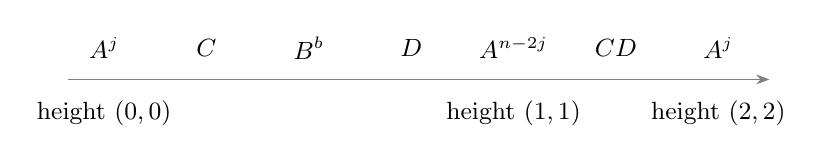
\begin{tikzpicture}[x=1.3cm,y=1cm,>=Stealth,font=\small]
\draw[->,gray] (-.35,0)--(6.5,0);
\node at (0,.4) {$A^j$};
\node at (1,.4) {$C$};
\node at (2,.4) {$B^b$};
\node at (3,.4) {$D$};
\node at (4,.4) {$A^{n-2j}$};
\node at (5,.4) {$CD$};
\node at (6,.4) {$A^j$};
\node[below,align=center] at (0,-.15) {height $(0,0)$};
\node[below,align=center] at (4,-.15) {height $(1,1)$};
\node[below,align=center] at (6,-.15) {height $(2,2)$};
\end{tikzpicture}
\end{center}
Only the leftmost $A$ block contributes to $K_{AB}$; the two outer block sizes must agree. This is the source of the arithmetic progression.

\subsection{The smallest displayed hole and a convexity consequence}
With $n=b=2$, all four letters occur twice and the exact $K_{AB}$ spectrum is $\{0,2\}$. Representatives are
\[
 \texttt{CBBDAACD}\quad(k=0),\qquad
 \texttt{ACBBDCDA}\quad(k=2).
\]
There is no representative with $k=1$ and the same other five pair counts. The claim here is a small explicit example, not a proof of global minimality by total word length.

\begin{corollary}[An integral hole in the convex hull]\label{gts:po:cor:convex}
For the fixed multiplicities $(2,2,2,2)$, the realizable complete pair profiles cannot be characterized by any conjunction of affine real inequalities and equalities in the six pair coordinates alone, followed only by restricting those coordinates to integers.
\end{corollary}
\begin{proof}
The feasible profiles with $k=0$ and $k=2$ and other coordinates $(2,2,2,4,3)$ have an integral midpoint with $k=1$. Every affine inequality or equality valid at both endpoints is valid at their midpoint. The midpoint is not realizable by Theorem~\ref{gts:po:thm:fourletter}. The argument even allows an infinite conjunction.
\end{proof}
This does not exclude nonlinear constraints, congruence conditions, auxiliary integer variables, or a disjunctive description. It pinpoints exactly why a convex pair-profile relaxation is insufficient.

\subsection{Why the ternary proof breaks}
With one separator species, a letter's order relative to the separators is encoded by a single height. Paired crossings preserve that one moment and can balance its distribution. With two separator species, an occurrence has a height vector, and fixing all other pair counts imposes several simultaneous restrictions. In~\eqref{gts:po:eq:skeleton}, the inequality $h_C\ge h_D$ and equality of their sums force every occurrence onto the diagonal heights. Transfers that would fill an intermediate $K_{AB}$ value leave that allowed diagonal. The new obstruction is not a loose endpoint estimate; the missing values are genuinely absent.

\section{Transfer to Heisenberg computational substrates}
\subsection{The collection identity with every orientation paid}
Use coordinates
\[
 h(\alpha,\beta,\gamma)=
 \begin{pmatrix}1&\alpha&\gamma\\0&1&\beta\\0&0&1\end{pmatrix},
 \qquad \alpha,\beta,\gamma\in\Z.
\]
Matrix multiplication gives
\begin{equation}\label{gts:po:eq:heisenberg}
 h(\alpha,\beta,\gamma)h(\alpha',\beta',\gamma')
 =h(\alpha+\alpha',\beta+\beta',
       \gamma+\gamma'+\alpha\beta').
\end{equation}
\wtagb\ This is the multiplication law~\eqref{gts:tp:eq:Hmult} of Section~\ref{gts:sec:heis} in source~06's Greek coordinates; it is kept here because this Part refers to it.
Fix three labelled generators $g_1,g_2,g_3\in\HH^r$. Equal group elements may carry different labels; multiplicities count labels. In factor $s$, their coordinates are $(\alpha_{si},\beta_{si},\gamma_{si})$, $i=1,2,3$. These are fixed signed integer coefficients, not nonnegative witnesses. For a word in the generators, let
\[
 (n_1,n_2,n_3)=(a,b,c),\qquad
 K_{12}=k,\quad K_{13}=p,\quad K_{23}=q.
\]
Define the reverse and diagonal pair counts by~\eqref{gts:po:eq:reverse}. If the target's factor-$s$ coordinates are $(A_s,B_s,C_s)$, repeated use of~\eqref{gts:po:eq:heisenberg} gives
\begin{align}
 A_s&=\sum_{i=1}^3\alpha_{si}n_i,\label{gts:po:eq:targetA}\\
 B_s&=\sum_{i=1}^3\beta_{si}n_i,\label{gts:po:eq:targetB}\\
 C_s&=\sum_{i=1}^3\gamma_{si}n_i+
            \sum_{i,j=1}^3\alpha_{si}\beta_{sj}K_{ij}.\label{gts:po:eq:targetC}
\end{align}
The cross term in a product records one contribution for every earlier/later pair of generator occurrences, which proves the last identity directly. No sorting of the actual word is assumed.

For a polynomial presentation, avoid divisions by setting
\[
 T_{ii}=n_i(n_i-1),\qquad T_{ij}=2K_{ij}\ (i<j),
 \qquad T_{ji}=2n_i n_j-2K_{ij}\ (i<j).
\]
Then the central equation is the quadratic residual
\begin{equation}\label{gts:po:eq:centralresidual}
 2C_s-\sum_i2\gamma_{si}n_i-
                  \sum_{i,j}\alpha_{si}\beta_{sj}T_{ij}=0.
\end{equation}
The horizontal equations are linear. Doubling the central coordinate is exact over the integers and introduces no witness.

\begin{theorem}[Profile-preserving matrix lift]\label{gts:po:thm:lift}
Fix $g_1,g_2,g_3\in\HH^r$ and externally fix $c\in\N$. A target $t\in\HH^r$ is the value of a word with prescribed statistics $(a,b,c;k,p,q)$ if and only if the gap certificate of Theorem~\ref{gts:po:thm:gapcompiler} and the $3r$ equations~\eqref{gts:po:eq:targetA}, \eqref{gts:po:eq:targetB}, \eqref{gts:po:eq:centralresidual} hold.

This is a certificate with $2c+4$ natural witnesses, $6+3r$ quadratic-or-linear residuals, and a quartic sum of squares. For $c=2$, the canonical profile certificate can instead be used, giving 24 natural witnesses and $24+3r$ residuals, with exactly one complete witness tuple for each accepted target-and-profile parameter tuple.
\end{theorem}
\begin{proof}
An actual word gives a valid pair profile and satisfies the collection identities, so it supplies a solution. Conversely, the profile certificate produces one actual word with all specified counts. The collection identities show that this word has exactly the target coordinates in every factor. Thus one common word, not a separate word for each factor, realizes the target.

All added residuals have degree at most two and use only the supplied profile statistics, fixed generator coefficients, and target coordinates. They add no auxiliary variables. For the canonical specialization, the profile witnesses are unique by Theorem~\ref{gts:po:thm:canonical}, and the matrix equations neither create nor multiply those witnesses.
\end{proof}

\subsection{Projection to target-only membership}\label{gts:po:sec:projection}
If the interface supplies only the target and requires exactly two occurrences of $g_3$, then $a,b,p,q,k$ become five additional natural witnesses. The gap specialization therefore gives 13 witnesses and $6+3r$ residuals; the canonical specialization gives 29 witnesses and $24+3r$ residuals. All remain quadratic systems and hence yield quartics.

The 29-witness target-only version need not be single-fold. Distinct realizable profiles can evaluate to the same group element, and every such profile has its own unique 24-tuple. This distinction between uniqueness \emph{over a profile} and uniqueness \emph{over a target} is essential.

The target coordinates may be signed integers, which is compatible with the natural witness convention: the polynomial parameters and fixed coefficients may be signed while its existentially quantified profile and gadget variables remain natural. The provided Python core implements the natural profile interface; the signed-target lift is specified and proved here, rather than advertised as a separate implemented exporter.

\subsection{A matrix substrate recording complete pair profiles}
There is a particularly transparent way to realize pair statistics as group coordinates. For an alphabet of $d\ge2$ letters, take one factor of $\HH$ for each unordered pair $i<j$. In that factor assign
\[
 g_i=h(1,0,0),\qquad g_j=h(0,1,0),
\]
and assign every other letter the identity. In the product over all $\binom d2$ factors, a word evaluates in factor $(i,j)$ to
\begin{equation}\label{gts:po:eq:recording}
 h(n_i,n_j,K_{ij}).
\end{equation}
This follows directly from~\eqref{gts:po:eq:heisenberg}. Consequently equality of these group products is exactly equality of complete pair profiles: the horizontal coordinates record the letter counts and the centers record all independent pair counts.

This map is not injective on words. It is injective on their pair-profile classes. For $d=3$ it realizes the interval theorem as a statement about central-coordinate slices of a fixed three-generator submonoid of $\HH^3$. For $d=4$, Theorem~\ref{gts:po:thm:fourletter} gives exact central-coordinate holes in a fixed four-generator submonoid of $\HH^6$. Thus the combinatorial obstruction has an explicit group-theoretic substrate and is not only a relaxation artifact in abstract statistics.

\wtagb\ In each factor this map is Part~I's area detector $a\mapsto h(1,0,0)$, $b\mapsto h(0,1,0)$ of~\eqref{gts:vk:eq:heisenberg}, applied to the positive word in two of the letters. On such words its central coordinate is the scattered pair count. It is not van Kampen area, for which Part~I uses the detector only as a lower bound, and it is not Part~II's coordinate $\lambda$. For an ordered binary alphabet the factor~\eqref{gts:po:eq:recording} is the Parikh matrix of the two-letter projection (Section~\ref{gts:po:sec:literature}).

In the cyclic three-factor presentation used by the repository, the central coordinates are $(K_{AB},K_{BC},K_{CA})=(k,q,ac-p)$. This is just a change of pair orientation; the same realizability theorem applies.

\section{Decidability with a supplied third multiplicity}
The certificate family separates one finite control parameter, $c$, from the potentially unbounded numbers of the other two generators. The following consequence makes that boundary precise.

\begin{theorem}[Supplied-multiplicity decision]\label{gts:po:thm:decidable}
Given a finite $r$, three integer Heisenberg tuples $g,h,j\in\HH^r$, a target $t\in\HH^r$, and a natural integer $c$, it is decidable whether a word over the three generator labels $g,h,j$ with exactly $c$ occurrences of $j$ evaluates to $t$. No bound on the numbers of $g$ and $h$ is supplied or required.
\end{theorem}
\begin{proof}
For each factor $s$, let
\[
 \Delta_s=\alpha_{sg}\beta_{sh}-\alpha_{sh}\beta_{sg}.
\]
First suppose some $\Delta_s\ne0$. Subtract the known horizontal contribution of $c$ occurrences of $j$ from that factor's target. The two remaining horizontal equations form a nonsingular $2\times2$ linear system for the multiplicities $a,b$ of $g,h$. Compute its unique rational solution and reject unless both values are natural. The possible pair counts now lie in finite ranges
\[
 0\le k\le ab,\qquad 0\le p\le ac,\qquad 0\le q\le bc.
\]
Enumerate these ranges. For each profile, finite gap enumeration decides realizability, and the collection equations check the target in every factor. This finite search is exact.

Now suppose every $\Delta_s=0$. Thus $g,h$ commute. For one factor define the injective integer-coordinate map
\begin{equation}\label{gts:po:eq:logcoords}
 \ellg h(\alpha,\beta,\gamma)=(2\alpha,2\beta,2\gamma-\alpha\beta).
\end{equation}
It is injective because the first two coordinates recover $\alpha,\beta$, after which the last recovers $\gamma$. For two elements of one Heisenberg factor, its central failure of additivity is
\[
 \alpha\beta'-\alpha'\beta.
\]
In particular, $\ellg(g^a)=a\ellg(g)$. For a full word, the central correction relative to the sum of the individual $\ellg$ coordinates is, in each factor,
\begin{equation}\label{gts:po:eq:logcorrection}
 \Delta_{gh}(2k-ab)+\Delta_{gj}(2p-ac)+\Delta_{hj}(2q-bc).
\end{equation}
The first term vanishes. Since $c$ is an already supplied integer, the remaining target equations in $a,b,p,q$ are linear. The exact constraints on the latter two statistics are simply
\[
 a,b,p,q\ge0,\qquad p\le ca,\qquad q\le cb.
\]
Every such $p,q$ is jointly realizable by the moment-fibre nonemptiness argument, and $k$ need not be specified because it has coefficient zero in every factor. Therefore the desired membership question is a finite system of integer linear equations and inequalities over nonnegative variables.

Introduce nonnegative slacks for the two inequalities and decide the resulting linear system by Lemma~\ref{gts:po:lem:linear}. Injectivity of~\eqref{gts:po:eq:logcoords} ensures that solving its equations is equivalent to the original group-coordinate equalities. Both branches terminate and are correct.
\end{proof}

\wtagb\ The map~\eqref{gts:po:eq:logcoords} is $(2\alpha,2\beta,\lambda)$ with Part~II's integral logarithmic coordinate $\lambda=2\gamma-\alpha\beta$, and~\eqref{gts:po:eq:logcorrection} is~\eqref{gts:tp:eq:loglaw} summed over the pairs of a word. This is the third independent derivation of that device in the repository, after the research note~\cite{repo-heis} (its Section~4) and Section~\ref{gts:tp:sec:two}. For $c=0$ the commuting branch is the note's commuting two-generator case, which in turn is the special case of Theorem~\ref{gts:tp:thm:two} with one generator in each phase and natural exponents.

\begin{lemma}[Elementary linear-feasibility algorithm]\label{gts:po:lem:linear}
For a given integer matrix $M$ and integer vector $d$, the existence of $z\in\N^s$ with $Mz=d$ is decidable.
\end{lemma}
\begin{proof}
Encode all coordinates of $z$ in base two, padding them to a common length and reading least-significant bits first. Start with carry vector $v_0=-d$. At each step choose a bit vector $b\in\{0,1\}^s$ and permit a transition precisely when every coordinate of $v+Mb$ is even; then set
\[
 v'=(v+Mb)/2.
\]
For row $i$, put $B_i=\max(|d_i|,\sum_j|M_{ij}|)$. The finite box $|v_i|\le B_i$ contains the initial state and is preserved by every transition. A path of length $t$ ending at zero gives
\[
 0=v_t=\frac{-d+M\sum_{u=0}^{t-1}2^u b_u}{2^t},
\]
so the finite bits yield a nonnegative solution. Conversely, the padded bits of any nonnegative solution give exactly such a path; all its intermediate carries are integral and remain in the box. Finite graph reachability from $-d$ to zero therefore decides the question. Empty paths cover the zero solution when appropriate.
\end{proof}

Theorem~\ref{gts:po:thm:decidable} is uniform in the supplied $c$, even though one branch may use very large finite searches. It does not decide the problem with an unrestricted existentially quantified $c$: searching all possible values of $c$ would not terminate on every negative instance. It also does not prove undecidable membership with only three generators; no such assertion is needed here.

\wtagb\ (2~October 2026.) With the interval theorem, Theorem~\ref{gts:po:thm:decidable} answers in part the question that the research note~\cite{repo-heis} leaves open and that Part~\ref{gts:part:tp} does not answer (Section~\ref{gts:sec:relation}): for three generators of a submonoid of $\HH^r$, word realizability is now paid exactly, and membership is decidable once the multiplicity of one generator is supplied. Whether three generators can give undecidable submonoid membership is not decided here (question~9 of Section~\ref{gts:po:sec:questions}).

\section{Executable verification and reproducibility}\label{gts:po:sec:software}
\subsection{Contents of the research package}
The package is self-contained apart from a standard LaTeX installation for rebuilding the PDF. The Python code requires Python 3.10 or later and uses only the standard library.
\begin{center}
\small
\begin{tabular}{p{.45\linewidth}p{.46\linewidth}}
\toprule
File & Purpose\\
\midrule
\code{article.tex}, \code{article.pdf} & This report and its editable source.\\
\code{code/pair_geometry.py} & Gap constructions, normalization paths, exact corner decision, polynomial gadgets, and quartic export.\\
\code{code/verify.py} & Independent finite checks and receipt replay.\\
\code{data/canonical_c2_quartic.json} & Complete residual list and expanded quartic.\\
\code{data/verification_receipt.json} & Recorded exact test counts and compiler-source digest.\\
\code{README.md}, \code{Makefile} & Build and execution instructions, interfaces, and limitations.\\
\bottomrule
\end{tabular}
\end{center}

Run from the package root:
\begin{lstlisting}
python3 code/verify.py
python3 code/pair_geometry.py decide 3 2 2 1 4
python3 code/pair_geometry.py export /tmp/canonical_c2_quartic.json
latexmk -pdf -interaction=nonstopmode article.tex
\end{lstlisting}
The second command accepts the worked profile and emits the complete natural witness tuple. Replacing the last argument by $1$ rejects it. Arguments are in the order $a,b,p,q,k$, with $c=2$ fixed by the command's interface.

\wtagb\ In this report the package is shipped under the prefix \path{06-pair-order-}: \path{code/06-pair-order-pair_geometry.py}, \path{code/06-pair-order-verify.py} and \path{code/06-pair-order-Makefile}, and \path{data/06-pair-order-canonical_c2_quartic.json}, \path{data/06-pair-order-verification_receipt.json} and \path{data/06-pair-order-worked_example.json}; the last, which the table above does not list, is the captured output of the command \texttt{decide 3 2 2 1 4}. Source~06's \path{article.tex}, \path{article.pdf}, \path{README.md} and checksum ledger are not shipped. The verifier imports the geometry module by its delivered name and finds the data through the delivered layout, and both \texttt{verify.py --write} and the Makefile's \texttt{export} target overwrite recorded files; run the programs only on a copy with the delivered layout (see the README). When the manuscript was placed, such a run passed in 59~seconds under Python~3.14.4, comparing every count with the bundled receipt, and the \texttt{decide} and \texttt{export} commands reproduced the two other data files apart from line endings.

\subsection{Independent profile enumeration}
The reference enumerator does not use the corner formula or gap constraints. It computes realizable triples $(k,p,q)$ by a last-letter recurrence. Appending $A$ creates no new forward-oriented pairs; appending $B$ adds the current number of $A$ letters to $k$; appending $C$ adds the current numbers of $A$ and $B$ to $p,q$. Starting from the empty word, this recurrence exhausts the profile set for each bounded multiplicity tuple.

For every resulting $(p,q)$ slice, the tests compare the full profile set with the union of all gap intervals, verify the no-holes property, and, when $c=2$, compare both endpoints with the four-corner formula. A separate enumeration of every ternary word of length at most eight checks the normalization path, including its invariant preservation and every change in $K_{AB}$.

\subsection{Recorded exact checks}
The bundled receipt records the following results:
\begin{center}
\small
\begin{tabular}{p{.65\linewidth}r}
\toprule
Check & Count\\
\midrule
Multiplicity boxes, $0\le a,b\le5$, $0\le c\le4$ &180\\
Nonempty ternary slices checked &8,730\\
Realizable profiles in those boxes &60,549\\
Two-separator endpoint checks &1,296\\
Ternary words in normalization-path tests, lengths $0$--$8$ &9,841\\
Normalization edges checked &22,619\\
Complete bounded profile decisions, including rejections &23,128\\
Accepted canonical witness samples &2,371\\
Rejected one-coordinate witness mutations &4,460\\
Signed off-zero expanded-polynomial checks &250\\
Independent direct $3\times3$ matrix products &2,000\\
Four-letter words with two of each letter &2,520\\
\bottomrule
\end{tabular}
\end{center}
The quartic tests also evaluate endpoint witnesses for inputs built from powers $10^{20}$, $10^{100}$, and $10^{300}$, without generating words of those lengths. The four-letter enumeration finds eight noninterval fibres for the displayed coordinate orientation in the all-two multiplicity box; the theorem uses one of them and proves its infinite extension. The repository's strict-interior false family is checked for $m=3,\ldots,99$.

These numbers describe finite computations, not the domains of validity of the theorems. In particular, single-foldness is proved by the triangular forcing argument, not by mutating a few witness coordinates. The tests do not exhaust all 24-dimensional candidate zero sets. Matrix comparisons check the collection formula independently of the scalar product routine, but do not instantiate a universal monoid or a halting reduction.

\subsection{Code boundaries and error handling}
Numeric input validators reject negative naturals, nonintegers, and Boolean values used as integers. Polynomial construction copies its input into an immutable canonical representation, preventing later mutation of an input list from changing a supposedly frozen expression.

The functions producing explicit words or enumerating gap vectors are intended for modest instances. They may take time proportional to large counts and may allocate long words. The two-separator decision command and canonical witness evaluation use exact big-integer arithmetic instead and do not enumerate words.

The compiler also permits evaluating polynomial residuals on signed arbitrary assignments for algebraic testing. Such an assignment is not a valid natural witness just because its residuals vanish. On rejected instances, the triangular candidate assignment may have a negative bound or endpoint slack; the natural-domain check is therefore part of the public decision procedure.

\section{Integration into ProveIt and further research}
\subsection{An incremental formalization route}
The most useful first formalization is the profile theorem, not a monolithic expansion of the quartic. A reasonable dependency chain is:
\begin{enumerate}[label=\arabic*.]
\item Define letter multiplicities and scattered pair counts on lists. Prove append formulas and the binary realization lemma.
\item Define gap decomposition and prove the total, moment, and cross-gap identities. Derive the six-equation soundness and completeness theorem.
\item Formalize paired crossings, potential descent, and the unique balanced gap vector. Prove the connectedness and interval theorems.
\item Verify the two-separator substitutions by polynomial normalization, then derive the corner criterion and canonical gadget uniqueness.
\item Add Heisenberg coordinates and prove the collection formula. Compose the profile and matrix certificates with a zero-set theorem for the sum of squares.
\end{enumerate}
Proposed modules might be named \code{WordPairProfile}, \code{TernaryGapRealization}, \code{TernaryPairInterval}, and \code{CanonicalTwoSeparator}. These are suggested names, not claims that such modules already exist or have been checked. The Python receipt is computational evidence; it is not a trusted Lean proof object.

A later compiler integration should produce explicit natural-to-positive coordinate maps, charge every subtraction and coefficient multiplication, and preserve the stated interface. The present construction intentionally separates polynomial degree, witness count, and runtime arithmetic count; optimizing one should not be reported as an improvement of another.

\subsection{Research questions with concrete next steps}\label{gts:po:sec:questions}
\paragraph{1. General endpoint complexity.}
Determine the bit complexity of evaluating~\eqref{gts:po:eq:generalendpoints} with binary-encoded $a,b,c,p,q$. The interval theorem removes internal membership gaps, but it leaves a structured bilinear optimization over integer moment fibres. A useful first target is an algorithm polynomial in $c$ and the bit lengths of $a,b,p,q$, rather than in the word length.

\paragraph{2. A closed formula for three separators.}
For $c=3$, each gap vector has two free coordinates after the total and moment equations are eliminated. Work out its integer polygon and determine whether finitely many residue-sensitive boundary candidates compute the extrema. The $c=2$ formula suggests a concrete test case for an arithmetic compiler more efficient than generic enumeration.

\paragraph{3. Small-support extremizers.}
Over real moment polytopes, linear objectives have sparse extremizers. Integer fibres can require additional support or residue corrections. Prove a correct support bound for a pair of extremizing integer gap vectors, or exhibit families ruling out an attractive constant bound. This could be the bridge from a separator-dependent compiler to a succinct all-$c$ endpoint description.

\paragraph{4. Uniform arity without hiding the separator count.}
Find a fixed-arity Diophantine certificate for the full ternary profile relation with $c$ as an ordinary parameter, accompanied by an explicit bound on witnesses and degree. General representability results alone would not supply the desired small construction or uniqueness. Encoding the gap list must be paid rather than treated as a variable-length primitive.

\paragraph{5. Canonical versus smallest certificates.}
Can the 24-witness endpoint construction be reduced while retaining uniqueness, especially on tied corners? Can both extrema share comparison work? A valid improvement should supply a complete zero-set bijection or a fresh triangular forcing proof, rather than discard apparently unused negative parts without checking all branches.

\paragraph{6. Succinct realizing words.}
The binary construction uses only a few runs. Determine whether every realizable ternary profile has a representative with a number of runs bounded independently of its multiplicities, or bounded by a useful function of $c$. A constructive result would convert the current decision certificate into a compact explicit word certificate. It would also clarify how our restricted invariants interact with group-theoretic bounded-generation results~\cite{po-shafrir}.

\paragraph{7. Classifying four-letter spectra.}
Theorem~\ref{gts:po:thm:fourletter} realizes pure arithmetic progressions. Which finite sets, unions of intervals, or residue patterns can occur when one pair count varies and all other counts are fixed? Seek structural restrictions before attempting a universal catalogue. The all-two enumeration provides a finite initial test set, not evidence of a complete classification.

\paragraph{8. Nonconvex profile constraints for matrix compilers.}
Corollary~\ref{gts:po:cor:convex} excludes affine constraints in the profile coordinates alone. Develop exact nonlinear or disjunctive constraints that detect separator-skeleton obstructions while keeping a manageable Diophantine interface. Compare their witness cost with simply supplying a gap decomposition.

\paragraph{9. Three-generator membership without a supplied multiplicity.}
Theorem~\ref{gts:po:thm:decidable} treats $c$ as input, not as an unbounded existential variable. Identify additional geometric conditions on three generators in $\HH^r$ that bound the necessary $c$, permit its elimination, or reduce the problem to a decidable arithmetic class. The present report does not assert that the unrestricted three-generator problem is currently open in every relevant formulation; its exact relation to existing classifications requires a dedicated literature audit.

\wtagb\ Part~\ref{gts:part:tp}'s three-subgroup theorem does not bear on this question: it concerns ordered products of subgroups or submonoids, with no interleaving of letters across phases (Section~\ref{gts:sec:relation}).

\paragraph{10. From profile existence to unambiguous target membership.}
Find generator families for which the target coordinates determine $(a,b,p,q,k)$ uniquely, so that the 24-witness single-fold property survives projection to targets. Conversely, characterize the affine and quadratic kernels responsible for multiple accepted profiles over one target. This question separates arithmetic witness ambiguity from word ambiguity.

\paragraph{11. Higher-step nilpotent groups.}
Upper-unitriangular matrices of larger size retain longer scattered subwords. Develop a version of the separator method for length-three counts and test whether connected-slice phenomena persist under a carefully specified collection of fixed invariants. The two-separator moment argument cannot simply be assumed to extend to those higher-order statistics.

\wtagb\ Compare Question~\ref{gts:vk:q:detectors} of Part~I and Section~\ref{gts:tp:q:nilpotent} of Part~II.

\paragraph{12. Counting profiles and connecting to sequence research.}
Let $N(a,b,c)$ count distinct ternary pair profiles. The interval theorem gives the exact identity
\[
 N(a,b,c)=\sum_{p=0}^{ac}\sum_{q=0}^{bc}
       \bigl(\up_c(a,b;p,q)-\low_c(a,b;p,q)+1\bigr).
\]
For $c=2$, substitute the corner expressions and seek piecewise quasipolynomial formulas, generating functions, and asymptotics along natural diagonals. This connects the current compiler problem to the repository's enumerative and asymptotic interests. No OEIS identification or asymptotic formula is claimed in this report.

\subsection{A precise boundary of the contribution}
The missing order relation is now completely characterized for ternary profiles, with an exact finite gap certificate for each separator count and a closed canonical quartic for the two-separator slice. The four-letter family proves a genuine failure of one-dimensional interval interpolation beyond that alphabet size. These statements are independent of any computational universality claim.

Nothing here instantiates Roman'kov's entire undecidable monoid, lowers the repository's advertised universal Diophantine-operation bound, or proves a global single-fold representation theorem for enumerable sets. The results are most useful as sound compiler components and as a sharply delimited account of what pair-count compression preserves, what it loses, and where further arithmetic work is needed.

\part{Affine matrix inputs (source 07)}\label{gts:part:ai}

\noindent\wtagb\ Part~IV prints batch-78 manuscript~13, \emph{Affine Matrix Inputs and Diophantine Universality: Sharp rigidity, exact period bounds, and computation with existential witnesses}, a research report prepared for Vladimir Reshetnikov, October~2, 2026; it names no author and is AI-assisted. Its labels carry the prefix \texttt{gts:ai:}. Its Section~$n$ is Section~$n+42$ here, and its Theorem~$n.m$ is Theorem~$(n+42).m$; it has no appendices. Like source~06 it was written from commit \texttt{4cccfa068} and could not know the other Parts. Its interpolation coordinates $\lambda_i$ are written $\theta_i$ (Section~\ref{gts:sec:notation}), and its automatic cross-references are printed with the statement type spelled out. Its abstract follows.

\begin{quote}\small
\textbf{Abstract (source 07).} A matrix subgroup can have an undecidable membership problem, but the way an ordinary integer input is loaded into that subgroup matters. We prove that, for every dimension $d$, every entrywise affine curve $L(n)=C+nD$ in $\SL_d(\Z)$, and every fixed subgroup $K$, the set of integers for which $L(n)\in K$ is either finite or exactly periodic. If $N=C^{-1}D$ has nilpotency index $k+1$, the finite case has at most $k$ elements, and every prescribed set of at most $k$ integers is realizable. A canonical free-abelian coordinate system gives the optimal universal period
\[
 P_k(e)=\prod_{p\mid e}p^{v_p(e)+\floor{\log_p k}},
\]
where $e$ is the exponent of the relevant finite lattice quotient. This extends the paired-$\SL_2$ obstruction in the audited \repo\ sources to arbitrary dimension. Combined with the repository's quadratic subgroup-input construction, it proves that input degree two is sharp even when the matrix dimension is unrestricted.

The obstruction changes completely when extra integer coordinates are existentially quantified. We give a six-dimensional, jointly affine, unimodular multiplication gadget with one uniquely determined auxiliary coordinate. It compiles a polynomial circuit with $g$ multiplication gates into membership in a fixed free-abelian unipotent subgroup of $\SL_{6g+2}(\Z)$, with exactly $2g$ uniquely determined added integer coordinates. The resulting certificate is an explicit quartic sum of squares. We also prove a commuting-polynomial extension, single-fold certificates for the rigid languages, a uniformity obstruction, and a one-witness decidability result for the block-cyclic model. The package includes an exact-arithmetic implementation and 91,142 finite verification cases. The results are developed as a repository-relative extension; global publication priority is not established, and no improved fixed universal-polynomial operation count or proof-assistant verification is claimed.
\end{quote}

\section{The research question and the source boundary}\label{gts:ai:sec:scope}
\subsection{What is being represented?}
A computational substrate is useful for Diophantine work only after its input convention, acceptance condition, and witnesses have been specified. The statement that a model is Turing-complete does not by itself give a small polynomial, a bounded number of variables, or a canonical certificate. In the present report the substrate is matrix subgroup membership. The first interface is
\begin{equation}\label{gts:ai:eq:interface}
 n\in S \quad\Longleftrightarrow\quad L(n)\in K,
\end{equation}
where $K$ is fixed, $n$ is the ordinary numerical input, and every entry of $L(n)$ is a prescribed polynomial in $n$. There are no additional input coordinates in this interface. Membership in $K$ may, of course, mean that some arbitrarily long word in its generators evaluates to $L(n)$. We do not count that word as a free arithmetic operation.

The second interface permits existential integer coordinates:
\begin{equation}\label{gts:ai:eq:quantified-interface}
 n\in S \quad\Longleftrightarrow\quad
 \exists\mathbf w\in\Z^m:\ \mathcal L(n,\mathbf w)\in K.
\end{equation}
Here $\mathcal L$ will be jointly affine in all its coordinates and unimodular for every assignment. The difference between \eqref{gts:ai:eq:interface} and \eqref{gts:ai:eq:quantified-interface} is decisive. An affine ordinary-input curve cannot recognize a nonrecursive set in any dimension, whereas a fixed affine pencil with finitely many existential coordinates can do so even when $K$ is abelian and its direct membership test is elementary.

Throughout, $\N=\{0,1,2,\ldots\}$, but the rigidity theorems use all of $\Z$. A set is \emph{exactly periodic} if it is a union of residue classes modulo some positive integer on all of $\Z$, not merely eventually periodic. Restriction to positive inputs is performed only after the classification. Integer and natural witnesses are kept distinct.

\subsection{What was already in ProveIt?}
The source audit was anchored to the repository revision
\begin{center}\small\texttt{4cccfa06866b6b81b2467e1cf7514ea85ed0216d}.\end{center}
The accompanying \texttt{SOURCE\_AUDIT.md} records the inspected paths and available blob hashes. Four source interfaces are important.

First, \emph{Affine paired-SL2 input cannot give universal subgroup membership} proves that one affine $\SL_2$ block, or two independently chosen such blocks, has a membership preimage that is empty, a singleton, or one full arithmetic progression \cite{ai-repoaffine}. The proof uses $N^2=0$. Its $\SL_3$ example realizes $\{1,2\}$, correctly showing that the stronger single-coset classification does not persist in higher dimension. It does not settle whether a weaker all-dimensional obstruction survives.

Second, \emph{An ordinary-input universal substrate from group commutators} constructs a fixed quadratic curve in $\SL_4(\Z)$ whose membership in a suitable finitely generated subgroup represents any given computably enumerable subset of the positive integers \cite{ai-repoquadratic}. Its group-theoretic upper bound is prior repository work, not a new universality construction in this report.

Third, the October 2 imported-substrate review distinguishes bounded certificates from one fixed polynomial handling unbounded computations, and distinguishes existence of witnesses from preservation of unique witnesses. It reports an 87-operation fixed universal-polynomial benchmark, but does not attribute such a bound to the matrix input loader \cite{ai-repoaudit}. We use that review as a scope constraint, not as a benchmark independently reverified here.

Finally, the repository contains an MRDP theorem whose polynomial and number of natural witnesses are independent of the input \cite{ai-repomrdp}. We invoke MRDP only when deriving the general computably enumerable consequence of our circuit compiler. The main affine rigidity theorem does not use MRDP.

\wtagb\ The repository already contained further material that source~07 does not list (Section~\ref{gts:sec:relation}): the research note~\cite{repo-unip}, whose curve source~07 reprints as $Q(n)$ in Section~\ref{gts:ai:sec:degree}; the complete matrix-membership compiler~\cite{repo-cmc}, which bears on question~10 of Section~\ref{gts:ai:sec:questions}; the programme's affine mortality notes, which load an affine input matrix as a semigroup generator for a zero-product problem, a different interface; and Part~VI of the report~\cite{pqc}, which prints Mihailova's generators. Part~\ref{gts:part:tp} of this report, written after source~07's pin, shows that the subgroup hypothesis of Theorem~\ref{gts:ai:thm:rigidity} cannot be dropped (Remark~\ref{gts:ai:rem:subgroup}). The four repository files cited above are unchanged from the pin to this write.

\subsection{Contribution and novelty status}
The principal extension is the all-dimensional finite-or-periodic theorem, strengthened by an exact free basis, a sharp finite-hit bound, and a sharp period formula. The explicit multiplication gadget and compiler explain a contrasting mechanism for Diophantine universality. They are not presented as a new proof of MRDP or as the discovery that multiplication can be encoded in unipotent matrices.

Integer-valued polynomials and polynomial sequences in groups have a substantial established theory \cite{ai-cahenchabert,ai-leibman,ai-hu}. Our proofs are elementary and self-contained at the points where the sharp bounds are obtained. The literature check did not establish whether an identical combination of statements has previously been published. Accordingly, ``new'' below means a result developed here beyond the inspected repository boundary, not a certified claim of global priority. Research questions in Section~\ref{gts:ai:sec:questions} are proposed continuation problems; none is advertised as a famous previously open conjecture solved here.

\section{Nilpotent normalization of an affine curve}\label{gts:ai:sec:normal}
\begin{lemma}[Affine unimodular normal form]\label{gts:ai:lem:normal}
Suppose $C,D\in M_d(\Z)$ and $\det(C+nD)=1$ for infinitely many integers $n$. Then $C\in\SL_d(\Z)$ and
\[
 L(n)=C(I+nN),\qquad N=C^{-1}D\in M_d(\Z),\qquad N^d=0.
\]
\end{lemma}
\begin{proof}
The polynomial $\det(C+tD)-1$ has infinitely many roots and is therefore zero. At $t=0$ this gives $\det C=1$, so $C^{-1}$ has integer entries. Consequently $\det(I+tN)=1$ identically. For an indeterminate $z$,
\[
 \det(zI-N)=z^d\det(I-z^{-1}N)=z^d.
\]
The identity may be read first in $\Q(z)$ and then in $\Q[z]$. Cayley--Hamilton gives $N^d=0$.
\end{proof}
If $N=0$, the hit set is either empty or all of $\Z$. Henceforth suppose $N\ne0$, and let $k+1$ be its nilpotency index. Thus
\begin{equation}\label{gts:ai:eq:index}
 N^{k+1}=0,\qquad N^k\ne0,\qquad 1\le k\le d-1.
\end{equation}
Set $U(n)=I+nN$. All the $U(n)$ commute, but they need not form a cyclic group: $U(s)U(t)=U(s+t)$ holds only when $N^2=0$. This is exactly why the old single-coset conclusion cannot simply be repeated in dimension three.

\begin{lemma}[Faithful truncated algebra]\label{gts:ai:lem:truncated}
The homomorphism
\[
 \Q[z]/(z^{k+1})\longrightarrow \Q[N],\qquad z\longmapsto N,
\]
is an isomorphism. On the nilpotent ideal $(z)$, the finite series $\log(1+x)$ and $\exp(x)$ are mutually inverse, and $\log(ab)=\log a+\log b$ for $a,b\in1+(z)$.
\end{lemma}
\begin{proof}
The minimal polynomial of $N$ is $z^{k+1}$. This proves the first assertion, including the linear independence of $N,N^2,\ldots,N^k$. The formal logarithm and exponential identities hold in $\Q[[z]]$ and descend modulo $z^{k+1}$, where every relevant sum is finite. The multiplicative identity uses commutativity, which holds in this algebra.
\end{proof}
In particular,
\begin{equation}\label{gts:ai:eq:logU}
 \log U(n)=\sum_{j=1}^k\frac{(-1)^{j+1}}j n^jN^j.
\end{equation}
Thus the logarithmic image of the affine matrix curve is an invertible linear image of the ordinary moment curve $(n,n^2,\ldots,n^k)$. The central issue is to retain its \emph{integral} lattice, rather than work only with its rational span.

\section{An exact free basis and canonical integer coordinates}\label{gts:ai:sec:basis}
For $1\le i\le k$ define the rational polynomial
\begin{equation}\label{gts:ai:eq:lambda}
 \theta_i(t)=\binom ti\binom{k-t}{k-i},\qquad
 \vv(t)=(\theta_1(t),\ldots,\theta_k(t))^{\mathsf T}.
\end{equation}
Binomial coefficients here mean their polynomial extensions. In particular, negative arguments are allowed. The identity
$\binom{-a}{j}=(-1)^j\binom{a+j-1}{j}$ for $a>0$ shows that each $\theta_i$ takes integer values on all integers.

\begin{lemma}[Integral interpolation]\label{gts:ai:lem:interpolation}
For every polynomial $f\in\Q[t]$ of degree at most $k$ with $f(0)=0$,
\begin{equation}\label{gts:ai:eq:interpolation}
 f(t)=\sum_{i=1}^k\theta_i(t)f(i).
\end{equation}
The polynomials $\theta_1,\ldots,\theta_k$ form a $\Z$-basis of the group of integer-valued polynomials of degree at most $k$ that vanish at zero.
\end{lemma}
\begin{proof}
At $t=j\in\{1,\ldots,k\}$ the value of $\theta_i$ is $\delta_{ij}$; at zero all are zero. Both sides of \eqref{gts:ai:eq:interpolation} have degree at most $k$ and agree at $k+1$ points. If $f$ is integer-valued, its coefficients in this interpolation basis are the integers $f(1),\ldots,f(k)$. Conversely every integer combination of the $\theta_i$ is integer-valued. Linear independence follows by evaluation at $1,\ldots,k$.
\end{proof}
\begin{theorem}[The affine evaluation lattice]\label{gts:ai:thm:freebasis}
Let
\[
 A_N=\langle I+nN:n\in\Z\rangle\le\SL_d(\Z).
\]
Then $A_N$ is free abelian of rank $k$, with basis
$U(1),U(2),\ldots,U(k)$. For every integer $n$,
\begin{equation}\label{gts:ai:eq:factorization}
 U(n)=\prod_{i=1}^k U(i)^{\theta_i(n)}.
\end{equation}
Thus the map $\Phi:\Z^k\to A_N$ defined by
$\Phi(a_1,\ldots,a_k)=\prod_iU(i)^{a_i}$ is an isomorphism and
$\Phi^{-1}(U(n))=\vv(n)$.
\end{theorem}
\begin{proof}
Apply Lemma~\ref{gts:ai:lem:interpolation} to the vector-valued polynomial \eqref{gts:ai:eq:logU}. It gives
$\log U(n)=\sum_i\theta_i(n)\log U(i)$. Exponentiating proves \eqref{gts:ai:eq:factorization}. The exponents are integers, so the assertion is genuinely about the group $A_N$, not a divisible enlargement of it.

The coefficient matrix of $\log U(1),\ldots,\log U(k)$ relative to $N,\ldots,N^k$ is obtained from $(i^j)_{1\le j,i\le k}$ by nonzero row rescalings. Its determinant is nonzero: factor $i$ from column $i$ and use the Vandermonde determinant on $1,\ldots,k$. Hence the logarithms are rationally independent. A relation $\prod_iU(i)^{a_i}=I$ therefore forces all $a_i=0$. Together with \eqref{gts:ai:eq:factorization}, this proves the theorem.
\end{proof}
The exact basis removes two possible ambiguities. The rank is the nilpotency index minus one, not necessarily the matrix dimension minus one. Also, no subgroup of $\Q^k$ with unbounded denominators is being introduced: every evaluation is in the explicit lattice generated by $k$ fixed matrices.

\begin{lemma}[Affine independence]\label{gts:ai:lem:moment}
Any $s\le k+1$ distinct points among $\vv(n)$, $n\in\Z$, are affinely independent.
\end{lemma}
\begin{proof}
The $\theta_i$ are a rational basis of the polynomials of degree at most $k$ with zero constant term. Thus $\vv(t)$ differs from $(t,t^2,\ldots,t^k)$ by an invertible linear transformation. The vectors $(1,n,n^2,\ldots,n^k)$ at $s$ distinct integers have rank $s$, since their first $s$ coordinates form a Vandermonde matrix. This is equivalent to affine independence.
\end{proof}

\section{The all-dimensional finite-or-periodic theorem}\label{gts:ai:sec:rigidity}
\begin{theorem}[Affine subgroup-input rigidity]\label{gts:ai:thm:rigidity}
Let $L(n)=C+nD\in\SL_d(\Z)$ for every integer $n$, and let $K\le\SL_d(\Z)$ be any subgroup. Set
\[
 T=\{n\in\Z:L(n)\in K\}.
\]
If $D=0$, then $T$ is empty or all of $\Z$. Otherwise let $k+1$ be the nilpotency index of $C^{-1}D$.

If $T\ne\varnothing$, choose $n_0\in T$, and let
\begin{equation}\label{gts:ai:eq:lattice}
 \Lambda=\Phi^{-1}(K\cap A_N)\le\Z^k,
 \qquad r=\rank\Lambda.
\end{equation}
Then
\begin{equation}\label{gts:ai:eq:cosetlattice}
 n\in T\quad\Longleftrightarrow\quad
 \vv(n)-\vv(n_0)\in\Lambda.
\end{equation}
If $r<k$, the set $T$ has at most $r+1$ elements. If $r=k$, it is exactly periodic. Consequently every $T$ is finite with at most $d-1$ elements, or is exactly periodic.
\end{theorem}
\begin{proof}
By Lemma~\ref{gts:ai:lem:normal}, $L(n)=CU(n)$. Since $L(n_0)\in K$, subgroup closure gives
\[
 L(n)\in K
 \ \Longleftrightarrow\ L(n_0)^{-1}L(n)\in K
 \ \Longleftrightarrow\ U(n_0)^{-1}U(n)\in K\cap A_N.
\]
The factor $C$ cancels in the indicated order; it is not moved across $U(n)$. Applying $\Phi^{-1}$ proves \eqref{gts:ai:eq:cosetlattice}.

When $r<k$, every point $\vv(n)$ with $n\in T$ belongs to the affine rational space $\vv(n_0)+\Span(\Lambda)$ of dimension $r$. If there were $r+2$ distinct such points, Lemma~\ref{gts:ai:lem:moment} would make them affinely independent, a contradiction.

When $r=k$, the quotient $\Z^k/\Lambda$ is finite. Let $e$ be its exponent, so $e\Z^k\subseteq\Lambda$. Each $\theta_i$ is integer-valued of degree at most $k$ and is periodic modulo $e$. For the latter fact, a crude direct bound is $e\,k!$: the polynomial $k!\theta_i$ has integer coefficients, so its value at $n+e k!$ minus its value at $n$ is divisible by $e k!$. Division by $k!$ shows that $\theta_i(n+e k!)\equiv\theta_i(n)\pmod e$. Thus \eqref{gts:ai:eq:cosetlattice} is unchanged by this positive shift. The sharp period bound is proved in Section~\ref{gts:ai:sec:period}.
\end{proof}
\begin{corollary}[No affine ordinary-input universality]\label{gts:ai:cor:noaffine}
For every fixed dimension, affine unimodular curve, and subgroup, the positive-input language \eqref{gts:ai:eq:interface} is recursive. No noncomputable computably enumerable set has such a representation, even if the dimension is allowed to vary when choosing the representation.
\end{corollary}
\begin{proof}
A finite set and a union of finitely many residue classes are recursive. This statement concerns each fixed set: it does not assert a uniform algorithm extracting its finite description from arbitrary subgroup generators. Such a uniform algorithm is impossible in general; see Section~\ref{gts:ai:sec:uniformity}.
\end{proof}
The theorem excludes more than undecidability. An infinite nonperiodic set, such as the positive squares, cannot occur. Indeed, an infinite periodic set has bounded gaps between successive sufficiently large elements, whereas the square gaps $2n+1$ are unbounded.

\begin{remark}[\wtagb\ The subgroup hypothesis is necessary]\label{gts:ai:rem:subgroup}
The proof of Theorem~\ref{gts:ai:thm:rigidity} uses closure of $K$ under $L(n_0)^{-1}L(n)$, and the conclusion fails for products of subgroups even on the simplest curves. In Theorem~\ref{gts:tp:thm:everyset} the hit set $\{n\in\N:g_0g_1^n\in\calA\calB\calT\}$ is an arbitrary prescribed c.e.\ set, where $\calA,\calB,\calT$ are free abelian subgroups of $\HH^d\le\SL_{3d}(\Z)$ and $g_1$ is central of infinite order. As a block-diagonal matrix, $g_1=I+E$ with $E$ a sum of matrix units in the corner positions of the diagonal blocks, so $E^2=0$, and $g_0g_1^n=g_0+n\,g_0E$ is an entrywise affine unimodular curve with $N=E$ square-zero: the case $k=1$. Hence, first, an ordered product of three free abelian subgroups, and by Corollary~\ref{gts:tp:cor:monoid} one of three free commutative submonoids, can have a nonrecursive hit set along an affine line, so Theorem~\ref{gts:ai:thm:rigidity} does not extend to such rational subsets; this answers the negative half of question~9 of Section~\ref{gts:ai:sec:questions} for three-factor products. Second, when the prescribed set is not recursive, $\calA\calB\calT$ is not a subgroup. For two commuting factors, Theorem~\ref{gts:tp:thm:two} reduces membership of $g_0g_1^n$ to an integer linear system whose right side depends polynomially on~$n$; whether hit sets of affine curves are then always finite or periodic is proved in neither Part and is left open.
\end{remark}

\section{The exact period formula}\label{gts:ai:sec:period}
The expression $\floor{\log_p k}$ below is the largest integer $b$ with $p^b\le k$. It is an integer definition and does not require floating-point logarithms.

\begin{definition}
For $k,e\ge1$, define
\begin{equation}\label{gts:ai:eq:period}
 P_k(e)=\prod_{p\mid e}p^{v_p(e)+\floor{\log_p k}}
       =e\prod_{p\mid e}p^{\floor{\log_p k}}.
\end{equation}
The empty product gives $P_k(1)=1$.
\end{definition}
\begin{lemma}[Newton basis]\label{gts:ai:lem:newton}
Every integer-valued $f\in\Q[t]$ of degree at most $k$ has a unique expansion
\[
 f(t)=\sum_{j=0}^k a_j\binom tj,\qquad a_j\in\Z.
\]
If $f(0)=0$, then $a_0=0$. Thus the bases
$(\theta_i)_{i=1}^k$ and $(\binom tj)_{j=1}^k$ are related by a unimodular integer change of coordinates.
\end{lemma}
\begin{proof}
Let $\Delta f(t)=f(t+1)-f(t)$. The identity
$\Delta\binom tj=\binom t{j-1}$ gives the Newton formula
$f(t)=\sum_{j=0}^k\Delta^j f(0)\binom tj$. It follows either by induction on degree or by agreement at $0,1,\ldots,k$. All finite differences are integers. Uniqueness follows from the different degrees. The last assertion follows because both families are $\Z$-bases of the same group, by Lemma~\ref{gts:ai:lem:interpolation}.
\end{proof}
\begin{lemma}[Simultaneous binomial divisibility]\label{gts:ai:lem:binomialperiod}
For $k,e\ge1$ and $n\in\Z$,
\begin{equation}\label{gts:ai:eq:kernel}
 e\mid\binom nj\text{ for every }1\le j\le k
 \quad\Longleftrightarrow\quad P_k(e)\mid n.
\end{equation}
\end{lemma}
\begin{proof}
The case $e=1$ is immediate. First take $n>0$, fix $p^a\Vert e$, and put $b=\floor{\log_p k}$.

For sufficiency suppose $v_p(n)\ge a+b$. The identity
$j\binom nj=n\binom{n-1}{j-1}$ gives
\[
 v_p\left(\binom nj\right)\ge v_p(n)-v_p(j)\ge a+b-b=a
\]
whenever the coefficient is nonzero; a zero coefficient is divisible by every power of $p$. This works for all $1\le j\le k$.

For necessity let $s=v_p(n)$. If $s\le b$, choose $j=p^s\le k$. For each $1\le\ell<p^s$ we have $v_p(n-\ell)=v_p(\ell)$. Consequently
\[
 \binom{n-1}{p^s-1}=\prod_{\ell=1}^{p^s-1}\frac{n-\ell}{\ell}
\]
is a $p$-adic unit. Since $v_p(n/p^s)=0$, the identity
$\binom n{p^s}=(n/p^s)\binom{n-1}{p^s-1}$ contradicts divisibility by $p$. Thus $s>b$. Applying the same argument with $j=p^b$ now gives
\[
 v_p\left(\binom n{p^b}\right)=s-b.
\]
Divisibility by $p^a$ forces $s\ge a+b$. Taking all primes dividing $e$ proves \eqref{gts:ai:eq:kernel} for positive $n$; $n=0$ is immediate.

For negative $n$, work in $(\Z/e\Z)[z]/(z^{k+1})$. The left side of \eqref{gts:ai:eq:kernel} says $(1+z)^n=1$ in this ring. The element $1+z$ is a unit, so this is equivalent to $(1+z)^{-n}=1$. The positive case applies to $-n$ and completes the proof.
\end{proof}
\begin{theorem}[Optimal universal period]\label{gts:ai:thm:period}
Every integer-valued polynomial of degree at most $k$ is periodic modulo $e$ with period $P_k(e)$. The vector $\vv(n)$ has least positive period $P_k(e)$ modulo $e$, and
\begin{equation}\label{gts:ai:eq:lambdakernel}
 \vv(n)\equiv0\pmod e\quad\Longleftrightarrow\quad P_k(e)\mid n.
\end{equation}
Consequently, in the full-rank case of Theorem~\ref{gts:ai:thm:rigidity}, $P_k(e)$ is a period of the hit set, where $e$ is the exponent of $\Z^k/\Lambda$.
\end{theorem}
\begin{proof}
Put $P=P_k(e)$. The binomial identity
\[
 \binom{n+P}{j}=\sum_{\ell=0}^j\binom P\ell\binom n{j-\ell}
\]
holds as a polynomial identity in $n$, including negative integers. By Lemma~\ref{gts:ai:lem:binomialperiod}, its terms with $\ell\ge1$ are divisible by $e$ for $j\le k$. Hence every Newton basis polynomial, and therefore every integer-valued polynomial of degree at most $k$, has period $P$ modulo $e$.

The unimodular basis change in Lemma~\ref{gts:ai:lem:newton} shows that $\vv(n)\equiv0\pmod e$ is equivalent to the simultaneous binomial divisibility condition. This proves \eqref{gts:ai:eq:lambdakernel}. If $q>0$ is any period of $\vv$ modulo $e$, then $\vv(q)=\vv(0)=0$ modulo $e$, so $P\mid q$. Since $P$ itself is a period, it is the least one. Finally $e\Z^k\subseteq\Lambda$ makes congruence modulo $e$ sufficient to preserve \eqref{gts:ai:eq:cosetlattice}.
\end{proof}
\begin{corollary}[Sharpness over all full-rank lattices]\label{gts:ai:cor:periodsharp}
For every $k,e\ge1$, let $N$ be a nilpotent Jordan block of size $k+1$, and let
\[
 K=\langle U(1)^e,\ldots,U(k)^e\rangle.
\]
Then $\{n:U(n)\in K\}=P_k(e)\Z$. In particular, no smaller universal period depending only on $k$ and $e$ can replace \eqref{gts:ai:eq:period}.
\end{corollary}
\begin{proof}
Here $\Lambda=e\Z^k$, whose quotient has exponent $e$. Apply \eqref{gts:ai:eq:lambdakernel}. The subgroup $P_k(e)\Z$ has least positive period $P_k(e)$.
\end{proof}
A bound such as $e\,\lcm(1,\ldots,k)$ is valid but can be wasteful: only primes already dividing $e$ need their additional powers. For example,
\[
 P_3(2)=4,\qquad P_8(12)=2^{2+3}3^{1+1}=288.
\]
The period of an individual hit set may be smaller than the universal bound; the sharpness assertion is a worst-case statement with fixed $k,e$.

\section{Sharp finite sets and diagnostic examples}\label{gts:ai:sec:examples}
\begin{theorem}[Every permitted finite set is realizable]\label{gts:ai:thm:finitesharp}
Fix $k\ge1$ and a nonempty finite set $F\subseteq\Z$ with $|F|\le k$. There exist an affine curve $L(n)\in\SL_{k+1}(\Z)$ and a finitely generated abelian subgroup $K$ such that
\[
 \{n\in\Z:L(n)\in K\}=F.
\]
The subgroup can be chosen of rank $|F|-1$.
\end{theorem}
\begin{proof}
Let $J$ be the nilpotent Jordan block of size $k+1$, put $U(n)=I+nJ$, and choose $n_0\in F$. Define
\[
 L(n)=U(n_0)^{-1}U(n),\qquad
 K=\langle U(n_0)^{-1}U(f):f\in F\setminus\{n_0\}\rangle.
\]
The inverse of $U(n_0)$ is an integral finite geometric series, so $L$ is an affine integral unimodular curve. Every element of $F$ is accepted. The vectors
$\vv(f)-\vv(n_0)$, $f\in F\setminus\{n_0\}$, are independent by Lemma~\ref{gts:ai:lem:moment}; hence $K$ has rank $|F|-1$. A further accepted integer would give $|F|+1\le k+1$ moment-curve points in an affine space of dimension $|F|-1$, contradicting the same lemma.
\end{proof}
This strengthens numerical sharpness: the finite exceptions can be placed at arbitrarily prescribed integers, not only at a convenient initial interval. For a fixed unshifted curve $U(n)$, however, zero is always accepted because every subgroup contains the identity. The translation by $U(n_0)^{-1}$ is therefore substantive.

\subsection{The square-zero case}
When $k=1$, we have $\theta_1(n)=n$. Every subgroup of $\Z$ is $a\Z$, and \eqref{gts:ai:eq:cosetlattice} gives an empty set, a singleton, or one coset $n_0+a\Z$. This recovers the exact conclusion of the paired-$\SL_2$ source \cite{ai-repoaffine}. The general theorem is not obtained by asserting that higher-dimensional affine curves are powers of one matrix; they usually are not.

\subsection{Dimension three: two points or two residue classes}
For $k=2$,
\begin{equation}\label{gts:ai:eq:k2coordinates}
 \theta_1(n)=n(2-n),\qquad \theta_2(n)=\frac{n(n-1)}2.
\end{equation}
Let $J=E_{12}+E_{23}$ and $U(n)=I+nJ$. The subgroup $\langle U(1)\rangle$ corresponds to $\Lambda=\Z(1,0)$, so its hit set is $\{0,1\}$. Replacing $U(n)$ by $U(n-1)$ yields $\{1,2\}$, the higher-dimensional boundary example in the repository.

There is also an infinite example that is not one coset. Let
\[
 K=\langle U(1),U(2)^2\rangle.
\]
Its lattice is $\Z\times2\Z$. Therefore
\[
 U(n)\in K
 \ \Longleftrightarrow\ \frac{n(n-1)}2\equiv0\pmod2
 \ \Longleftrightarrow\ n\equiv0\text{ or }1\pmod4.
\]
This set is exactly periodic but is not a coset of a subgroup of $\Z$. Both the finite and periodic alternatives in the all-dimensional theorem are genuinely broader than the old one-coset classification.

\subsection{Dimension four: a nonconsecutive sharp finite set}
For a Jordan block of size four, let $K=\langle U(2),U(5)\rangle$. Then
\[
 \{n:U(n)\in K\}=\{0,2,5\}.
\]
For an independent check, logarithmic coordinates relative to $J,J^2,J^3$ are $(n,-n^2/2,n^3/3)$. The linear functional $(v_1,v_2,v_3)\mapsto10v_1+14v_2+3v_3$ vanishes on both generator logarithms and has value
\[
 10n-7n^2+n^3=n(n-2)(n-5)
\]
on $\log U(n)$. Hence any accepted integer must be one of the three printed roots, all of which are indeed accepted. This avoids treating a finite search window as evidence for the unbounded assertion.

\section{Explicit Diophantine certificates for the rigid languages}\label{gts:ai:sec:certificates}
The classification can itself be compiled into a polynomial without MRDP, once the relevant lattice is supplied. This is useful as a certificate format, although the lattice need not be effectively recoverable from an arbitrary subgroup presentation.

\begin{theorem}[A single-fold lattice certificate]\label{gts:ai:thm:certificate}
In the nonconstant, nonempty situation of Theorem~\ref{gts:ai:thm:rigidity}, suppose an integer column basis
$B\in M_{k\times r}(\Z)$ of $\Lambda$ and an accepted input $n_0$ are given. Put
\[
 a_i(t)=k!\theta_i(t)\in\Z[t].
\]
Then the polynomial
\begin{equation}\label{gts:ai:eq:certificate}
 F(n,\mathbf y)=\sum_{i=1}^k
 \left(a_i(n)-a_i(n_0)-k!\sum_{j=1}^rB_{ij}y_j\right)^2
\end{equation}
has degree at most $2k$ and satisfies
\[
 L(n)\in K\quad\Longleftrightarrow\quad
 \exists\mathbf y\in\Z^r:\ F(n,\mathbf y)=0.
\]
For every accepted input, the integer witness tuple $\mathbf y$ is unique.
\end{theorem}
\begin{proof}
From the product expression in \eqref{gts:ai:eq:lambda}, multiplication by $k!$ clears its denominators: the remaining factor is $\binom ki$ times a product of integral linear factors. A sum of integer squares vanishes exactly when each summand vanishes. Dividing each residual equation by the nonzero integer $k!$ yields
$\vv(n)-\vv(n_0)=B\mathbf y$. This is equivalent to \eqref{gts:ai:eq:cosetlattice}. A column basis has independent columns, so the solution $\mathbf y$, when it exists, is unique. Each residual has degree at most $k$, giving the degree bound.
\end{proof}
For $r=0$, the sum over $j$ is empty and there are no witnesses. The empty language is represented by the constant polynomial $1$; the full language by $0$. These cases do not require choosing $n_0$ for an empty set.

\begin{corollary}[Canonical natural witnesses]\label{gts:ai:cor:natural}
The certificate in Theorem~\ref{gts:ai:thm:certificate} has a version with $2r$ natural witnesses, still unique over every accepted integer input, and degree at most $\max(2k,4)$.
\end{corollary}
\begin{proof}
Replace $y_j$ by $u_j-v_j$, with $u_j,v_j\in\N$, and add the squared residuals $(u_jv_j)^2$. Their vanishing forces $u_jv_j=0$. Every integer $y_j$ has exactly one such decomposition:
$u_j=\max(y_j,0)$ and $v_j=\max(-y_j,0)$. The resulting sum of squares has the stated degree and exact witness correspondence.
\end{proof}
This is a single-fold representation of a restricted class of recursive languages. It says nothing about whether arbitrary computably enumerable sets have finite-fold or single-fold Diophantine representations. Nor is the numerical witness bound a new universal-polynomial record: it applies precisely to languages already forced to be finite or periodic.

\subsection{A two-dimensional lattice example}
For the period-four example in Section~\ref{gts:ai:sec:examples}, take $n_0=0$ and $B=\diag(1,2)$. With $k=2$, \eqref{gts:ai:eq:certificate} becomes
\[
 \bigl(2n(2-n)-2y_1\bigr)^2+
 \bigl(n(n-1)-4y_2\bigr)^2=0.
\]
Its integer solution is unique when it exists, namely
$y_1=n(2-n)$ and $y_2=n(n-1)/4$. Existence is equivalent to $n\equiv0,1\pmod4$. This example exposes all coefficients and witnesses; there is no implicit matrix-word decoder.

\section{Why the classification is not a uniform decision algorithm}\label{gts:ai:sec:uniformity}
It is important to distinguish a theorem about the form of every fixed hit set from an algorithm computing that form from arbitrary subgroup data. Finitely generated subgroups of a direct product of two free groups can have undecidable membership; the fibre-product mechanism used in the repository and in the classical literature supplies such examples \cite{ai-bogopolski,ai-repoquadratic}.

\begin{proposition}[A nonconstant all-or-empty obstruction]\label{gts:ai:prop:uniform}
There is a fixed finitely generated subgroup $K'\le\SL_6(\Z)$ such that no algorithm, given the coefficients of an affine unimodular curve, always decides whether its hit set in $K'$ is empty. This remains true for a family of nonconstant curves whose hit sets are promised to be either empty or all of $\Z$.
\end{proposition}
\begin{proof}
Fix a finitely generated $K_0\le\SL_4(\Z)$ with undecidable membership, and let
\[
 E(t)=\begin{pmatrix}1&t\\0&1\end{pmatrix},\qquad
 K'=\{\diag(h,E(m)):h\in K_0,\ m\in\Z\}.
\]
For a supplied $C\in\SL_4(\Z)$, define
\[
 L_C(n)=\diag(C,E(n)).
\]
This is nonconstant and entrywise affine; its coefficient of $n$ has rank one. Every $E(n)$ lies in $\langle E(1)\rangle$, so
\[
 \{n:L_C(n)\in K'\}=
 \begin{cases}\Z,&C\in K_0,\\\varnothing,&C\notin K_0.\end{cases}
\]
An algorithm deciding which case holds would decide membership in $K_0$.
\end{proof}
In particular, Theorem~\ref{gts:ai:thm:certificate} is effective \emph{from an accepted point and an intersection-lattice basis}. It is not a claim that those data can always be extracted from arbitrary matrix generators. The ordinary input in the rigidity theorem is the varying scalar $n$, not the entries of the whole fixed matrix $C$. Confusing these two input conventions would incorrectly turn the classification into a solution of an undecidable problem.

\section{A commuting-polynomial extension}\label{gts:ai:sec:commuting}
Affinity forces all normalized coefficients to lie in the algebra generated by one nilpotent matrix. A related argument works for higher-degree matrix polynomials provided their normalized coefficient matrices commute.

\begin{theorem}[Commuting polynomial inputs]\label{gts:ai:thm:commuting}
Let
\[
 L(t)=C M(t),\qquad
 M(t)=I+\sum_{j=1}^{D}t^jA_j,
\]
where $C\in\SL_d(\Z)$, the matrices $A_j\in M_d(\Z)$ commute pairwise, and $\det M(t)=1$ identically. For every subgroup $K\le\SL_d(\Z)$, the hit set $T=\{n:L(n)\in K\}$ is finite or exactly periodic.

If $M$ is nonconstant, put $E=D(d-1)$. The finite case has at most $E$ elements. More precisely, $A=\langle M(n):n\in\Z\rangle$ is free abelian of some rank $h\le E$. In the nonempty case, if $K\cap A$ has full rank in $A$ and the quotient has exponent $e$, then $P_E(e)$ is a period of $T$. If the intersection has smaller rank, $|T|\le E$.
\end{theorem}
\begin{proof}
Commuting matrices over an algebraically closed field can be simultaneously upper triangularized. For completeness, find a common eigenvector by restricting successive commuting operators to an eigenspace of a preceding one; these restrictions preserve that eigenspace. Induction on the quotient dimension then gives a common triangular basis.

In this basis, the diagonal entries of $M(t)$ are scalar polynomials with constant term one. Their product is the constant polynomial one. Since a polynomial ring over a field has no nonconstant units, each diagonal polynomial is one. Thus each $A_j$ is strictly upper triangular in the common basis. Every product of $d$ such matrices is zero. Consequently the commutative algebra without identity generated by the $A_j$ is nilpotent of index at most $d$.

The finite logarithm
\[
 f(t)=\log M(t)=\sum_{\ell=1}^{d-1}
 \frac{(-1)^{\ell+1}}\ell\bigl(M(t)-I\bigr)^\ell
\]
is a matrix-valued rational polynomial of degree at most $E$ and has $f(0)=0$. By integral interpolation, its integer evaluations generate the same additive group as the finite list $f(1),\ldots,f(E)$. All their entries are rational. That generated group is finitely generated and torsion-free, hence free abelian, of rank $h\le E$. Logarithm and exponential identify it with $A$.

Choose an abstract integer basis of this additive group and express $f(t)$ in its coordinates. The resulting vector $\mathbf F(t)\in\Q[t]^h$ has degree at most $E$, vanishes at zero, takes values in $\Z^h$ at integers, and its integer evaluations span $\Q^h$. If $n_0$ is accepted, cancellation as in Theorem~\ref{gts:ai:thm:rigidity} gives a lattice $\Lambda\le\Z^h$ with
\[
 n\in T\quad\Longleftrightarrow\quad
 \mathbf F(n)-\mathbf F(n_0)\in\Lambda.
\]
For full-rank $\Lambda$, each coordinate is periodic modulo the quotient exponent $e$ with period $P_E(e)$, by Theorem~\ref{gts:ai:thm:period} and the Newton basis proof.

If $\rank\Lambda<h$, choose a nonzero rational linear functional $\ell$ annihilating $\Lambda$. Every accepted $n$ is a root of
$q(t)=\ell(\mathbf F(t)-\mathbf F(n_0))$. This polynomial is not identically zero: otherwise evaluation at zero first gives $\ell(\mathbf F(n_0))=0$, and then $\ell$ vanishes on all evaluations of $\mathbf F$, contradicting their spanning property. Hence $q$ has at most $E$ roots.
\end{proof}
The affine case has the stronger rank-sensitive finite bound $r+1$ because its logarithmic curve is a full moment curve. An arbitrary commuting-polynomial curve can have algebraic dependencies, so the proof above uses the degree of a separating scalar polynomial instead.

The hypothesis is \emph{pairwise commutativity of the normalized coefficients}. It must not be replaced by the assertion that every individual evaluated matrix is unipotent. A family of unipotent matrices can vary through noncommuting directions. The quadratic universal curves in the next section do exactly this.

\section{Input degree two is sharp, even with unrestricted dimension}\label{gts:ai:sec:degree}
\subsection{The upper bound is prior repository work}
The following upper bound is the group-commutator construction already present in \repo\ \cite{ai-repoquadratic}. We reconstruct its mathematical interfaces because the conclusion about a sharp threshold depends on more than a bare statement that some matrix membership problem is undecidable. The proof uses the effective form of Higman's embedding theorem \cite{ai-higman,ai-mikaelian}. It does not instantiate a particular universal finite presentation or provide a fixed-size Diophantine checker for arbitrary matrix words.

\begin{theorem}[Quadratic upper bound; repository construction]\label{gts:ai:thm:quadratic}
There is a fixed degree-two curve $\Gamma:\Z\to\SL_4(\Z)$ such that, for each computably enumerable $S\subseteq\Z_{>0}$, one can construct a finitely generated subgroup $K_S$ with
\[
 n\in S\quad\Longleftrightarrow\quad \Gamma(n)\in K_S
 \qquad(n>0).
\]
One choice is $\Gamma(n)=\diag(R(n),R(n))$, where, with $t=4n-1$,
\begin{equation}\label{gts:ai:eq:quadraticR}
 R(n)=\begin{pmatrix}1-4t&-16\\t^2&1+4t\end{pmatrix}.
\end{equation}
\end{theorem}
\begin{proof}
We separate four steps so that the input curve is not confused with the quotient group in which the computation is encoded.

\paragraph{Step 1: an exact recursively presented group.}
Write $[g,h]=ghg^{-1}h^{-1}$, $a_i=b^{-i}ab^i$, and
\[
 G_S=\langle a,b\mid[a_n,a_0]=1\text{ for }n\in S\rangle.
\]
Consider also the graph group on generators $c_i$, $i\in\Z$, with a commuting relation between $c_i,c_j$ exactly when $|i-j|\in S$. Translation of the indices defines an automorphism. Adjoining a stable generator $b$ with $b^{-1}c_i b=c_{i+1}$ gives a semidirect product in which the graph group embeds. Eliminating all $c_i$ except $c_0$ gives the presentation of $G_S$, with $a=c_0$.

If $n\in S$, the commutator $[a_n,a_0]$ is a defining relation. If $n>0$ and $n\notin S$, map $c_n,c_0$ to the two free generators of $F_2$ and every other $c_i$ to the identity. Every graph relation is respected, since the only pair that could fail to commute is the missing edge. The image of $[c_n,c_0]$ is a nontrivial reduced free commutator. Thus
\begin{equation}\label{gts:ai:eq:commutatorcoding}
 [a_n,a]=1\text{ in }G_S\quad\Longleftrightarrow\quad n\in S.
\end{equation}
The positive-input convention excludes $n=0$, whose commutator is always trivial.

\paragraph{Step 2: a finite presentation with named free letters.}
An enumerator for $S$ enumerates the relators of $G_S$. Effective Higman embedding gives a finitely presented group $H_0$ and an injective homomorphism $G_S\hookrightarrow H_0$, together with words for the images of $a,b$ \cite{ai-higman,ai-mikaelian}. Adjoin fresh presentation letters named $a,b$ and relations identifying them with these image words. The resulting finite presentation $H$ still contains $G_S$ injectively. Its ambient free group $F$ has finitely many basis letters, two of them the named $a,b$.

The distinction is essential: $a,b$ are independent letters in $F$, though their images in the quotient $H$ may satisfy relations. A faithful matrix representation is assigned to $F$, not directly to $H$. No bound on the number of presentation letters is needed for the matrix curve below.

\paragraph{Step 3: a fibre-product subgroup.}
Let $H=F/\langle\!\langle R_1,\ldots,R_m\rangle\!\rangle$ and set
\[
 M(H)=\{(u,v)\in F\times F:u=v\text{ in }H\}.
\]
This subgroup is generated by $(z,z)$ for the finitely many free basis letters $z$, together with $(1,R_j)$ for $1\le j\le m$. \wtagb\ (This is Proposition \texttt{pqc:dr:prop:mihailova} of~\cite{pqc}, also its Lemma \texttt{pqc:rr:lem:mihailova} and Section~3 of~\cite{repo-comm}; the verification that follows is source~07's, printed as a second route.) Indeed, if $u^{-1}v$ is a product of conjugates $gR_j^{\pm1}g^{-1}$, each factor is represented by
\[
 (1,gR_j^{\pm1}g^{-1})=(g,g)(1,R_j)^{\pm1}(g,g)^{-1},
\]
and multiplication after $(u,u)$ gives $(u,v)$. This is the usual Mihailova fibre-product mechanism \cite{ai-bogopolski}.

Conjugate once by $(a,1)$:
\[
 M_a=(a,1)M(H)(a^{-1},1).
\]
Then
\begin{align*}
 (a_n,a_n)\in M_a
 &\Longleftrightarrow (a^{-1}a_n a,a_n)\in M(H)\\
 &\Longleftrightarrow a^{-1}a_n a=a_n\text{ in }H\\
 &\Longleftrightarrow [a_n,a]=1\text{ in }H\\
 &\Longleftrightarrow n\in S.
\end{align*}
Injectivity of the embedding in Step 2 is what justifies the last equivalence.

\paragraph{Step 4: a faithful fixed matrix input.}
Let
\[
 V=\begin{pmatrix}1&4\\0&1\end{pmatrix},\qquad
 B=\begin{pmatrix}1&0\\1&1\end{pmatrix}.
\]
These matrices freely generate a rank-two free group. One elementary verification starts with the matrices having off-diagonal entries $2,2$. On the real projective line, nonzero powers of the upper shear send $|x|<1$ into $|x|>1$, and nonzero powers of the lower shear send $|x|>1$ into $|x|<1$. The ping-pong argument proves freeness. Conjugating by $\diag(2,1)$ changes the off-diagonal entries to $4,1$ and preserves freeness. This is a standard free-matrix construction; see also \cite{ai-chang}.

In the free group on $V,B$, the elements $V^iBV^{-i}$ at distinct integer indices are freely independent. To check this directly, combine adjacent occurrences with the same index. A nonempty reduced word in the remaining conjugates has the form
\[
 V^{i_1}B^{e_1}V^{i_2-i_1}B^{e_2}\cdots
 V^{i_s-i_{s-1}}B^{e_s}V^{-i_s},
\]
with nonzero $e_j$ and distinct adjacent indices. Its internal alternating blocks cannot cancel, so it is nontrivial.

Assign the free basis letter $b$ to $B$, $a$ to
\[
 A=VBV^{-1}=\begin{pmatrix}5&-16\\1&-3\end{pmatrix},
\]
and any remaining letters to distinct $V^iBV^{-i}$ with $i\ge2$. This gives a faithful representation $\rho:F\hookrightarrow\SL_2(\Z)$ for every finite rank, with the same images of $a,b$. A direct multiplication gives
\[
 \rho(a_n)=B^{-n}AB^n=R(n)
\]
with $R$ as in \eqref{gts:ai:eq:quadraticR}. The image of $M_a$ under the faithful block-diagonal map
$(u,v)\mapsto\diag(\rho(u),\rho(v))$ is the required finitely generated subgroup $K_S$. All its generators are computable from the finite presentation, while the displayed curve is independent of $S$.
\end{proof}
The two-generator-output refinement of effective Higman embedding is not needed in this reconstruction. It would permit a different convenient finite-rank embedding, but the infinite free family in Step 4 already handles arbitrary finite presentation rank.

\wtagb\ Theorem~\ref{gts:ai:thm:quadratic} and its proof reconstruct Sections~1--4 of the research note~\cite{repo-comm}, as source~07 says; the theorem is not a result of this report. Step~4 also re-derives the free pair and conjugate family of~\cite{repo-unip} (its Section~1).

\begin{corollary}[Sharp degree threshold]\label{gts:ai:cor:degree}
Among ordinary-input representations \eqref{gts:ai:eq:interface} with integral unimodular matrix curves and a fixed finitely generated subgroup, the least possible entrywise polynomial degree capable of representing a noncomputable computably enumerable set is two. This remains true when the matrix dimension is unrestricted; degree two suffices in dimension four.
\end{corollary}
\begin{proof}
Degree zero or one is ruled out in every dimension by Corollary~\ref{gts:ai:cor:noaffine}. Degree two is supplied by Theorem~\ref{gts:ai:thm:quadratic} after choosing a noncomputable computably enumerable $S$.
\end{proof}
This is a lower bound on \emph{input degree in a specified subgroup interface}. It is not a lower bound on the degree of Diophantine polynomials, arithmetic operations, number of witnesses, or matrix dimension for other computational interfaces.

\subsection{Pointwise unipotence is not enough}
The same repository gives another quadratic loader,
\begin{equation}\label{gts:ai:eq:Q}
 Q(n)=\begin{pmatrix}1+12n&1\\-144n^2&1-12n\end{pmatrix}.
\end{equation}
\wtagb\ This curve is $L_*(x)$, equation~(12) of the research note~\cite{repo-unip}, with $c=12$; it is also printed in~\cite{repo-comm}. Source~07 does not cite the former note.
Every evaluated matrix satisfies $\det Q(n)=1$, $\tr Q(n)=2$, and $(Q(n)-I)^2=0$. Nevertheless its normalized coefficient matrices do not commute. In fact
\[
 Q(0)^{-1}Q(n)=I+nX+n^2Y,
\]
where
\[
 X=\begin{pmatrix}12&12\\0&-12\end{pmatrix},\qquad
 Y=\begin{pmatrix}144&0\\-144&0\end{pmatrix}.
\]
For example $(XY)_{11}=0$ but $(YX)_{11}=1728$. Thus Theorem~\ref{gts:ai:thm:commuting} does not apply. A restriction stated merely as ``unipotent matrix inputs'' would not express the required obstruction.

\section{Multiplication inside a jointly affine abelian pencil}\label{gts:ai:sec:gadget}
The negative theorem does not survive unrestricted existential coordinates. The following small construction makes the reason explicit.

Let
\[
 J=E_{12}+E_{23},\qquad P=I+J,
 \qquad B(t)=\binom t2=\frac{t(t-1)}2,
\]
and define a jointly affine matrix pencil
\begin{equation}\label{gts:ai:eq:T}
 T(t,s)=I+tJ+sJ^2=
 \begin{pmatrix}1&t&s\\0&1&t\\0&0&1\end{pmatrix}.
\end{equation}
It is an integer unimodular matrix for every integer assignment, and
\begin{equation}\label{gts:ai:eq:Ppowers}
 P^m=I+mJ+B(m)J^2\qquad(m\in\Z).
\end{equation}
The binomial identity for negative powers follows either from the finite nilpotent expansion or by checking the multiplication law and inverse. The entry $(1,2)$ makes the exponent unique. Consequently
\begin{equation}\label{gts:ai:eq:triangularmembership}
 T(t,s)\in\langle P\rangle\quad\Longleftrightarrow\quad s=B(t).
\end{equation}
Here subgroup membership is easy: it is one quadratic equality. The computational effect will come from existentially choosing coordinates that must satisfy many such equalities together.

\begin{theorem}[Six-dimensional multiplication with one auxiliary]\label{gts:ai:thm:mul}
For all integers $x,y,z,u$,
\begin{equation}\label{gts:ai:eq:mulblock}
 \diag\bigl(T(x+y,u),T(x-y,u-2z+y)\bigr)
 \in\langle P\rangle\times\langle P\rangle
\end{equation}
holds if and only if
\[
 z=xy\quad\text{and}\quad u=B(x+y).
\]
The matrix in \eqref{gts:ai:eq:mulblock} is jointly affine in $x,y,z,u$, lies in $\SL_6(\Z)$ for every assignment, and has exactly one auxiliary solution $u$ for every true multiplication triple $(x,y,xy)$.
\end{theorem}
\begin{proof}
By \eqref{gts:ai:eq:triangularmembership}, membership is equivalent to
\[
 u=B(x+y),\qquad u-2z+y=B(x-y).
\]
The identity
\begin{equation}\label{gts:ai:eq:polarization}
 B(x+y)-B(x-y)=2xy-y
\end{equation}
turns their difference into $2z=2xy$. Conversely, if $z=xy$ and $u=B(x+y)$, \eqref{gts:ai:eq:polarization} gives the second equation. All matrix entries in \eqref{gts:ai:eq:mulblock} are affine expressions. Both blocks have determinant one for every assignment, not just on their zero set. Uniqueness of $u$ follows from the first equation.
\end{proof}
The auxiliary $u$ is nonnegative even for signed $x,y$, because $B(t)\ge0$ for every integer $t$. No nonnegativity assumption is needed for the other variables or for the two cyclic exponents.

\begin{remark}[\wtagb\ The binomial device of Part~II]\label{gts:ai:rem:binomial}
In the coordinates of Section~\ref{gts:sec:heis}, $T(t,s)=h(t,t,s)$ and $P=h(1,1,0)$, so~\eqref{gts:ai:eq:triangularmembership} says that $h(t,t,s)$ lies in $\langle h(1,1,0)\rangle$ exactly when $s=\bn(t)$. Part~\ref{gts:part:tp}'s third phase uses the same binomial term in another cyclic subgroup, $\langle h(-1,-1,0)\rangle$ (equation~\eqref{gts:tp:eq:T}); the two subgroups differ, since $h(1,1,0)^{-1}=h(-1,-1,1)$. The polarizations differ as well: \eqref{gts:ai:eq:polarization} here, $st=\bn(s+t)-\bn(s)-\bn(t)$ in~\eqref{gts:tp:eq:polar}. So do the mechanisms. Part~II puts the existential witnesses into the exponents of three commutative phases and keeps the target on a fixed central line; Part~IV puts them into the target coordinates of a jointly affine pencil tested against one fixed free abelian subgroup $\langle P\rangle^{2g}\times\{I_2\}$. Part~II had already shown that commutative unipotent data can carry universal existential arithmetic (Theorem~\ref{gts:tp:thm:main}); source~07, which could not know that Part, reaches the same conclusion independently in Corollary~\ref{gts:ai:cor:abuniversality}, and its Proposition~\ref{gts:ai:prop:onewitness} plays the role of Part~II's phase threshold for its own resource, the number of quantified coordinates.
\end{remark}

\subsection{A literal quartic certificate}
Define the quadratic residuals
\begin{align}
 R_1&=2u-(x+y)(x+y-1),\label{gts:ai:eq:R1}\\
 R_2&=2(u-2z+y)-(x-y)(x-y-1).\label{gts:ai:eq:R2}
\end{align}
Then
\begin{equation}\label{gts:ai:eq:difference}
 R_1-R_2=4(z-xy).
\end{equation}
Thus the single polynomial $R_1^2+R_2^2$ vanishes over the integers precisely on the complete witness graph in Theorem~\ref{gts:ai:thm:mul}. Its degree is at most four. The identity also provides a simple corruption diagnostic: changing the product coordinate while retaining the two residual equations is impossible.

There is no assertion that dimension six or one auxiliary is optimal under every possible matrix encoding. These are explicit achieved bounds for this particular jointly affine, independent-block construction. The use of two different affine arguments, $x+y$ and $x-y$, is what recovers their product while leaving all matrix entries affine.

\section{A witness-preserving circuit compiler}\label{gts:ai:sec:compiler}
\subsection{The source format and the charged resources}
Take an integer polynomial given by a straight-line arithmetic circuit using addition, subtraction, integer constants, and multiplication. Absorb every purely affine computation between multiplication gates into the operands of the next such gate. After ordering the multiplication gates topologically, the source has the form
\begin{equation}\label{gts:ai:eq:circuit}
 z_i=A_i(\mathbf v,z_1,\ldots,z_{i-1})
     B_i(\mathbf v,z_1,\ldots,z_{i-1}),\qquad 1\le i\le g,
\end{equation}
with final output $A_0(\mathbf v,\mathbf z)$, where all $A_i,B_i,A_0$ are integral affine forms. This normalization is an algebraic reorganization, not a claim that large coefficients or long affine forms have zero implementation cost. The parameter $g$ counts multiplication gates only, and the resulting coefficient sizes still belong to the output data.

For each gate, introduce one additional coordinate $u_i$. Its two blocks are
\begin{equation}\label{gts:ai:eq:gateblocks}
 T(A_i+B_i,u_i),\qquad
 T(A_i-B_i,u_i-2z_i+B_i).
\end{equation}
Append the two-dimensional block $E(A_0)$ from Section~\ref{gts:ai:sec:uniformity}. Define
\begin{equation}\label{gts:ai:eq:Kg}
 K_g=\langle P\rangle^{2g}\times\{I_2\}
       \le\SL_{6g+2}(\Z).
\end{equation}
Each cyclic factor occupies its own three-dimensional diagonal block. This is a fixed free-abelian subgroup of rank $2g$, depending only on $g$, not on the coefficients of the source polynomial or on its input.

\begin{theorem}[Affine abelian compiler]\label{gts:ai:thm:compiler}
For the source circuit \eqref{gts:ai:eq:circuit}, let $\mathcal L(\mathbf v,\mathbf z,\mathbf u)$ be the block diagonal matrix consisting of \eqref{gts:ai:eq:gateblocks} for all gates and the final block $E(A_0)$. Then:
\begin{enumerate}[label=\textnormal{(\roman*)}]
\item $\mathcal L$ is jointly affine in every source, register, and auxiliary coordinate, and is in $\SL_{6g+2}(\Z)$ for every integer assignment.
\item For every fixed source tuple $\mathbf v$, the source polynomial vanishes if and only if there exist $\mathbf z,\mathbf u\in\Z^g$ with $\mathcal L(\mathbf v,\mathbf z,\mathbf u)\in K_g$.
\item Whenever the source polynomial vanishes, this tuple of $2g$ added integer coordinates is unique.
\item All normalized coefficient matrices of $\mathcal L$ commute. An explicit quartic sum of squares defines precisely the same integer witness set.
\end{enumerate}
\end{theorem}
\begin{proof}
All entries in \eqref{gts:ai:eq:gateblocks} and $E(A_0)$ are affine combinations of the coordinates. Each diagonal block is upper triangular with diagonal entries one, so the determinant of the entire matrix is one identically.

By Theorem~\ref{gts:ai:thm:mul}, membership of gate $i$ in its two cyclic factors is equivalent to the multiplication equation in \eqref{gts:ai:eq:circuit}, together with
\[
 u_i=B(A_i+B_i).
\]
Because $A_i,B_i$ depend only on source coordinates and earlier registers, induction on $i$ shows that all $z_i$ are exactly the source circuit values and are uniquely determined. The $u_i$ are then uniquely determined too. The last block belongs to $\{I_2\}$ precisely when $A_0=0$. This proves the equivalence and uniqueness.

Within a three-dimensional block, every matrix is a polynomial in the same $J$ of degree at most two; within the last block every matrix is a polynomial in $E_{12}$ of degree at most one. Different blocks commute. The constant block matrix is invertible in this same commutative algebra, so multiplying by its inverse to normalize the constant term preserves coefficient commutativity.

For the polynomial certificate, take $A_0^2$ plus the squares of the two residuals \eqref{gts:ai:eq:R1}--\eqref{gts:ai:eq:R2} with $(x,y,z,u)=(A_i,B_i,z_i,u_i)$ for each gate. As the operands are affine in the full coordinate list, all gate residuals are quadratic. Their squared sum is an integral polynomial of degree at most four, and zero exactly when every block has the required membership.
\end{proof}
The compiler preserves the source witness set by a bijection after adjoining its uniquely determined computational coordinates. It does not reduce the number of original solutions of the source equation. The group-word exponents are also determined by the displayed first-superdiagonal entries, so this construction does not hide uncontrolled word multiplicities inside an undecidable membership oracle.

\subsection{A precise resource ledger}
If the source has $m$ existential integer coordinates and $g$ multiplication gates, the output uses $m+2g$ existential integer coordinates and dimension $6g+2$. It has $2g$ independent cyclic subgroup generators and $2g+1$ residual equations, combined into one quartic polynomial. The matrix itself has $6g+2$ diagonal entries equal to one and only a linear number of nonconstant off-diagonal positions.

These are structural counts, not a total arithmetic-operation count for evaluating the final polynomial. Expanding long affine forms can increase that count, as can converting natural domains to integer domains. Neither the six-dimensional multiplication gadget nor the dimension formula is a comparison with the repository's fixed universal-polynomial operation benchmark.

\wtagb\ (2~October 2026.) The research programme's review of this manuscript~\cite{repo-revaffine} confirms Theorems~\ref{gts:ai:thm:mul} and~\ref{gts:ai:thm:compiler} and proves a reduction for square gates. For a gate $z=x^2$ the second block $T(0,u-2z+x)$ lies in $\langle P\rangle$ exactly when $u=2z-x$. Deleting that block and coordinate and keeping $T(2x,2z-x)$, whose membership equation is $4(z-x^2)=0$, gives a bijection of the complete integer zero sets, and the old sum of squares equals the new one on the restoration graph. With $s$ squares among the $g$ gates the bounds become dimension $6g-3s+2$, $2g-s$ added coordinates and $2g-s+1$ residuals; the example of Section~\ref{gts:ai:sec:worked}, whose second gate is a square, goes from dimension~20 to~17, from six added coordinates to five and from seven residuals to six. No operation count is asserted there either.

\begin{corollary}[Computably enumerable relations through affine abelian inputs]\label{gts:ai:cor:abuniversality}
Every computably enumerable subset of $\N^a$ has a representation
\[
 \mathbf n\in S\quad\Longleftrightarrow\quad
 \exists\mathbf w\in\Z^m:\ \mathcal L(\mathbf n,\mathbf w)\in K,
\]
where $K$ is a fixed finitely generated free-abelian unipotent matrix subgroup and $\mathcal L$ is a fixed jointly affine integral unimodular pencil with commuting normalized coefficients.
\end{corollary}
\begin{proof}
MRDP gives an integer-coefficient polynomial with existential natural witnesses \cite{ai-matiyasevich,ai-repomrdp}. Replace each natural witness by a sum of four integer squares. Lagrange's four-square theorem gives an equivalent equation with unrestricted integer witnesses. Compile a circuit for this substituted polynomial using Theorem~\ref{gts:ai:thm:compiler}. The resulting $g$, matrix dimension, subgroup, and affine pencil are all fixed once $S$ is fixed.
\end{proof}
The four-square substitution can introduce multiple representations of one original natural witness. The uniqueness assertion of Theorem~\ref{gts:ai:thm:compiler} concerns only its additional gate and triangular-number coordinates, conditional on all source coordinates. Consequently Corollary~\ref{gts:ai:cor:abuniversality} supplies no single-fold MRDP theorem. It also supplies no numerical universal dimension until a particular universal source polynomial and a particular circuit have actually been chosen and counted.

This corollary uses MRDP as an external theorem; it is not an alternative derivation of MRDP from abelian subgroup membership. Its value is an explicit interface translation and a sharp conceptual separation: even completely commutative matrix data can carry universal existential arithmetic, although no one-parameter commuting-polynomial input curve can do so without those existential coordinates.

\section{A completely worked circuit example}\label{gts:ai:sec:worked}
Consider
\begin{equation}\label{gts:ai:eq:examplepoly}
 f(a,b,c)=(ab+c)^2-(a+c)b-7.
\end{equation}
A source circuit uses three multiplication gates:
\[
 z_1=ab,\qquad z_2=(z_1+c)(z_1+c),\qquad z_3=(a+c)b,
 \qquad A_0=z_2-z_3-7.
\]
The compiler therefore produces a matrix in $\SL_{20}(\Z)$, a fixed subgroup of rank six, and six added integer coordinates $(z_1,z_2,z_3,u_1,u_2,u_3)$. Its seven blocks are
\begin{align*}
 &T(a+b,u_1),&&T(a-b,u_1-2z_1+b),\\
 &T(2z_1+2c,u_2),&&T(0,u_2-2z_2+z_1+c),\\
 &T(a+c+b,u_3),&&T(a+c-b,u_3-2z_3+b),\\
 &E(z_2-z_3-7).&&
\end{align*}
Every displayed entry is affine in the full coordinate list. The source polynomial has not been expanded into high-degree matrix entries.

At $(a,b,c)=(2,2,-1)$, the unique added coordinates are
\[
 (z_1,z_2,z_3)=(4,9,2),\qquad
 (u_1,u_2,u_3)=(6,15,3).
\]
The resulting blocks are
\[
 T(4,6),\ T(0,0),\ T(6,15),\ T(0,0),\ T(3,3),\ T(-1,1),\ E(0).
\]
Their cyclic exponents are respectively $4,0,6,0,3,-1$, and the final block is the identity. The negative exponent is intentional: $B(-1)=1$ and $P^{-1}=I-J+J^2$. A nonnegative-word interpretation without inverse generators would be a different substrate and would invalidate this example.

The delivered implementation tests all $11^3=1331$ source triples in $[-5,5]^3$. Exactly
\[
 (-4,2,5),\qquad (2,2,-5),\qquad (2,2,-1)
\]
are accepted in this box. For each of these three solutions, each of its six added coordinates is perturbed independently by $+1$ and $-1$; all 36 corruptions are rejected. The theorem proves rejection of every incorrect witness tuple, not merely these perturbations.

\section{A decidable one-witness boundary}\label{gts:ai:sec:onewitness}
It is tempting to read Corollary~\ref{gts:ai:cor:abuniversality} as saying that a single auxiliary input coordinate already suffices. For the explicit block-cyclic family used here, that is false.

\begin{proposition}[One quantified coordinate is insufficient]\label{gts:ai:prop:onewitness}
Fix finitely many integral affine forms $\ell_i(n,y),m_i(n,y)$ and optional affine identity-test forms $a_j(n,y)$. The predicate
\[
 \exists y\in\Z:\quad
 T(\ell_i(n,y),m_i(n,y))\in\langle P\rangle\ \text{for every }i,
 \quad E(a_j(n,y))=I\ \text{for every }j
\]
is recursive as a predicate of $n$. The same holds with $y\in\N$.
\end{proposition}
\begin{proof}
For a fixed integer input $n$, the condition is a finite conjunction of polynomial equations in one variable $y$:
\[
 2m_i(n,y)-\ell_i(n,y)\bigl(\ell_i(n,y)-1\bigr)=0,
 \qquad a_j(n,y)=0.
\]
Their degrees in $y$ are at most two. If every polynomial is identically zero, a witness exists. Otherwise select one nonzero polynomial. A nonzero constant has no root; a linear polynomial has at most one candidate integer root; a quadratic has at most two candidates, computable by its discriminant and exact divisibility tests. Test these finitely many candidates in every remaining equation, imposing $y\ge0$ in the natural case. This always terminates and decides the predicate.
\end{proof}
Thus a universal existential projection in this particular normal form needs at least two quantified coordinates. We do not claim that two suffice, or that this elementary lower bound is close to optimal. It also says nothing about affine pencils tested against arbitrary nonabelian subgroups with undecidable direct membership.

\subsection{The quantifier boundary in one table}
\begin{center}
\begin{tabular}{p{0.31\textwidth}p{0.28\textwidth}p{0.31\textwidth}}
\toprule
Input interface & Subgroup assumptions & Proven boundary\\
\midrule
One affine integer input & Any fixed subgroup, any dimension & Finite or exactly periodic\\[3pt]
One polynomial integer input; commuting normalized coefficients & Any fixed subgroup & Finite or exactly periodic\\[3pt]
One quadratic integer input & Suitable fixed finitely generated subgroup of $\SL_4(\Z)$ & Can represent every c.e. language by the repository construction\\[3pt]
Jointly affine inputs with sufficiently many existential coordinates & Fixed free-abelian unipotent subgroup; commuting coefficients & Can represent every c.e. language, using MRDP and the explicit compiler\\[3pt]
Jointly affine input with one quantified coordinate in the printed block-cyclic form & Independent copies of $\langle P\rangle$ and identity tests & Recursive\\
\bottomrule
\end{tabular}
\end{center}
The first two negative results and the fourth positive result are compatible because projecting an integer algebraic relation can radically change its complexity. Low-degree loading and an easy group-membership test do not imply a decidable existential theory.

\section{Effective normal forms when the lattice is supplied}\label{gts:ai:sec:effective}
The hidden intersection problem in Section~\ref{gts:ai:sec:uniformity} should not obscure the effective content once the intersection lattice is available. Suppose $n_0$ and a column basis $B$ have been supplied, as in Theorem~\ref{gts:ai:thm:certificate}. Smith normal form gives unimodular matrices $W,V$ such that
\[
 WBV=\begin{pmatrix}
 d_1&&0\\&\ddots&\\0&&d_r\\\hline
 \multicolumn{3}{c}{0}
 \end{pmatrix},\qquad
 d_i>0,\quad d_i\mid d_{i+1},
\]
with the evident rectangular interpretation. Put
$\mathbf q(n)=W(\vv(n)-\vv(n_0))$. Then the hit predicate is precisely
\begin{equation}\label{gts:ai:eq:smith}
 d_i\mid q_i(n)\quad(1\le i\le r),
 \qquad q_i(n)=0\quad(r<i\le k).
\end{equation}
Each $q_i$ is an explicitly computable integer-valued rational polynomial of degree at most $k$.

If $r=k$, the quotient exponent is $e=d_k$. Compute $P=P_k(e)$ and test the residues $0,\ldots,P-1$ in \eqref{gts:ai:eq:smith}; the accepted residues are the full exact description of the hit set. This is a finite procedure, not a polynomial-time claim: a binary-encoded period can be numerically large.

If $r<k$, at least one equality polynomial $q_i$ with $i>r$ is nonzero. Otherwise the moment curve would lie in a proper affine space, contrary to Lemma~\ref{gts:ai:lem:moment}. Clear denominators, compute the finite list of integer roots of such a polynomial, and filter it through \eqref{gts:ai:eq:smith}. A root algorithm can use a standard effective rational-root bound followed by finite search; no unresolved integer-polynomial problem remains in one variable. The theorem guarantees that the final list has at most $r+1$ elements.

This gives a practical separation of responsibilities for a future formal implementation: subgroup reasoning supplies $n_0$ and $B$; elementary integer linear algebra and one-variable arithmetic then produce the final language description and the polynomial certificate.

\section{Executable evidence and proof obligations}\label{gts:ai:sec:verification}
\subsection{What the delivered program checks}
The file \texttt{verify.py} uses only Python's standard library. Integer computations are exact; rational linear algebra uses \texttt{fractions.Fraction}. The deterministic test seed is \texttt{20261002}. The included receipt \texttt{verification.json} records the following successful cases.
\begin{center}
\begin{tabular}{p{0.75\textwidth}r}
\toprule
Test family & Cases\\
\midrule
Truncated-ring factorizations and independent moment identities & 405\\
Exact periods and simultaneous zero-residue kernels & 43,452\\
Prescribed finite hit sets, checked by exact lattice membership & 2,232\\
Full-rank lattice hit sets and their predicted periods & 10,452\\
The explicitly printed finite and periodic membership examples & 603\\
Multiplication gadget: correct and corrupted assignments & 30,625\\
Compiled source-circuit assignments in $[-5,5]^3$ & 1,331\\
Corrupted accepted-circuit witnesses rejected & 36\\
Algebraic checks of the repository's quadratic loader & 2,001\\
Rejection of noninteger input types & 5\\
\midrule
Total recorded cases & 91,142\\
\bottomrule
\end{tabular}
\end{center}
The totals count test cases, not all individual assertions: several cases check more than one identity. In particular, the period suite tests $1\le k\le8$ and $1\le e\le24$, including negative integers, and checks that no smaller positive period has the required zero residue. The finite-set suite constructs the prescribed lattice and uses exact rational elimination rather than searching only for short subgroup words. The arbitrary full-rank examples use independent integral lattices, not only diagonal ones.

The multiplication suite tests $x,y\in[-12,12]$ and independent errors in $z$ and $u$ from $-3$ to $3$. The circuit suite compares the matrix condition, its quartic residual, and direct source evaluation. The quadratic-loader checks establish determinant and pointwise nilpotence identities on the tested range; they do not test its computability-theoretic universality.

\subsection{What the tests do not establish}
Finite testing cannot prove the all-dimensional theorem, the exact formula for all moduli, or the universal-group embedding. Those are established by the mathematical arguments and their explicitly stated external dependencies. Conversely, a correct proof does not automatically certify every line of its implementation. The two forms of evidence are therefore kept separate.

No new Lean or Rocq development was compiled for this report. The existence of an MRDP theorem in the repository does not formally verify our nilpotent-lattice arguments or our matrix gadget. Nor was an actual universal Higman presentation materialized and converted to a numerical matrix generating list. A proposed use of that list in an operation-count competition would still have to charge the presentation, input loading, and complete unbounded membership-certificate construction.

The executable circuit objects represent affine operands, causal multiplication registers, witness generation, block evaluation, and the quartic checker. They are a reference implementation and test harness, not a general computer-algebra simplifier or a certified arithmetic-operation optimizer.

\subsection{Reproduction}
From the extracted package directory, run
\begin{lstlisting}
python3 verify.py --output verification.replayed.json
pdflatex -interaction=nonstopmode -halt-on-error article.tex
pdflatex -interaction=nonstopmode -halt-on-error article.tex
\end{lstlisting}
Python 3.10 or later and an ordinary LaTeX installation with the packages named in the preamble suffice. The supplied receipt can be compared with a fresh run. All checks are local; no network access or external solver is required.

\wtagb\ In this report the program is shipped as \path{code/07-affine-inputs-verify.py}, the receipt as \path{data/07-affine-inputs-verification.json} and \texttt{SOURCE\_AUDIT.md} as \path{07-affine-inputs-SOURCE_AUDIT.md}; source~07's \path{article.tex}, \path{article.pdf} and \path{README.md} are not shipped. Without \texttt{--output} the program writes \path{verification.json} in the current directory, overwriting a file of that name, and it never compares its output with the bundled receipt; compare explicitly, as the README shows. When the manuscript was placed, the command above, run on a copy, passed all 91,142 cases in 7~seconds, and its output equalled the receipt apart from line endings.

\section{Further research questions and concrete continuation targets}\label{gts:ai:sec:questions}
The following problems are ordered approximately from immediately implementable to more exploratory. Their status is relative to the work and sources audited here; additional literature review is needed before claiming any is globally open.
\begin{enumerate}[label=\textbf{\arabic*.},leftmargin=*]
\item \textbf{Formalize the exact affine evaluation lattice.}
A focused Lean development should first prove Lemma~\ref{gts:ai:lem:interpolation} and Theorem~\ref{gts:ai:thm:freebasis}, then the coset cancellation and moment-curve rank bound. This isolates the main result from the much larger group-embedding machinery. A useful final interface would take $C,D,K$ and return the finite-or-periodic alternative without claiming computable extraction of the intersection lattice.

\item \textbf{Locate the strongest existing polynomial-sequence theorem containing the classification.}
Compare the result carefully with the group-polynomial literature of Leibman and Hu and the integer-valued-polynomial literature \cite{ai-leibman,ai-hu,ai-cahenchabert}. The questions are not only whether finite-or-periodic behavior is implicit there, but whether the exact basis $U(1),\ldots,U(k)$, the prescribed finite-set realization, and the quotient-exponent period $P_k(e)$ are stated in an equivalent form. This is the principal remaining publication-priority audit.

\item \textbf{Compute intersections for tractable subgroup classes.}
Identify hypotheses on a finitely generated $K$ that make $K\cap A_N$ effectively computable, with complexity bounds. Congruence-defined groups, explicitly abelian groups, and supplied polycyclic normal forms are natural starting points. Any proposed unrestricted algorithm must confront Proposition~\ref{gts:ai:prop:uniform}; merely proving abstract finite generation is insufficient.

\item \textbf{Classify the periodic languages at fixed nilpotency index.}
For $k=1$ only one coset occurs; for $k=2$ the set of two residues $\{0,1\}\pmod4$ already occurs. Determine exactly which periodic sets arise as preimages of lattice cosets under $\vv(n)$ for a fixed $k$. A first concrete target is a complete local prime-power description for $k=2$, including which unions of roots of quadratic congruences are attainable simultaneously.

\item \textbf{Extend the polynomial theorem beyond commuting coefficients.}
The quadratic universal example shows that no unrestricted extension is possible. There may nevertheless be a larger tractable class in which all evaluations lie in a specified finitely generated nilpotent group with effective Malcev coordinates. The task is to formulate hypotheses that give polynomial coordinate functions and then prove explicit finite-hit and period bounds, rather than assume them from pointwise unipotence.

\item \textbf{Optimize the affine multiplication gadget.}
Can a jointly affine unimodular multiplication interface use a smaller matrix dimension while retaining uniquely determined added coordinates and an elementary fixed subgroup? Within the present independent cyclic-block model, study whether two three-dimensional blocks are necessary. A meaningful lower bound must state which coordinate sharing, subgroup coupling, and integer-domain constraints are permitted.

\item \textbf{Share coordinates and blocks across an entire circuit.}
The $6g+2$ dimension and $2g$ added-coordinate bounds are compositional, not optimized. Repeated affine operands, squarings, and shared sums may permit reuse of triangular-number coordinates or cyclic tests. The challenge is to retain the exact witness bijection and to count actual affine-form evaluation costs instead of only multiplication gates.

\item \textbf{Find the least universal existential budget in the block-cyclic model.}
Proposition~\ref{gts:ai:prop:onewitness} rules out one quantified coordinate; MRDP plus the compiler gives some finite budget. Determine substantially stronger lower or upper bounds after fixing a precise universal source relation. This problem must count all original Diophantine witnesses, not just the compiler's uniquely determined additions.

\item \textbf{Replace subgroups by semigroups or constrained word languages.}
The rigidity proof uses inverses in the step from $L(n)$ to $L(n_0)^{-1}L(n)$ and in the lattice structure of $K\cap A_N$. It therefore does not automatically apply to positive-word semigroups or rational subsets. Determine which affine-input classifications survive with these different acceptance semantics, and which counterexamples can be constructed without importing a hidden arbitrary computation into the input map.
\wtagb\ For rational subsets the negative half is answered by Part~\ref{gts:part:tp}: by Remark~\ref{gts:ai:rem:subgroup}, products of three subgroups, or of three free commutative submonoids, of $\HH^d$ can have nonrecursive hit sets along an affine line. Products of two factors, positive-word semigroups and other constrained word languages remain open.

\item \textbf{Charge a complete universal matrix certificate.}
Instantiate a concrete finite presentation and its fixed matrix generators from the quadratic construction, then give a fully charged unbounded Diophantine word checker. Only after these steps is a numerical comparison with the repository's fixed universal-polynomial benchmark meaningful. The present lower bound can guide loader choice, but it does not pay the cost of certifying an arbitrarily long product.
\wtagb\ Part of this is done in the repository: the research note~\cite{repo-cmc} gives a fully charged positive Diophantine certificate, with literal operation counts, for membership of $\diag(L_r,L_r)$ in a fixed subgroup of $\SL_2(\Z)\times\SL_2(\Z)$ given by a supplied finite macro table. What remains is the numerically instantiated universal alphabet.
\end{enumerate}

\section{Conclusion}
The obstruction left implicit by the higher-dimensional counterexample has a clean resolution: affine ordinary-input curves into unimodular matrix groups remain computationally rigid in every dimension. What fails beyond square-zero normalization is the single-coset description, not decidability. The correct language class is finite-or-exactly-periodic, with a sharp $d-1$ finite bound and a canonical nilpotent-lattice period formula.

Together with the existing quadratic group construction, this gives an exact degree threshold for the specified ordinary-input interface. At the same time, the affine multiplication gadget shows why existentially quantified coordinates must not be folded into that theorem. A fixed abelian unipotent subgroup with easy direct membership can support arbitrary Diophantine computation through a jointly affine pencil once enough coordinates are projected away.

The resulting contribution is structural and quantitative at the input and witness interfaces. It does not lower a universal polynomial's arithmetic-operation count, instantiate the large universal subgroup, settle finite-fold MRDP, or carry a new proof-assistant certificate. Those boundaries are part of the result: they distinguish a proved extension from an uncharged claim of universality.

\appendix
\section{Part I: Scalar templates and an independent specification}\label{gts:vk:app:scalar}

All matrix residuals in the report can be expanded without any matrix library. For
$X=\smallmat{x_{11}}{x_{12}}{x_{21}}{x_{22}}$ and
$Y=\smallmat{y_{11}}{y_{12}}{y_{21}}{y_{22}}$,
\begin{equation}\label{gts:vk:eq:scalar-product}
 XY=\begin{pmatrix}
 x_{11}y_{11}+x_{12}y_{21}&x_{11}y_{12}+x_{12}y_{22}\\
 x_{21}y_{11}+x_{22}y_{21}&x_{21}y_{12}+x_{22}y_{22}
 \end{pmatrix}.
\end{equation}
For a free-conjugation gate with child $X$, output $Z$, and chart coordinates $(x,y,z,t)$, the four residuals $ZU-UX$ are
\begin{align*}
 &(1+4x)Z_{11}+2zZ_{12}-(1+4x)X_{11}-2yX_{21},\\
 &2yZ_{11}+(1+4t)Z_{12}-(1+4x)X_{12}-2yX_{22},\\
 &(1+4x)Z_{21}+2zZ_{22}-2zX_{11}-(1+4t)X_{21},\\
 &2yZ_{21}+(1+4t)Z_{22}-2zX_{12}-(1+4t)X_{22}.
\end{align*}
Together with $x+t+4xt-yz$, these are the complete local scalar specification. The inverse residuals are
\[
 Z_{11}-X_{22},\quad Z_{12}+X_{12},\quad
 Z_{21}+X_{21},\quad Z_{22}-X_{11}.
\]
These templates show that no hidden division, exponentiation of a variable, or nonpolynomial matrix inverse appears in the final compiler.

\section{Part I: A compact theorem-dependency map}\label{gts:vk:app:dependencies}

\begin{center}
\begin{tabular}{L{0.29\textwidth}L{0.57\textwidth}}
\toprule
Endpoint & Dependencies beyond elementary arithmetic and definitions\\
\midrule
Sanov chart & Ping-pong and the explicitly proved integer descent\\
Fixed-itinerary quartic & Sanov chart, sum-of-squares zero criterion\\
Budget quartic & Fixed-itinerary induction, integer Boolean selectors\\
Height bound & Classical bounded-conjugator lemma, matrix norm estimate\\
Native arity identity & Budget equivalence and literal allocation count\\
Computable cutoff equivalence & Height-bound decision procedure, finite enumeration\\
DAG quartic & Sanov chart and topological induction\\
Dyadic product optimum & Heisenberg homomorphism, commutator identities, doubling bound\\
Addition-chain sandwich & Central-coordinate evaluation and commutator identities\\
Noncomputability examples & A classical undecidable finite presentation and two-generator embedding\\
Separate fixed-arity existence & An enumerable-predicate adapter and MRDP\\
\bottomrule
\end{tabular}
\end{center}

\section{Part I: Source and novelty audit}\label{gts:vk:app:audit}

The repository review was restricted to the relevant Hilbert-tenth material and the identified comparison note, rather than a complete certification of every result in ProveIt. The snapshot used in the citations is \sha. The source list records the public MRDP documentation and the group-projective controller-lane note that was inspected. The formal builds reported by the repository were not rerun as part of this work.

Sanov's free subgroup and arithmetic image are classical. The bounded-conjugator estimate is imported from an identified lemma. Undecidable finite presentations, effective two-generator embeddings, and the general MRDP consequence are also classical. The report's proposed contribution is the explicit composition of those tools into the area-native and DAG-native quartic compilers, their literal ledgers and semantic bijections, and the sharp product-count analysis in the specified calculus. The elementary area proof and the basic Dehn/decidability equivalence are not presented as newly discovered group theory.

The literature check supports the dependency attributions, but does not establish priority for the compiler formulas or compression theorem. These are proved constructions whose historical novelty still requires specialist review.

\section{Part II: A compact independent proof capsule}
\label{gts:tp:app:capsule}

This appendix collects the essential identities in a form suitable for a
separate review. Let $L:\ZZ^n\to\ZZ^N$ be injective, and let
\[
                      F(x)=C\bn(Lx)+Dx+c.
\]
The three maps in $\HH^N\times\ZZ^m$ are
\begin{align*}
 A(x,u)&=((Lx,0,-u),Dx+Cu),\\
 B(y)&=((0,Ly,0),0),\\
 T(r)&=((-r,-r,\bn(r)),0),
\end{align*}
where the triples denote componentwise Heisenberg coordinates. The first
two maps are homomorphisms because their within-phase cross terms vanish.
The third is a homomorphism because
$\bn(r+r')=\bn(r)+\bn(r')+r\odot r'$. All are injective. Direct
multiplication gives
\[
 A(x,u)B(y)T(r)
   =\big((Lx-r,Ly-r,-u+(Lx)\odot(Ly-r)+\bn(r)),Dx+Cu\big).
\]
Equality to $(0,0,0,t-c)$ forces, in order,
\[
                  r=Lx=Ly,\qquad y=x,\qquad u=\bn(Lx),
                  \qquad F(x)=t.
\]
Conversely these choices give equality. Every integer quadratic map has
such a normal form because
\[
    x_i^2=2\bn(x_i)+x_i,\qquad
    x_ix_j=\bn(x_i+x_j)-\bn(x_i)-\bn(x_j),
\]
and adding the coordinate forms makes $L$ injective. General polynomial
systems flatten into quadratic ones with unique gate outputs. A fixed
MRDP polynomial therefore gives a fixed triple of subgroups, with the
external input entering only the target. This is the entire dependency
chain for the main undecidability theorem.

\section{Part II: Domain and claim audit}
\label{gts:tp:app:audit}

\begin{longtable}{@{}p{.29\textwidth}p{.65\textwidth}@{}}
\toprule
Potential ambiguity & Resolution in this manuscript\\
\midrule
\endhead
Negative powers & $\bn(r)=r(r-1)/2$ is defined on all integers; the power and
homomorphism identities are proved there.\\[.5em]
Natural exponents & The chosen $L$ has nonnegative entries, so the canonical
$r$ and $u$ are natural. Negative matrix entries are permitted.\\[.5em]
Generator dependence & All three displayed maps are injective; their images
have the stated free ranks.\\[.5em]
Spurious witnesses & Horizontal coordinates first force $r=Lx=Ly$; central
coordinates then force $u=\bn(Lx)$.\\[.5em]
Input-dependent subgroups & The input is a pinned wire on the right-hand
side. The quadratic map and generator lists are fixed.\\[.5em]
Pure Heisenberg group & A central embedding into $\HH^{N+m}$ is explicit.
The smaller packing is not claimed to preserve ambient centrality.\\[.5em]
Counting & The exact objects counted are ordered subgroup-element triples
or unique basis-exponent tuples, not arbitrary words.\\[.5em]
Finite-fold MRDP & No finite-fold hypothesis is derived from ordinary MRDP.
The four-square preliminary conversion can change multiplicities.\\[.5em]
Universal numerical record & No optimized numerical ambient dimension or
fully expanded universal matrix table is claimed.\\[.5em]
Verification & 190,826 finite exact-integer assertions supplement proofs;
there is no Lean build or independent referee report.\\[.5em]
Literature priority & The identified sources state the three-subgroup
problem. A limited search is not proof of worldwide novelty.\\
\bottomrule
\end{longtable}

\section{Part II: Source audit and bibliography notes}\label{gts:tp:app:sources}
The K\"onig--Lohrey--Zetzsche text was inspected in its accessible arXiv
version, including Theorem~6.6, Remark~6.7 and Theorem~6.8. Roman'kov's
institutional publication record supplied the abstract, bibliographic
metadata, and explicit open question; the full journal paper was not
accessed. That record gives a 2024 online date and a 2025 print date, which
accounts for differing year labels in search results. The reference below
uses the print year.

The ProveIt core source was read through the connected GitHub interface at
the confirmed commit cited below. Its comments and source were inspected;
the entire formal development was not rebuilt. The proof of the new
compiler depends only on ordinary exact algebra plus the classical MRDP
statement, so repository-specific performance claims play no role.

The external-source search was performed on October 2, 2026. No later
resolution was identified in that search. This last sentence reports the
scope of the search, not an assertion that none exists.

\section{Provenance of this report}\label{gts:app:provenance}

\wtag\ The report was built from two manuscripts that arrived together in the archives of commit \texttt{6914ccca6} and were placed by commit \texttt{2a04b60f2}, which staged their programs and data byte-identical to the delivery. \wtagb\ Two of those programs, \path{code/03-van-kampen-van_kampen.py} and \path{code/05-three-phases-heisenberg_compiler.py}, were then patched in place by commit \texttt{db3b377f0} (input-guard repairs reviewed in the research programme), before Parts~I and~II were written; the README records this. Parts~III and~IV were added from two manuscripts of batch~78 that arrived in the archives of commits \texttt{808b53ed8} (manuscript~09) and \texttt{48ee077c7} (manuscript~13) and were placed by commit \texttt{41e7f1189}, which staged their programs, data and source audit byte-identical to the delivery.

\begin{center}
\small
\begin{tabular}{@{}L{0.07\textwidth}L{0.24\textwidth}L{0.2\textwidth}L{0.2\textwidth}L{0.17\textwidth}@{}}
\toprule
Source & Archive & Pin & Contributed & Printed as\\
\midrule
03 (base) & \path{arithmetic_van_kampen.zip}, batch~76 manuscript~03; main file \path{arithmetic_van_kampen.tex}, 29-page PDF & \texttt{c58206ca1} & the area and proof-DAG compilers, the dyadic optimum, the addition-chain sandwich, 12 research questions, its audits & Part~I with Appendices~\ref{gts:vk:app:scalar}--\ref{gts:vk:app:audit}\\
05 & \path{three_commutative_phases_research.zip}, batch~76 manuscript~05; main file \path{article.tex}, 22-page PDF & \texttt{433df1be3} & the three-phase compiler, the three-subgroup theorem, two-phase decidability, the monoid and quartic versions, the nonclosed product, 9 research directions, its audits & Part~II with Appendices~\ref{gts:tp:app:capsule}--\ref{gts:tp:app:sources}\\
06 & \path{Order_Is_Not_a_Moment.zip}, batch~78 manuscript~09 (arrival \texttt{808b53ed8}); main file \path{article.tex}, 26-page PDF & \texttt{4cccfa068} & ternary pair-count intervals, the gap and canonical quartic certificates, four-letter holes, the Heisenberg lift, supplied-multiplicity decidability, 12 research questions, its provenance audit & Part~III with Appendices~\ref{gts:po:app:names}--\ref{gts:po:app:provenance}\\
07 & \path{ProveIt_Affine_Matrix_Diophantine_Research.zip}, batch~78 manuscript~13 (arrival \texttt{48ee077c7}); main file \path{article.tex}, 25-page PDF & \texttt{4cccfa068} & affine rigidity in every dimension, the free basis and sharp period, the reconstructed quadratic loader and degree threshold, the multiplication gadget and affine abelian compiler, 10 research questions, its source audit & Part~IV\\
\bottomrule
\end{tabular}
\end{center}

The full pins are
\begin{center}\small
\texttt{c58206ca101d4744a015a0f0104646109357d943} (source~03),\\
\texttt{433df1be37188224dd00d0561bfb157949cd6320} (source~05),\\
\texttt{4cccfa06866b6b81b2467e1cf7514ea85ed0216d} (sources~06 and~07).
\end{center}
Each pin is the commit that its source names as its repository snapshot: source~03 on its title page and in its bibliography, source~05 in Section~\ref{gts:tp:sec:implementation} and its bibliography. Both are ancestors of the placement commit. The repository files the sources cite (\path{Computability/HilbertTenthProblem/Lean/MRDP.md}, \path{Lean/Diophantine/Common/MRDPCore.lean} and the note \path{group_projective_label_aligned_lanes.md}) are unchanged from the pins to the write, so the sources' descriptions of them remain accurate. \wtagb\ Sources~06 and~07 name commit \texttt{4cccfa068} as their snapshot: source~06 in its provenance appendix (Appendix~\ref{gts:po:app:provenance}) and bibliography, source~07 in Section~\ref{gts:ai:sec:scope}, its bibliography and its source audit. It is an ancestor of the placement commit. The repository files they cite (the research notes \path{heisenberg_two_generator_membership.md}, \path{group_affine_input_obstruction.md}, \path{group_commutator_universal_substrate.md} and \path{imported_substrate_review_20261002.md}, and \path{Lean/Diophantine/Common/MRDPCore.lean}) have the same blobs at the pin and at this write.

\paragraph{Where the merge had to choose.}
\begin{itemize}
\item \emph{Base and order.} Source~03 is the base (Part~I): it is the broader framework (an arbitrary finitely presented group as substrate) and the larger manuscript. Source~05 follows as Part~II. Every result, proof, example, remark, research question, audit and limitation of both sources is printed, in the sources' order and with their numbering inside each Part.
\item \emph{Shared setup.} The Heisenberg group, its matrices, multiplication, inverse and power formulas, and the associativity and power-law proofs, which source~05 prints in Sections~\ref{gts:tp:sec:intro} and~\ref{gts:tp:sec:compiler} and source~03 in Section~\ref{gts:vk:sec:grid}, are printed once, in Section~\ref{gts:sec:heis}, with source~05's equation labels; both places now point there. Source~03's letter $H$ for this group is written $\HH$ (Table~\ref{gts:tab:notation}). Nothing else was renamed, and no normalization changed.
\item \emph{Front matter.} The two title pages are replaced by one; each source's title, abstract and status statement open its Part verbatim. Section~\ref{gts:sec:front} is new.
\item \emph{Appendices and bibliography.} Each source's appendices are printed after both Parts, those of source~03 first, with ``Part~I'' or ``Part~II'' added to their titles. The two bibliographies are merged without change of entries; entries~\cite{pqc,repo-comm,repo-unip,repo-heis} were added for the cross-references of Section~\ref{gts:sec:relation}.
\item \emph{Added text.} Every sentence written in the merge is marked \wtag: Section~\ref{gts:sec:front}; the openings of the two Parts; notes in Part~I in Sections~\ref{gts:vk:sec:problem} (repository relationship), \ref{gts:vk:sec:grid} (the shared setup) and~\ref{gts:vk:sec:software} (shipped file names); notes in Part~II in Sections~\ref{gts:tp:sec:intro}, \ref{gts:tp:sec:compiler} (the shared setup), \ref{gts:tp:sec:universal} (the Heisenberg note), \ref{gts:tp:sec:two} (Remark~\ref{gts:tp:rem:credit} and the phase threshold), \ref{gts:tp:sec:examples} and~\ref{gts:tp:sec:implementation} (shipped file names and the repository relationship); and this appendix. Labels were added to the research questions of both Parts, to the first section and the software section of Part~I, and to the source-audit appendix of Part~II.
\item \wtagb\ \emph{Parts~III and~IV (batch~78).} Sources~06 and~07 follow Part~II in batch-78 manuscript order, as additions to this report rather than a new report: their subject, Heisenberg submonoid membership and the loading of inputs into subgroup membership, is this report's. Their file prefixes \path{06-} and \path{07-} continue the report's sequence. Every result, proof, example, remark, question, limitation and audit of both sources is printed, in their order and with their numbering inside each Part; source~06's two appendices are Appendices~\ref{gts:po:app:names} and~\ref{gts:po:app:provenance}, after this one, so that Appendices~A--G keep their letters. Each title page is replaced by a Part opening that quotes the source's abstract (and source~06's status box); the delivered author line, ``Research report prepared for Vladimir Reshetnikov'', is kept, with ``AI-assisted'' added.
\item \wtagb\ \emph{Renaming and conversion.} Source~06's $H(\alpha,\beta,\gamma)$ and $\mathbb H$ are written $h(\alpha,\beta,\gamma)$ and $\HH$; source~07's $\lambda_i$ and $\boldsymbol\lambda$ are written $\theta_i$ and $\vv$; one proof step of source~06 called ``the second phase'' is ``the second stage''. Source~07's \texttt{cleveref} references are printed as ``Lemma~\ldots'', ``Section~\ldots'' and so on. The labels of source~06 (55) carry the prefix \texttt{gts:po:} and those of source~07 (69) \texttt{gts:ai:}; their bibliography keys carry \texttt{po-} and \texttt{ai-}, with the entries unchanged. Nothing else in the two sources was changed, apart from the \wtagb\ notes.
\item \wtagb\ \emph{Duplicates.} The Heisenberg multiplication law is printed both in Section~\ref{gts:sec:heis} and, in Greek coordinates, in Part~III~\eqref{gts:po:eq:heisenberg}, which the Part refers to. Theorem~\ref{gts:ai:thm:quadratic} is an attributed reconstruction of the research note~\cite{repo-comm}; its Step~3 is printed as a second route to \texttt{pqc:dr:prop:mihailova} of~\cite{pqc}. No theorem of Parts~I and~II is re-proved in Parts~III and~IV.
\item \wtagb\ \emph{Added text.} Section~\ref{gts:sec:front} was extended (Sections~\ref{gts:sec:parts}--\ref{gts:sec:questions}, Table~\ref{gts:tab:letters78}); one note in Part~II (end of the section on the three-subgroup question); the two Part openings; in Part~III, notes on Parikh matrices, the review's finalizer, the multiplication law, the recording map, the logarithmic map, the research note's open point, the shipped files, two questions and Appendix~\ref{gts:po:app:provenance}; in Part~IV, notes on the repository material, Remarks~\ref{gts:ai:rem:subgroup} and~\ref{gts:ai:rem:binomial}, the Mihailova pointer, the reconstruction, the curve $Q(n)$, the review's square-gate reduction, the shipped files and questions~9 and~10; this appendix and the bibliography entries \cite{mssy,repo-cmc,repo-rev808,repo-revaffine}. New labels: \path{gts:part:po}, \path{gts:part:ai}, \path{gts:tab:letters78}, \path{gts:po:sec:literature}, \path{gts:po:sec:projection}, \path{gts:po:sec:software}, \path{gts:po:sec:questions}, \path{gts:po:app:names}, \path{gts:po:app:provenance}, \path{gts:ai:rem:subgroup} and \path{gts:ai:rem:binomial}.
\end{itemize}

\paragraph{Files.} The report directory holds this text (\path{article.tex}, \texttt{article.pdf}), a README, source~03's \path{SOURCES.md} (as \path{03-van-kampen-SOURCES.md}), and the two sources' programs in \path{code/} and recorded outputs in \path{data/}, under the prefixes \path{03-van-kampen-} and \path{05-three-phases-}. The README maps each delivered name to its shipped name and gives rerun instructions that do not overwrite the shipped files. The manuscripts, their PDFs, the delivered READMEs and source~03's checksum ledger (verified, 13 of 13 files, at placement) are not shipped; they survive in the archives of commit \texttt{6914ccca6}. \wtagb\ Parts~III and~IV add source~07's \path{SOURCE_AUDIT.md} (as \path{07-affine-inputs-SOURCE_AUDIT.md}) and the two sources' programs and data under the prefixes \path{06-pair-order-} and \path{07-affine-inputs-}; source~06's \path{Makefile} is shipped as \path{code/06-pair-order-Makefile}. Not shipped: both manuscripts and PDFs, both delivered READMEs, and source~06's checksum ledger \path{SHA256SUMS} (verified, 9 of 9 files, at placement); source~07 shipped none. They survive in the archives of commits \texttt{808b53ed8} and \texttt{48ee077c7}.

\section{Part III: Canonical witness names and a complete sample}\label{gts:po:app:names}
The machine-readable export uses the following witness names. Their order fixes the literal residual ordering and makes the polynomial reproducible.
\begin{center}
\small
\begin{tabular}{p{.49\linewidth}p{.43\linewidth}}
\toprule
Names & Meaning\\
\midrule
\code{xlower_plus}, \code{xlower_minus} & Positive and negative parts of $p-a$.\\
\code{ylower_plus}, \code{ylower_minus} & Positive and negative parts of $q-b$.\\
\code{p_floor}, \code{p_rem} & Quotient and remainder on division of $p$ by two.\\
\code{q_floor}, \code{q_rem} & Quotient and remainder on division of $q$ by two.\\
\code{p_bound}, \code{q_bound} & $2a-p$, $2b-q$.\\
\code{min1_plus}, \code{min1_minus}, etc. & The three minimum-comparison sign splits.\\
\code{max1_plus}, \code{max1_minus}, etc. & The three maximum-comparison sign splits.\\
\code{lower_gap}, \code{upper_gap} & $k-\low_2$, $\up_2-k$.\\
\bottomrule
\end{tabular}
\end{center}
The minimum and maximum comparisons are interleaved by stage: \code{min1}, \code{max1}, \code{min2}, \code{max2}, \code{min3}, \code{max3}.

For $(a,b,p,q,k)=(3,2,2,1,4)$, the unique witness values are
\begin{center}
\small
\begin{tabular}{ll@{\qquad}ll}
\toprule
Witness &Value&Witness&Value\\
\midrule
\code{xlower_plus}&0&\code{xlower_minus}&1\\
\code{ylower_plus}&0&\code{ylower_minus}&1\\
\code{p_floor}&1&\code{p_rem}&0\\
\code{q_floor}&0&\code{q_rem}&1\\
\code{p_bound}&4&\code{q_bound}&3\\
\code{min1_plus}&0&\code{min1_minus}&0\\
\code{max1_plus}&0&\code{max1_minus}&0\\
\code{min2_plus}&0&\code{min2_minus}&0\\
\code{max2_plus}&1&\code{max2_minus}&0\\
\code{min3_plus}&0&\code{min3_minus}&0\\
\code{max3_plus}&1&\code{max3_minus}&0\\
\code{lower_gap}&2&\code{upper_gap}&1\\
\bottomrule
\end{tabular}
\end{center}
Here the lower endpoint is $2$ and the upper endpoint is $5$. Two repeated corner values explain the zero sign splits; they do not create alternative witnesses.

\section{Part III: Repository provenance and dependency audit}\label{gts:po:app:provenance}
The immediate repository source was inspected at commit
\begin{center}
\code{4cccfa06866b6b81b2467e1cf7514ea85ed0216d}.
\end{center}
The relevant path is
\begin{quote}\small
\path{Computability/HilbertTenthProblem/Papers/research-wip/native-stream-queue/heisenberg_two_generator_membership.md}
\end{quote}
Its inspected blob identifier was
\begin{center}
\code{f155e77516db512d3434c0077cf50bff10ecbcd1}.
\end{center}
The proof dependency in this report is limited: the binary base construction is reproduced in full, the repository's ternary obstruction is used as a test family, and the Heisenberg multiplication law is derived directly. No uninspected universal compiler or unverified external certificate is used as a theorem premise. The repository was not modified.

The logical dependencies of the principal results are
\[
 \text{binary realization}\ \Longrightarrow\ \text{gap compiler},
\]
\[
 \text{paired crossings + balancing}\ \Longrightarrow\
 \text{ternary interval}\ \Longrightarrow\ \text{four-corner criterion},
\]
\[
 \text{four-corner criterion + unique gadgets}\ \Longrightarrow\
 \text{canonical quartic},
\]
\[
 \text{profile realization + collection identity}\ \Longrightarrow\
 \text{matrix membership lift}.
\]
The four-letter obstruction is proved independently by a forced separator skeleton. The supplied-multiplicity decision theorem uses the collection identity, moment-fibre nonemptiness, and the elementary linear-feasibility lemma; it does not depend on numerical tests or on the canonical quartic.

\wtagb\ The note is unchanged from that commit to this report's write (same blob). The repository has no Lean module for any statement of Part~III; the module names of Section~\ref{gts:po:sec:questions}'s formalization route are suggestions.

\clearpage
\addcontentsline{toc}{section}{References}
\begin{thebibliography}{99}

\bibitem{sanov}
I.~N. Sanov,
\emph{A property of a representation of a free group},
Doklady Akademii Nauk SSSR (N.S.) \textbf{57} (1947), 657--659.
Classical source for the faithful shear representation and its arithmetic image; the statements are reproduced in \cite{chorna}.

\bibitem{chorna}
A. Chorna, K. Geller, and V. Shpilrain,
\emph{On two-generator subgroups in $\SL_2(\Z)$, $\SL_2(\mathbb Q)$, and $\SL_2(\mathbb R)$},
arXiv:1605.05226v4, February 5, 2017.
\url{https://arxiv.org/abs/1605.05226}.
Theorems 1--2 are the exact classical inputs used here; Theorem 3 warns against extending the same membership shortcut to larger integral shear parameters.

\bibitem{cornulier}
Y. Cornulier and R. Tessera,
\emph{Geometric presentations of Lie groups and their Dehn functions},
arXiv:1310.5373v2, November 26, 2016.
\url{https://arxiv.org/abs/1310.5373}.
Lemma 2.D.2, page 28, supplies the bound $|g_i|\leq n+L\alpha$ on factor conjugators.

\bibitem{boone}
W.~W. Boone,
\emph{The word problem},
Annals of Mathematics (2) \textbf{70} (1959), 207--265.
\url{https://www.jstor.org/stable/1970103}.
Used only for the classical existence of finitely presented groups with undecidable word problem, not for any explicit numerical presentation in the software.

\bibitem{hnn}
G. Higman, B.~H. Neumann, and H. Neumann,
\emph{Embedding theorems for groups},
Journal of the London Mathematical Society \textbf{24} (1949), 247--254.
Theorem IV is the classical two-generator embedding result. A detailed account and effective substitution are given in \cite{bridson}.

\bibitem{bridson}
M.~R. Bridson and C.-F. Nyberg-Brodda,
\emph{HNN extensions and embedding theorems for groups},
arXiv:2512.10800.
\url{https://arxiv.org/abs/2512.10800}.
The public version consulted on October 2, 2026 contains the explicit finite-presentation discussion in Section 2.3 and the word-problem history in Section 3.1. No later development is needed for the compiler proofs.

\bibitem{repo-mrdp}
V. Reshetnikov, \emph{ProveIt: MRDP---recursively enumerable if and only if Diophantine}, repository documentation, snapshot \sha.
\url{https://github.com/VladimirReshetnikov/ProveIt/blob/c58206ca101d4744a015a0f0104646109357d943/Computability/HilbertTenthProblem/Lean/MRDP.md}.
The public endpoints and their claimed formal boundary are documented here; no repository build is claimed in this report.

\bibitem{repo-group}
V. Reshetnikov, \emph{ProveIt: Label-aligned controller lanes within the existing geometry}, research note, snapshot \sha.
\url{https://github.com/VladimirReshetnikov/ProveIt/blob/c58206ca101d4744a015a0f0104646109357d943/Computability/HilbertTenthProblem/Papers/research-wip/native-stream-queue/group_projective_label_aligned_lanes.md}.
Inspected to distinguish the present area/DAG compiler from the repository's packed group-projective history work.

\bibitem{KLZ}
Daniel K\"onig, Markus Lohrey, and Georg Zetzsche.
\emph{Knapsack and subset sum problems in nilpotent, polycyclic, and
co-context-free groups}. arXiv:1507.05145, 2015.
See Theorem~6.6, Remark~6.7 and Theorem~6.8.
\url{https://arxiv.org/abs/1507.05145}.

\bibitem{Romankov}
Vitaly Roman'kov.
\emph{On decidability of the product of subgroups membership problem for
nilpotent groups}. Journal of Group Theory \textbf{28}(2) (2025), 463--473.
Published online September 20, 2024.
DOI: \href{https://doi.org/10.1515/jgth-2023-0119}{10.1515/jgth-2023-0119}.
Abstract and dates checked at the author's institutional record:
\url{https://sciact.math.nsc.ru/public/article/5627/en}.

\bibitem{AFP}
Jonas Bayer, Marco David, Benedikt Stock, Abhik Pal, Yuri Matiyasevich,
and Dierk Schleicher.
\emph{Diophantine Equations and the DPRM Theorem}.
Archive of Formal Proofs, June 6, 2022.
\url{https://isa-afp.org/entries/DPRM_Theorem.html}.

\bibitem{ProveIt}
Vladimir Reshetnikov and contributors.
\emph{ProveIt}, HilbertTenthProblem MRDP development.
Source read: \path{Diophantine/Common/MRDPCore.lean}, under
\path{Computability/HilbertTenthProblem/Lean/}.
Confirmed commit:\par\texttt{433df1be37188224dd00d0561bfb157949cd6320},
October 2, 2026.
\url{https://github.com/VladimirReshetnikov/ProveIt}.

\bibitem{pqc}
\wtag\ ProveIt research report \emph{Probabilistic, quantum and continuous computation}, collection \path{SetTheory/Cardinals/docs/reports/hilbert-tenth-problem/probabilistic-quantum-and-continuous-computation/}; Part~VI (exact gates; its sources~11 and~16) and Part~II (quantum substrates). Cited by label names, not by page.

\bibitem{repo-comm}
\wtag\ ProveIt research programme,\emph{An ordinary-input universal substrate from group commutators}, research note \path{Computability/HilbertTenthProblem/Papers/research-wip/native-stream-queue/group_commutator_universal_substrate.md}, as at the write of this report.

\bibitem{repo-unip}
\wtag\ ProveIt research programme,\emph{Faithful free-group matrix embeddings with five-operation ordinary-input loading}, research note \path{Computability/HilbertTenthProblem/Papers/research-wip/native-stream-queue/group_unipotent_input_loaders.md}, as at the write of this report.

\bibitem{repo-heis}
\wtag\ ProveIt research programme,\emph{Heisenberg submonoids: a paid two-generator certificate and an order obstruction}, research note \path{Computability/HilbertTenthProblem/Papers/research-wip/native-stream-queue/heisenberg_two_generator_membership.md}, as at the write of this report; Section~4 decides two-generator submonoids.


\bibitem{mssy}
\wtagb\ A.~Mateescu, A.~Salomaa, K.~Salomaa and S.~Yu, \emph{A sharpening of the Parikh mapping}, RAIRO Theoretical Informatics and Applications \textbf{35} (2001), 551--564. The original source of Parikh matrices.

\bibitem{repo-cmc}
\wtagb\ ProveIt research programme, \emph{A complete generic matrix-membership arithmetic compiler}, research note \path{Computability/HilbertTenthProblem/Papers/research-wip/native-stream-queue/group_complete_matrix_compiler.md}, as at the write of this report (present already at the pin of sources~06 and~07).

\bibitem{repo-rev808}
\wtagb\ ProveIt research programme, \emph{Seven incoming computational-substrate reports}, review \path{Computability/HilbertTenthProblem/Papers/research-wip/native-stream-queue/incoming_substrate_review_808b53ed8.md}, with the detailed review \path{incoming_parallel_order_review_808b.md} in the same directory; commit \texttt{126028588}, 2~October 2026. It reviews the delivered archive of source~06 (and of other manuscripts), not this report.

\bibitem{repo-revaffine}
\wtagb\ ProveIt research programme, \emph{Affine-matrix report review}, \path{Computability/HilbertTenthProblem/Papers/research-wip/native-stream-queue/affine_matrix_square_projection_review808b.md}; commit \texttt{a1264b55c}, 2~October 2026. It reviews the delivered archive of source~07, not this report.

% Source 06 (Part III) bibliography, keys prefixed po-
\bibitem{po-repo}
Vladimir Reshetnikov, \emph{ProveIt repository}, working note
``Heisenberg submonoids: a paid two-generator certificate and an order obstruction,''
inspected 2 October 2026 at commit \code{4cccfa06866b6b81b2467e1cf7514ea85ed0216d}.
\url{https://github.com/VladimirReshetnikov/ProveIt/blob/4cccfa06866b6b81b2467e1cf7514ea85ed0216d/Computability/HilbertTenthProblem/Papers/research-wip/native-stream-queue/heisenberg_two_generator_membership.md}.

\bibitem{po-rigo}
Michel Rigo and Pavel Salimov,
``Another generalization of abelian equivalence: binomial complexity of infinite words,''
\emph{Theoretical Computer Science} \textbf{601} (2015), 47--57.
DOI: \href{https://doi.org/10.1016/j.tcs.2015.07.025}{10.1016/j.tcs.2015.07.025}.
Author record and long version: \url{https://orbi.uliege.be/handle/2268/178703}.

\bibitem{po-teh}
Wen Chean Teh,
``Parikh matrices and Parikh rewriting systems,''
arXiv:1506.06476 (2015).
\url{https://arxiv.org/abs/1506.06476}.

\bibitem{po-romankov}
Vitaly Roman'kov,
``Undecidability of the submonoid membership problem for a sufficiently large finite direct power of the Heisenberg group,''
arXiv:2209.14786 (2022).
\url{https://arxiv.org/abs/2209.14786}.

\bibitem{po-shafrir}
Doron Shafrir,
``Bounded generation of submonoids of Heisenberg groups,''
arXiv:2405.05939 (2024).
\url{https://arxiv.org/abs/2405.05939}.

% Source 07 (Part IV) bibliography, keys prefixed ai-
\bibitem{ai-repoaffine}
V. Reshetnikov and contributors, \emph{Affine paired-SL2 input cannot give universal subgroup membership}, \repo, \path{Computability/HilbertTenthProblem/Papers/research-wip/native-stream-queue/group_affine_input_obstruction.md}. Audited October 2, 2026. Pinned source: \url{https://github.com/VladimirReshetnikov/ProveIt/blob/4cccfa06866b6b81b2467e1cf7514ea85ed0216d/Computability/HilbertTenthProblem/Papers/research-wip/native-stream-queue/group_affine_input_obstruction.md}.

\bibitem{ai-repoquadratic}
V. Reshetnikov and contributors, \emph{An ordinary-input universal substrate from group commutators}, \repo, \path{Computability/HilbertTenthProblem/Papers/research-wip/native-stream-queue/group_commutator_universal_substrate.md}. Audited October 2, 2026. \url{https://github.com/VladimirReshetnikov/ProveIt/blob/4cccfa06866b6b81b2467e1cf7514ea85ed0216d/Computability/HilbertTenthProblem/Papers/research-wip/native-stream-queue/group_commutator_universal_substrate.md}.

\bibitem{ai-repoaudit}
V. Reshetnikov and contributors, \emph{Review of the imported computational-substrate reports, 2 October 2026}, \repo. \url{https://github.com/VladimirReshetnikov/ProveIt/blob/4cccfa06866b6b81b2467e1cf7514ea85ed0216d/Computability/HilbertTenthProblem/Papers/research-wip/native-stream-queue/imported_substrate_review_20261002.md}.

\bibitem{ai-repomrdp}
V. Reshetnikov and contributors, \emph{MRDPCore.lean}, \repo, theorem \texttt{mrdp}: every recursively enumerable subset of the natural numbers has a fixed polynomial representation with finitely many natural witnesses. Source inspected near the final theorem. \url{https://github.com/VladimirReshetnikov/ProveIt/blob/4cccfa06866b6b81b2467e1cf7514ea85ed0216d/Computability/HilbertTenthProblem/Lean/Diophantine/Common/MRDPCore.lean}.

\bibitem{ai-cahenchabert}
P.-J. Cahen and J.-L. Chabert, \emph{Integer-Valued Polynomials}, Mathematical Surveys and Monographs, vol. 48, American Mathematical Society, 1997. Publisher record: \url{https://pubs.ams.org/view?ProductCode=SURV%2F48}.

\bibitem{ai-leibman}
A. Leibman, Polynomial sequences in groups, \emph{Journal of Algebra} \textbf{201} (1998), 189--206. \url{https://www.sciencedirect.com/science/article/pii/S0021869397972690}.

\bibitem{ai-hu}
Y.-Q. Hu, \emph{Polynomial maps and polynomial sequences in groups}, arXiv:2105.08000. \url{https://arxiv.org/abs/2105.08000}. Related framework; not cited as establishing the exact sharp statements of this report.

\bibitem{ai-higman}
G. Higman, Subgroups of finitely presented groups, \emph{Proceedings of the Royal Society of London. Series A} \textbf{262} (1961), 455--475. \url{https://royalsocietypublishing.org/rspa/article/262/1311/455/11030/Subgroups-of-finitely-presented-groups}.

\bibitem{ai-mikaelian}
V. H. Mikaelian, \emph{An explicit algorithm for the Higman Embedding Theorem}, arXiv:2507.04347, 2025, subsequently revised. \url{https://arxiv.org/abs/2507.04347}. The effective finite-presentation embedding is an external dependency; this report does not reproduce the algorithm or require its two-generator-output refinement.

\bibitem{ai-bogopolski}
O. Bogopolski and E. Ventura, \emph{A recursive presentation for Mihailova's subgroup}, arXiv:0810.0690, 2008. \url{https://arxiv.org/abs/0810.0690}. The introductory fibre-product finite-generation construction is the interface used here; extra hypotheses for later recursive-presentation results are not imported.

\bibitem{ai-chang}
B. Chang, S. A. Jennings, and R. Ree, On certain pairs of matrices which generate free groups, \emph{Canadian Journal of Mathematics} \textbf{10} (1958), 279--284. DOI: \href{https://doi.org/10.4153/CJM-1958-029-2}{10.4153/CJM-1958-029-2}. The elementary free-shear argument is also reconstructed in the text.

\bibitem{ai-matiyasevich}
Yu. V. Matiyasevich, Enumerable sets are Diophantine, \emph{Doklady Akademii Nauk SSSR} \textbf{191} (1970), 279--282; English translation, \emph{Soviet Mathematics Doklady} \textbf{11} (1970), 354--358. Reprint publisher record: \url{https://www.worldscientific.com/doi/abs/10.1142/9789812564894_0013}.

\end{thebibliography}
\end{document}
